% document style
\documentclass[12pt]{report}
\usepackage[a4paper,
  % total={17cm,24cm},
  left=2cm, right=2cm, top=2cm, bottom=2cm]{geometry}
\linespread{1.5}                                    % regulate line spacing
\usepackage{setspace}
\usepackage[indent=20pt]{parskip}                   % indent first line
\usepackage[utf8]{inputenc}
\usepackage[T1]{fontenc}

% packages to print complete titles on table of contents
\usepackage{titletoc}
\titlecontents{chapter}
   [0pt]% <left>
   {\bfseries}% <above-code>
   {\chaptername\ \thecontentslabel: }% <numbered-entry-format>
   {}% <numberless-entry-format>
   {\titlerule*[0.8pc]{.}\contentspage}

% package to manage headers
\usepackage{fancyhdr}
\makeatletter
% change commands to display the short version of Chapter title on header, while keeping the long on ToC
\newcommand*\std@chapter{}
\let\std@chapter=\@chapter
\renewcommand*\@chapter[2][]{\std@chapter[#2]{#2}\chaptermark{#1}}
\makeatother

% packages to manage tables
\usepackage{booktabs}
\usepackage{lscape}
\usepackage{afterpage}
\usepackage{longtable}
\usepackage{array}
\usepackage{multirow}

% packages to manage images
\usepackage{graphicx}
\graphicspath{{./figures/}}

% typeset float content (table content) to sans-serif
\usepackage{lmodern} % load Latin Modern font-harmony, which supports bold+italic/slanted
\usepackage[font=sf]{floatrow}

% packages to manage bibliography and hyperref
\usepackage{nameref}
\usepackage[hidelinks]{hyperref}
\usepackage[style=apa, sorting=ynt, uniquename=false]{biblatex}
\newcommand{\citebold}[1]{\textbf{\cite{#1}}} % declare new command to make citations bold
\newcommand{\citeboldyearparent}[1]{\textbf{\citeauthor*{#1} (\citeyear{#1})}} % declare new command to make citations Author, et al . (year)
\addbibresource{sections/tot.bib}

% package to manage random text
\usepackage{lipsum}

% packages for chemical formulae and special symbols
\usepackage[version=4]{mhchem}
\usepackage{textcomp}
\usepackage{siunitx}
\sisetup{
  detect-all = true,                                    % detect and follow surrounding font changes
  range-phrase= --, range-units = single,               % set range format
  per-mode = symbol,                                    % set "/" as format for fraction units
  uncertainty-mode = separate,                          % seprate uncertainty (+-) from number
  separate-uncertainty-units = single,                  % put units only after uncertainty
  group-digits = integer,                               % apply digit grouping just for the integer part 
  group-separator = {,},                                % separator between digits
  group-minimum-digits = 4,                             % set the minimun number of digits to apply goruping to 4
  bracket-unit-denominator = false,                     % do not put brackets in denominator
  list-units = single,                                  % in list mode, put units only at the end
  exponent-mode = threshold                             % automatically typeset with scientific notation (default threshold of -3:3)
  %round-mode = places,
  %round-precision = 3
  }
\DeclareSIUnit{\nothing}{\relax}                  % define unit to typset just prefixes
\DeclareSIUnit{\molar}{M}                         % define unit for molar cocnentration (M)
\DeclareSIUnit{\zygotes}{zygotes}                 % define unit for number of zygotes
\DeclareSIUnit{\cells}{cells}                     % define unit for number of cells
\DeclareSIUnit{\hpf}{\pac{hpf}}                   % define unit for hours post fertilization
\DeclareSIUnit{\dpf}{\pac{dpf}}                   % define unit for days post fertilization

\newcommand{\NA}{--}
\newcommand{\fivepercent}{\qty{5}{\percent}}
\newcommand{\onepercent}{\qty{1}{\percent}}
\newcommand{\zeroonepercent}{\qty{0.1}{\percent}}

% packages and commands for acronyms (and species abbreviations)
\usepackage[acronym, nonumberlist, toc, nomain, nopostdot, shortcuts]{glossaries-extra}
\setabbreviationstyle[species]{long-only-short-only}
\glssetcategoryattribute{species}{nohyper}{true} % disable hyperlinks for species
\setabbreviationstyle[gene]{long-em-short-em}
\loadglsentries{sections/abbreviations}	
\renewcommand{\glsnamefont}[1]{\textbf{#1}} % make entries in glossary bold
% define command to print brackets when first usage is within parenthesis
\newcommand*{\pac}[2][]{\ifglsused{#2}{\acs[#1]{#2}}{
  \glsunset{#2}
  \acl[#1]{#2} [\acs[#1]{#2}]
  }}
\preto\chapter\glsresetall % reset glossary for every chapter

% packages to manage captions and cross-referencing
\usepackage[labelfont=bf, labelsep=endash, font={small,sf,onehalfspacing}]{caption}
\usepackage{subcaption}
\DeclareCaptionLabelFormat{nocaption}{}                                                                         % new empty caption label format (useful to include and reference subfigures)
\DeclareCaptionFormat{hruleformat}{#1#2#3\hrulefill}                                                            % add hrule after caption
\renewcommand{\thesubfigure}{\Alph{subfigure}}                                                                  % capitalize counters for subfigures
\usepackage[capitalise]{cleveref}                                                                               % capitalize the first letter of \cref abbreviation
\crefdefaultlabelformat{\textbf{#2#1#3}}                                                                        % cref default format (for single reference)
\crefname{chapter}{\textbf{Chapter}}{\textbf{Chapters}}                                                         % cref format for chapter {type}{single}{plurale}
\crefname{section}{\textbf{Section}}{\textbf{Sections}}                                                         % cref format for section {type}{single}{plurale}
\crefname{subsection}{\textbf{Section}}{\textbf{Sections}}                                                      % cref format for section {type}{single}{plurale}
\crefname{figure}{\textbf{Fig.}}{\textbf{Fig.}}                                                                 % cref format for figures
\crefname{table}{\textbf{Tab.}}{\textbf{Tab.}}                                                                  % cref format for tables
\crefrangeformat{figure}{\textbf{Fig.~#3#1#4--#5#2#6}}                                                          % cref format for ranged figures
\crefrangeformat{table}{\textbf{Tab.~#3#1#4--#5#2#6}}                                                           % cref format for ranged figures
\crefmultiformat{figure}{\textbf{Fig.~#2#1#3}}{ and \textbf{#2#1#3}}{, \textbf{#2#1#3}}{, \textbf{and #2#1#3}}  % cref format for multi-ref figures
\crefmultiformat{table}{\textbf{Tab.~#2#1#3}}{ and \textbf{#2#1#3}}{, \textbf{#2#1#3}}{, \textbf{and #2#1#3}}   % cref format for multi-ref tables
\newcommand\crefpairgroupconjunction{; }                                                                        % cref format for among-group reference
\newcommand\crefmiddlegroupconjunction{; }                                                                      % cref format for among-group reference
\newcommand\creflastgroupconjunction{; }                                                                        % cref format for among-group reference

% i don't know what the following code is doing, but it deals with incompatibility of longtable and cleveref
% from https://tex.stackexchange.com/questions/722905/cleveref-not-working-for-label-after-caption-in-longtable (21/20/2024)
\makeatletter
\newcommand\cref@smugglelabel{\let\cref@currentlabel\cref@gcurrentlabel@temp}
\newcommand\cref@updatelabeldata[1]{%
 \cref@constructprefix{#1}{\cref@result}%
  \@ifundefined{cref@#1@alias}%
    {\def\@tempa{#1}}%
    {\def\@tempa{\csname cref@#1@alias\endcsname}}%
  \protected@xdef\cref@gcurrentlabel@temp{%
    [\@tempa][\arabic{#1}][\cref@result]%
    \csname p@#1\endcsname\csname the#1\endcsname}%
  \aftergroup\cref@smugglelabel  
    }
% test if \@currentcounter is empty for unnumbered sections 
\AddToHook{label}{\ifx\@currentcounter\@empty\else\cref@updatelabeldata{\@currentcounter}\fi} 
 
\makeatother

%-------------------------------------------------------------------------

%\includeonly{sections/supp_materials}

\begin{document}

% \documentclass[main.tex]{subfiles}


\textwidth=450pt\oddsidemargin=0pt


% \begin{document}
\begin{titlepage}
%
%
% UNA VOLTA FATTE LE DOVUTE MODIFICHE SOSTITUIRE "RED" CON "BLACK" NEI COMANDI \textcolor
%
%
\begin{center}

\begin{figure}[h]
    \centering
    \includegraphics{logo_unibo.png}
    \label{fig:logo}
\end{figure}

{{\Large{\textsc{PhD programme in}} \\
Innovative technologies and sustainable use of Mediterranean Sea fishery and biological resources (FishMed-PhD)}} 
\vspace{5mm}

{\large{Cycle XXXVII}}
\vspace{5mm}
\end{center}

{\noindent{\small{Settore Consorsuale: 05/B1 -- ZOOLOGIA E ANTROPOLOGIA\\
Settore Scientifico Disciplinare: BIO/05 -- ZOOLOGIA}}}

\vspace{15mm}

\begin{center} {

{\LARGE{\bf A comparative and evolutionary approach to study bivalve sex determination from a broad-phylogenetic perspective}}\\

}\end{center}

\vspace{15mm} \par \noindent

\noindent{\large{\bf Candidate: Filippo Nicolini}}

\vspace{5mm} \par \noindent

\noindent{\large{\bf PhD Coordinator: \hfill Supervisor: \\
prof. Stefano Goffredo \hfill prof. Andrea Luchetti}}

\vspace{15mm}

\vfill

\begin{center}
Final exam 2025
\end{center}

\end{titlepage}
% \end{document}

\newgeometry{% total={17cm,24cm},
  left=2cm, right=2cm, top=2.5cm, bottom=2.5cm,
  headsep=\dimexpr2.5cm-50pt\relax,
  headheight=50pt}

% set page headers
\pagestyle{fancy} % page style to fancy to print header
\renewcommand{\headrulewidth}{0.2pt} % remove head ruler
\renewcommand{\chaptermark}[1]{\markboth{\chaptername\ \thechapter\ --\ #1}{}} % set leftmark style of chapters
\fancyhead{} % clear header
\fancyhead[RO]{\textsl{\nouppercase{\leftmark}}} % set header

\pagenumbering{roman}
\renewcommand{\contentsname}{Table of contents}
\tableofcontents{\markboth{Table of contents}{Table of contents}}
\addcontentsline{toc}{chapter}{Table of contents} % include the TOC in TOC
\clearpage

\pagenumbering{arabic}

\printunsrtglossary*[title={List of abbreviations}, toctitle={List of abbreviations}, style={super}]
{
	\small
	\renewcommand{\printunsrtglossaryentryprocesshook}[1]{%
		\glsxtriflabelinlist
		{\glscategory{#1}} % category label for this entry
		{species} % exclusion list
		{\printunsrtglossaryskipentry} % skip (exclude)
		{} % don't skip (include)
	}
}

% \listoffigures
% \addcontentsline{toc}{chapter}{List of figures}
% \listoftables
% \addcontentsline{toc}{chapter}{List of tables}

% \documentclass[../main.tex]{subfiles}

% \begin{document}

{
\setstretch{1.0}
\chapter{Introduction}

\label{introduction}
}

\section{The diversity of sexual processes}
The process of \gls{sd} has been traditionally associated with the very first step of gonad differentiation, where an initial trigger activates the molecular pathway that establishes organism sex. According to this view, two alternative types of \gls{sd} have been recognized at first: the \gls{esd} and the \gls{gsd}, depending on whether the very first cues are of environmental or genetic origin. Conversely, all the downstream events of gonad development (i.e., after \gls{sd}) have been appointed as \gls{sdf}, which consists of the entire set of morphogenetic, molecular, and physiological events leading to the full maturation of testes or ovaries (\textbf{\cite{uller2011origin, beukeboom2014evolution}}). Lately, however, the dichotomous views of \gls{esd}/\gls{gsd} and of \gls{sd}/\gls{sdf} have been questioned. On the one hand, a growing number of studies on non-model organisms proved that \gls{esd} and \gls{gsd} represent a continuum of mixed conditions rather than two mutually exclusive phenomena. On the other, the high evolutionary dynamics and the variable expression patterns of the genes involved in the processes of gonad commitment and development make the distinction between \gls{sd} and \gls{sdf} of unclear utility (\textbf{\cite{beukeboom2014evolution}}).

Considering this complex scenario, \textbf{\cite{uller2011origin}} proposed a unified and broad-scope definition for \gls{sd}, that is, “the processes within an embryo leading to the formation of differentiated gonads as either testes or ovaries”, without any actual distinction between environmental/genetic initial triggers or the downstream effectors. However, I argue that this definition should be expanded to encompass not only the embryonic stage of the animal life cycle but also adulthood, since cases of sex reversals and sex changes (sequential hermaphroditism) legitimately express proper \gls{sd} processes during post-embryonic life stages as well.

\section{Genetic sex determination and the evolution of sex-determining genes}

In its most intimate core, animal \gls{sd} is the manifestation of complex gene regulatory networks where, in accordance with the Wilkins’ theory (1995), the downstream actors appear to be nearly conserved both from functional and identity point of views, while the master top regulators (the commonly recognized sex determinants, such as the \gls{sry} in therians or the ratio between sex and autosome chromosomes in \textit{Drosophila}) are often the most variable part (\textbf{\cite{beukeboom2014evolution}}). As a matter of fact, this evolutionary pattern of animal sex-determining cascades has been observed in major animal clades, including vertebrates (e.g., \textbf{\cite{marshall2010homologies}}), insects (e.g., \textbf{\cite{verhulst2010insect}}), and nematodes (e.g., \textbf{\cite{stothard2003sex}}).

\Glspl{srg} are of particular interest not only from a regulatory point of view but also because of their patterns of molecular evolution. In fact, transcriptionally sex-biased genes (including \glspl{srg}) often tend to evolve faster than unbiased genes at the level of protein sequences. In particular, male-biased genes generally show higher rate of sequence evolution in comparison to both female-biased and unbiased counterparts (reviewed in \textbf{\cite{parsch2013evolutionary,grath2016sex}}), as it has been repeatedly observed in well-studied organisms such as fruit flies (e.g., \textbf{\cite{meisel2013faster}}), nematodes (e.g., \textbf{\cite{cutter2005sexual}}), mice (e.g., \textbf{\cite{kousathanas2014faster}}) and primates (e.g., \textbf{\cite{khaitovich2005parallel}}), and in other emerging model systems, such as \gls{dpul} (\textbf{\cite{eads2007profiling}}), aphids (\textbf{\cite{purandare2014accelerated}}), and two wasp species of the genus \textit{Nasonia} (\textbf{\cite{wang2015nasonia}}). Growing evidence is however showing cases in which instead female-biased genes have higher rates of sequence evolution than male-biased genes, such as in mosquitoes of the genus \textit{Anopheles} (\textbf{\cite{papa2017anopheles}}), and European and Manila clams of the genus \textit{Ruditapes} (\textbf{\cite{ghiselli2018comparative}}).

The pattern of molecular evolution of sex-biased genes is particularly evident in organisms with sex chromosomes (both in XY/ZW and X0 systems), such as fruit flies, birds and mammals, where the so-called fast-X (or fast-Z) effect has been extensively reported for sex-chromosome associated genes (\textbf{\cite{vicoso2006evolutionXchrom,meisel2013faster,mank2007fastZ}}). This high rate of sequence evolution in sex-biased genes and \glspl{sc} can be the result of both adaptative and non-adaptative processes, since the observed higher ratio between non-synonymous and synonymous mutations (dN/dS) can be caused by natural selection, sexual selection or sexual antagonism, as well as genetic drift (\textbf{\cite{vicoso2006evolutionXchrom,parsch2013evolutionary,meisel2013faster,grath2016sex}}).

\section{Unravelling sex determination in bivalves}
Bivalves are the second largest clade in molluscs, counting more than 18,000 species (\ulhref{https://www.catalogueoflife.org/}{Catalogue of Life}) distributed at all depths and in all marine environments, as well as in some freshwater habitats. Thanks to their high diversity and biological peculiarities, they have been proposed as promising model organisms for investigating a wide array of biological, ecological and evolutionary issues (\textbf{\cite{milani2020faraway,ghiselli2021bivalve}}). However, despite their socio-economic and scientific importance, the knowledge concerning the molecular basis of bivalve reproduction and \gls{sd} is still quite limited (\textbf{\cite{breton2018sex}}). Clues from various works seem to suggest that both genetic and environmental factors (e.g., temperature, food availability, and steroids) are involved in \gls{sd}, and that \glspl{hesc} are absent (\textbf{\cite{breton2018sex,han2022ancient}}). However, the exact process by which sex is determined and gonad commitment is established is, currently, still unknown. Actually, bivalves represent a dazzling example of how the traditional dichotomies between \gls{esd}/\gls{gsd} and \gls{sd}/\gls{sdf} can sometimes hamper scientific research, as many bivalve species exhibit various forms of hermaphroditism and because a master environmental or genetic sex determinant inducing \gls{sdf} may just not exist.

In the attempt to identify \glspl{srg}, many differential gene expression analyses have been recently performed on a variety of species covering most of the phylogenetic diversity of bivalves (e.g., \textbf{\cite{milani2013nuclear,zhang2014genomic,chen2017transcriptome,capt2018deciphering,ghiselli2018comparative,shi2018proteome}}). Some of the genes that were found to be differentially expressed between gonads of different sex were systematically retrieved across species, such as those belonging to the \gls{dmrt}, \gls{sox}, and \gls{fox} families, which act in concert in various animal developmental processes including the \gls{sd} cascade (\textbf{\cite{marshall2010homologies,beukeboom2014evolution}}). To this regard, \textbf{\cite{zhang2014genomic}} proposed a working model for the sex-determining pathway of the Pacific oyster \gls{cgig} in which: \textit{CgSoxH} promotes male gonad development by activating \textit{CgDsx}, which belong to the Dmrt family, and inhibiting \textit{CgFoxL2}; \textit{CgFoxL2}, when not inhibited by the pair \textit{CgSoxH}/\textit{CgDsx}, promotes female gonad development. Moreover, \textbf{\cite{han2022ancient}} recently identified \glspl{hosc} in eight scallop species and appointed \textit{FoxL2} as a putative SRG in \gls{pyes} and \gls{cfar}. Though, much of the recent research effort on bivalve \glspl{srg} has been limited to their molecular cloning, differential transcription, and tissue localization (\textbf{\cite{liang2019sox2,sun2022examination}}). Furthermore, few works have directly investigated the biological functions of Dmrt, Sox, and Fox genes in bivalves so far, and most used post-transcriptional silencing of target mRNAs [\gls{rnai}]. \textbf{\cite{liang2019sox2}} studied the role of \textit{Sox2} in the spermatogenesis of the Zhikong scallop \gls{cfar} and found that it likely regulates proliferation of spermatogonia and apoptosis of spermatocytes, since its knockdown resulted in the loss of male germ cells. \textbf{\cite{wang2020identification}} proposed that in the female gonads of the freshwater mussel \gls{hcum}, \textit{FoxL2} might be related to the \textit{Wnt}/\textit{$\beta$-catenin} signaling pathway, which takes part in ovarian differentiation also in vertebrates. \textbf{\cite{sun2022examination}} found instead that in \gls{cgig}, \textit{FoxL2} and \textit{Dmrt1L} mRNA knockdown results  in the size reduction of female and male mature gonads, respectively.

In this sense, bivalve molluscs represent a striking example of the difficulty to reconcile the traditional view of a single sex determinant with an apparent multifactorial model in which many genes and environmental cues act in concert to establish the sexual identity of the individual (\textbf{\cite{breton2018sex}}). Lately, much effort has been put in the characterisation of bivalve \gls{sd} and a general framework is eventually taking shape. Functional assays with \gls{rnai} and CRISPR-Cas9 techniques (e.g., \textbf{\cite{wang2020identification,sun2022examination,wang2022transcriptome}}), as well as with \gls{ish} and immunohistochemistry (e.g., \textbf{\cite{perez2011cytogenetic,milani2013nuclear}}), are making their way into the study of bivalve biology and have been proved essential instruments also for the investigation of sex-related traits. However, very few works have made extensive use of the comparative and integrative approach in bivalve studies so far, which hampers the possibility to infer general patterns for such a vast class of organisms (\textbf{\cite{milani2020faraway}}). The high evolutionary rates and plasticity of \glspl{srg} make the situation even harder, since phylogenetic and orthology inferences can lead to erroneous reconstructions in the presence of signal saturation and high sequence divergence (reviewed in \textbf{\cite{natsidis2021systematic,lozano2022practical}}).

% \end{document}
% \documentclass[../main.tex]{subfiles}

% \begin{document}

{
\setstretch{1.0}
\chapter{Project outlook and objectives}
\label{chapter:outlookObjectives}
}

This PhD project focuses on understanding the evolutionary dynamics and molecular mechanisms underlying \gls{sd} in bivalve molluscs. The research has leveraged a wide array of analytical tools—from comparative genomics, to transcriptomics, \textit{in-situ} hybridization, and immunolocalization, in order to investigate \glspl{srg} across various species with an integrative and comparative approach. Particularly, special attention was given to the \gls{dsfg} families, which are widely-recognised key actors in the \gls{sd} process of the majority of animal species, including bivalves. Each major area of analysis in my research, together with its objectives, is presented in a dedicated chapter, resulting in three distinct sections.

\cref{chapter:perspective}, which consists of a perspective piece published in \textit{Genome Biology and Evolution}, will examine bivalves as emerging model organisms in \gls{sd} research, by reviewing their genomic and biological characteristics. Bivalve offers valuable insights into several topics, including
\begin{inlinelist}[itemjoin={{, }}, itemjoin*={{, and }}]
    \item the transitions between environmental and genetic \gls{sd}
    \item the evolution of \glspl{sc}
    \item the tentatively interaction between mitochondrial inheritance and \gls{sd}
    \item the evolutionary history of \glspl{srg}.
\end{inlinelist}    
Particularly, this chapter wants to emphasise the importance of establishing a comprehensive evolutionary genomics framework for studying \gls{sd} across bivalve species.

\cref{chapter:molecularEvolution} will explore the molecular evolution of some key \glspl{srg}. Using a broad genomic context that includes more than 40 annotated bivalve genomes and transcriptomes, this chapter aims to uncover how these genes have evolved and their potential roles in \gls{sd}, by also adopting a cross-species validation assay. The analysis will focus on the evolution of the \gls{dsfg} families, by using the tools of molecular evolution to assess whether some of them are tightly involved in \gls{sd}. Mammals and \textit{Drosophila} spp. will be used as positive and negative control datasets, respectively, to validate the reliability of the approach.

\cref{chapter:insitu} will focus on the expression patterns of three \glspl{srg} in the Mediterranean mussel \gls{mgal} during early developmental stages. Particularly, the spatial and temporal transcription patterns of \gls{dmrt-1l}, \textit{Sox-H}, and \textit{Fox-L2}---which have been identified as tightly linked to primary \gls{sd} by analyses in \cref{chapter:molecularEvolution} and in previous works, will be investigated. By also including the analysis of the germline marker \textit{Vasa}/Vasa, this chapter will provide novel insights into the mechanisms of \gls{sd} and \gls{pgc} specification. Transcription patterns will be investigated through computational \gls{dge} analyses and mRNA \textit{in-situ} \gls{hcr}; the expression pattern of \textit{Vasa}/Vasa will be investigated also through immunolocalization.

Overall, this PhD project aims to adopt a multi-layered and integrative approach that combines evolutionary genomics, gene expression analyses, and comparative biology to explore \gls{sd} in bivalves. Bivalves represent a relatively underexplored group, and given the remarkable diversity of their \gls{sd} processes, require a strong evolutionary perspective to decipher the mechanism. Here, the integration of genome-wide molecular evolution analysis with gene expression studies provides a novel framework for understanding how \glspl{srg}, such as those belonging to the \gls{dsfg} families, contribute to \gls{sd} and sexual differentiation. This work also benefits from cross-species comparisons, which places bivalve \gls{sd} within a broader evolutionary context, allowing for the identification of commonalities and unique traits in sex-determining pathways across taxa. Moreover, by investigating the expression patterns of three \glspl{srg} during early development in \gls{mgal}, this project addresses a critical gap in the understanding of how these genes may regulate the sexual process, as to date bivalve \gls{sd} has been investigated mostly in adult life stages. Through a comprehensive and comparative methodology, the project promises to provide a first reference broad-scale evolutionary resource for bivalve \gls{sd}, also pushing forward the boundaries of reproductive and evolutionary biology in non-model species.

% end{document}
\begingroup
\captionsetup[figure]{format=hruleformat}
\include{sections/chapter_perspective}
\endgroup
% \documentclass[../main.tex]{subfiles}

% \begin{document}

{
\setstretch{1.0}
\chapter[Molecular evolution of sex-determination genes]{Identification of putative sex-determination related genes in bivalves through comparative molecular evolutionary analyses}
\label{chapter:molecularEvolution}
}

{
\setstretch{1.5}
\noindent{\large{Filippo Nicolini\textsuperscript{1,2}, Mariangela Iannello\textsuperscript{1}, Giovanni Piccinini\textsuperscript{1}, Sergey Nuzhdin\textsuperscript{3}, Fabrizio Ghiselli\textsuperscript{1}, Andrea Luchetti\textsuperscript{1}, Liliana Milani\textsuperscript{1}}}
}

\vspace{5mm}

{
\setstretch{1.0}
\noindent{\textsuperscript{1}\textit{Department of Biological, Geological and Environmental Science, University of Bologna, Bologna (BO), Italy}.}

\noindent{\textsuperscript{2}\textit{Fano Marine Center, Fano (PU), Italy}.}

\noindent{\textsuperscript{3}\textit{Department of Molecular and Computational Biology, University of Southern California, Los Angeles, CA, USA}.}

\vspace{5mm}

\noindent{\textbf{\textit{Manuscript in preparation.}}}
}

\newpage

\section{Introduction} \label{chapter:molecularEvolution-introduction}
In sexually reproducing organisms, the modes of \gls{sd}, i.e., the process by which the male or female identity of an organism (or of the gonadic tissue) is established, is highly diverse, ranging from strictly genetic systems to environmentally-dependent processes (\citebold{haag2005sex, uller2011origin, bachtrog2014sex, beukeboom2014evolution}). Characterising the molecular basis of \gls{sd} is crucial for understanding not only reproductive biology but also the evolutionary pressures shaping these systems (\citebold{wilkins1995moving, ellegren2007evolution, grath2016sex, nicolini2023bivalves}), as \glspl{srg}, including primary \glspl{sdg}, are those responsible for the phenotypic differences of males and females, thanks to their sex-biased expression and interactions (\citebold{ellegren2007evolution, beukeboom2014evolution, grath2016sex}). One key aspect of \glspl{srg} is that they often exhibit accelerated rates of sequence evolution, due to their involvement in sex-related traits and reproduction. This represents the effects of sexual and/or adaptive selection, which act in sex-biased genes and produce high-divergent proteins at the interspecific level (\citebold{civetta1998sex, ellegren2007evolution, meisel2011towards, grath2016sex}). Rapid sequence evolution is known for \gls{sry} of eutherians (\citebold{pamilo1997evolution, mawaribuchi2012molecular}), \gls{dmw} of the African clawed frog \gls{xlae}, and \gls{dmy} of the medaka fish \gls{olat} (\citebold{mawaribuchi2012molecular}), all of which are master \glspl{sdg}, that is, genes whose expression is primarly responsible for the establishment of the sexual fate of the organism. Evolution under episodic diversifying selection has been detected also in \textit{Drosophila} for genes involved in the \gls{sd} cascade (e.g., \pac{sxl}, \pac{tra}, and \pac{dsx}), in correspondence with its establishment in the genus common ancestor (\citebold{mullon2012drosophila_sxl, baral2019genetic}); though, rapid sequence evolution seems to not be concerning extant amino acid sequences (\citebold{haerty2007evolution, baral2019genetic}), as they are globally evolving under purifying selection, especially in their catalytic domain (\citebold{mullon2012drosophila_sxl, baral2019genetic}). Concerning the \gls{dsx} genes, higher rates of nucleotide and amino acid sequence evolution can be however observed for male-specific regions, if compared to female-specific and oligomerization regions (\citebold{baral2019genetic}).

While \gls{sd} has been extensively studied in model organisms, like mammals, insects, and nematodes, comparatively little is known about the molecular ground plans in non-model organisms. A remarkable example of this is represented by bivalve molluscs, which exhibit a wide variety of reproductive strategies and sexual systems (\citebold{breton2018sex}). Notwithstanding the considerable importance in the human socio-economic landscape (reviewed in \citebold{haszprunar2012molluscs, gomes2020molluscan}), the study of \gls{sd} mechanisms in bivalves has been hampered by the striking divergence among species (\citebold{li2022sex}), and thus largely overlooked and limited to few case studies (\citebold{breton2018sex, nicolini2023bivalves}). So far, no master \gls{sdg} has been unambiguously identified, and the only working hypothesis on the functioning of the \gls{sd} gene regulatory network is available for the Pacific oyster \gls{cgig} (now \textit{Magallana gigas}; \citebold{zhang2014genomic}). Nonetheless, the field still lacks both a robust functional investigation and an evolutionary framework in which to place the current knowledge (\citebold{nicolini2023bivalves}). As a matter of fact, major efforts have been dedicated to identify sex-biased genes through \gls{dge} analyses (e.g., \citebold{milani2013nuclear, teaniniuraitemoana2014gonad, zhang2014genomic, capt2018deciphering, afonso2019gonad}), but very few have leveraged cutting-edge techniques to investigate their actual role in \gls{sd} and/or gonad differentiation and development (e.g., \citebold{liang2019sox2, sun2022examination}).

Components of the \gls{dsfg} families are notoriously known as key actors in several developmental processes across Metazoa (\citebold{benayoun2011forkhead, matson2012sex, sarkar2013sox, mawaribuchi2019independent}), including \gls{sd} in certain clades: the aforementioned \gls{dmw}, \gls{dmy}, and \gls{dsx} all belong to the \gls{dmrt} gene family, while \gls{sry} belongs to the \gls{sox} gene family; \textit{Fox-L2}, which takes part in most of the vertebrate \gls{sd} processes as a downstream effector of the female pathway, belongs to the \gls{fox} gene family. Members of the \glspl{dsfg} have been identified as putative \glspl{srg} also in bivalves, thanks to both \gls{dge} analyses and \glsunset{ish}\glsxtrlong{ish} (\glsxtrshort{ish}; e.g., \citebold{naimi2009molecular, li2018foxl2, liang2019sox2, yue2021variance}), suggesting that their role in morphological and sexual development is maintained also in the clade. However, the clear role of DSFGs has yet to be elucidated, probably as a consequence to the lack of
\begin{inlinelist}
	\item a systematic classification of the families and
	\item a comprehensive understanding of their evolutionary history.
\end{inlinelist}

In order to overcome such limitations, the present study aims to perform a thorough investigation of the \gls{dsfg} families in bivalves, with the attempt to provide a high-quality resource to be used as a reference for future studies. Through the analysis of more than 40 annotated bivalve genomes and transcriptomes, we aim
\begin{inlinelist}
	\item to describe the complete set and evolutionary history of \glspl{dsfg} in bivalves by means of phylogenetic inferences, manual curation, and orthology prediction; furthermore, we aim
	\item to identify \glspl{dsfg} potentially involved in bivalve \gls{sd} by investigating their sequence evolution in a genome-wide context.
\end{inlinelist}	
As a matter of fact, our hypothesis is that, if any of the \glspl{dsfg} is directly involved in \gls{sd} (i.e., is a \gls{sdg}), then we should expect it to be experiencing a higher rate of sequence evolution, as already found in previous studies (\citebold{pamilo1997evolution, mawaribuchi2012molecular}) and discussed earlier; this characteristic, in turn, would be reflected in a high diversity of the extant amino acid sequences across the bivalve clade. To assess the robustness and reliability of our approach, we additionally applied our pipeline to two non-bivalve datasets, composed of mammal and \textit{Drosophila} species, respectively (hereon referred to as the \singlecurlyquotes{mammal dataset} and the \singlecurlyquotes{fruit fly dataset}). By choosing two clades for which \gls{sd} is well characterised, we wanted to compare our results with those obtained on taxa for which a deeper and more detailed knowledge is available. Particularly, mammals and \textit{Drosophila} provide two different frameworks to study the patterns of molecular evolution in \glspl{sdg}: the former is a system where \gls{sd} is completely genetic (i.e., the development into a male or into a female is triggered by the up- or downregulation of \gls{sry} in undifferentiated gonads, respectively), while the latter is a system where \gls{sd} is chromosomic, thus lacks a master \gls{sdg} (the sexual fate of the individual is determined by the ratio between autosomal and X chromosomes). Hence, they represent opposing control datasets to be compared to bivalves, as it is expected that a higher rate of sequence evolution concerns only master \glspl{sdg} (i.e., the top regulatory part of the \gls{sd} cascade), but not also the downstream genes (i.e., the bottom effectors). If our method is robust, we should thus expect that,
\begin{inlinelist}
	\item in the mammalian dataset \gls{sry} is detected as rapidly-evolving (\citebold{pamilo1997evolution,mawaribuchi2012molecular}), while
	\item in the fruit fly dataset no gene among those working within the sex-determining cascade (including \gls{dsx}) is evolving at a higher pace (\citebold{haerty2007evolution,mullon2012drosophila_sxl,baral2019genetic}).
\end{inlinelist}
By testing the performance of the pipeline in mammals and fruit flies, we were able to assess the reliability of results in bivalves.

This work offers novel insights into the evolutionary dynamics of \glspl{srg} and contributes a valuable genomic resource for understanding \gls{sd} in bivalves, one of the most ecologically and economically important groups of marine organisms. Particularly, here we provide the first extensive phylogenetic-based classification of \glspl{dsfg} in bivalves, covering many species from the major bivalve orders, along with a comprehensive investigation of their sequence evolution.

\section{Materials and methods} \label{chapter:molecularEvolution-MM}
\subsection{Dataset of bivalve annotated genomes and transcriptomes}
Annotated genome assemblies of bivalves were obtained from various publicly available resources, while reference genome assemblies for gastropods and cephalopods were downloaded from NCBI (\cref{suppTab:bivalve_dataset}). Isoforms were removed from genome annotations using a perl script from the AGAT toolkit (v0.8.0; \citebold{dainat2022another}). Concerning \gls{scon} (Adapedonta), the nucleotide coding sequence fasta file was not available for download. To avoid excluding the species from our analyses, the file was generated in-house by mapping the annotated protein sequences on the reference genome using miniprot (v0.13-0; \citebold{li2023miniprot}). Then, the corresponding nucleotide sequences were extracted using AGAT.

In order to provide an extensive identification of \glspl{srg} also for underrepresented bivalve orders (mainly belonging to the Heterodonta clade), 14 additional species represented by sequenced transcriptomes were included in the analyses. Assembled and annotated transcriptomes were obtained from \citebold{piccinini2021mitonuclear} and \citebold{iannello2023signatures}.
%Briefly, raw reads were trimmed using Trimmomatic (\citebold{bolger2014trimmomatic}) and assembled using Trinity (\citebold{grabherr2011trinity}) with default parameters. Isoforms were removed using the dedicated perl script from the Trinity utilities. Open reading frames were predicted through TransDecoder (\citebold{haasTransdecoder}), by also including diamond (\citebold{buchfink2015fast}) and HMMER (v3.3.2; http://hmmer.org/) annotation of hits.
The resulting set of annotated genomes and transcriptomes (hereafter referred to as the \singlecurlyquotes{comprehensive set}) was checked for completeness using BUSCO with the Metazoa reference dataset (v5.2.2; \citebold{manni2021busco}).

\subsection{Identification and classification of Dmrt, Sox and Fox genes in bivalves}
Members of \gls{dsfg} families were retrieved in the comprehensive set with HMMsearch from the HMMER package (v3.3.2; \citebold{eddy2011accelerated}). The signature catalytic domains of each family were used as queries. Specifically, \gls{hmm} profiles were built after the Pfam databases for the \gls{dm} domain (PF00751), the \gls{hmg} box (PF00505) and the forkhead domain (PF00250) to retrieve members of the \gls{dsfg} families, respectively. The e-value for both the per-target and the per-domain inclusion threshold was set to $\num{1e-5}$.

Obtained hits were then annotated using
\begin{inlinelist}
	\item the PANTHER \gls{hmm} standalone sequence scoring against the PANTHER library v18.0 and
	\item RPS-BLAST (v2.5.0+) against the Conserved Domain Database (CDD; pre-compiled version, downloaded from \ulhref{https://ftp.ncbi.nih.gov/pub/mmdb/cdd/little_endian/}{ftp.ncbi.nih.gov} on 09/11/23).	
\end{inlinelist}
In both cases, hits with an e-value of $\num{1e-5}$ were retained. Genes which were correctly annotated by both systems (on the basis of the PANTHER gene family and CDD domain identifiers; \cref{suppTab:panther_cdd}) were kept for subsequent analyses.

\glspl{dsfg} from \gls{hsap}, \gls{dmel}, and \gls{cele} (\cref{suppTab:reference_dsfgs}; hereafter referred to as \singlecurlyquotes{reference species}) were retrieved from NCBI and were used as reference genes for annotation (see below). Classification and nomenclature of each family was retrieved from: \citeboldyearparent{mawaribuchi2019independent} for \gls{dmrt} genes; \citeboldyearparent{phochanukul2010no} and \citeboldyearparent{sarkar2013sox} for \gls{sox} genes; \citeboldyearparent{mazet2003phylogenetic} for \gls{fox} genes.

The alignments of mollusc and reference \glspl{dsfg} were guided by the aforementioned Pfam \gls{hmm} profiles and performed with Clustal Omega (v1.2.3; \citebold{sievers2011fast}), then trimmed with trimAl (v1.4.rev15; \citebold{capella2009trimal}) with a gap threshold of \qty{40}{\percent}. Resulting alignments were manually inspected to remove sequences with incomplete catalytic domains, then aligned and trimmed again as before. Phylogenetic trees were inferred using IQ-TREE (v2.1.4-beta COVID-edition; \citebold{minh2020iq}) with automatic model selection (\citebold{kalyaanamoorthy2017modelfinder}), \noexponentnum{1000} bootstrap replicates and 5 independent runs. The phylogenetic tree of \gls{dmrt} genes was midpoint rooted, as no clear homology relationship has been found with other gene families or zinc-finger proteins so far (\citebold{wexler2014pan}). Phylogenetic trees of \gls{sox} and \gls{fox} gene families were rooted using two fungi mating protein A (Mat-A) sequences (XP\_62685912.1, CCD57795.1) and two Amoebozoa forkhead-like domains (XP\_004368148.1, XP\_004333268.1), respectively (\citebold{heenan2016evolution,nakagawa2013dna}). The rooting was performed with Gotree (v0.4.5; \citebold{lemoine2021gotree}). To identify and annotate bivalve homology groups within each gene family, we employed a species overlap algorithm followed by a \gls{mcl} weighted by node supports as implemented in Possvm (v1.2; \citebold{grau2021orthology}). \glspl{dsfg} from \gls{hsap}, \gls{dmel}, and \gls{cele} were used as reference annotation.

In order to better establish the orthology relationships among ambiguous groups of \gls{dmrt} and \gls{fox} genes, we run a series of other phylogenetic reconstructions (see \cref{chpater3-discussion}), by using the same pipeline as before. In the case of \textit{Fox-Y} genes, we also employed Fox gene sequences from the sea urchin \gls{spur}, as given by \citeboldyearparent{tu2006sea}. All the phylogenetic trees were plotted using the R package \singlecurlyquotes{ggtree} (\citebold{yu2017genome}).

\subsection{Sequence diversity of bivalve single-copy orthogroups}
As a metrics to measure the sequence diversity of bivalve \glspl{dsfg}, and test whether those putatively involved in \gls{sd} show higher values than other genes, we employed the \gls{aasd}. As a matter of fact, this metric is fast and straightforward to obtain, as it only requires the amino acid alignment and the corresponding best-fit substitution mode.

To this purpose, we produced amino acid alignments of bivalve \glspl{sco} and built the distribution of their median \gls{aasd}. Specifically, we assembled a second dataset (hereafter referred to as the \singlecurlyquotes{reduced bivalve dataset}) which includes, for each bivalve genus, only the best genomes and transcriptomes in terms of either BUSCO scores (on the \singlecurlyquotes{metazoan\_odb10} dataset; \citebold{manni2021busco}) or assembly statistics (\cref{suppTab:bivalve_dataset}), in order to reduce computational time. \gls{amar} (now \textit{Calyptogena marissinica}) and \gls{sglo} were also removed, as their annotated coding sequences contain many stop codons, which prevent accurate amino acid guided alignments. Genes were clustered in orthologous groups using OrthoFinder (v2.5.5; \citebold{emms2019orthofinder}) with DIAMOND ultra-sensitive and default parameters. Resulting orthogroups were splitted into \glspl{sco} using DISCO (v1.3.1; \citebold{willson2022disco}), and orthogroups with at least 17 species (\qty{50}{\percent} of the species included in the bivalve reduced dataset) were retained. Amino acid and nucleotide sequences of \glspl{sco} were then aligned using Clustal Omega as implemented in TranslatorX (v1.1; \citebold{abascal2010translatorx}), and jointly trimmed using trimAl with a gap threshold of \qty{40}{\percent} and the removal of spurious sequences (\verb|-resoerlap 50 -seqoverlap 50|). Eventually, orthogroups containing
\begin{inlinelist}[itemjoin={{, }}, itemjoin*={{, or }}]
	\item internal stop codons
	\item with less than 17 species left (\qty{50}{\percent} of the species included in the bivalve reduced dataset)
	\item containing DSFGs were removed from downstream analyses.
\end{inlinelist}
The best amino acid substitution model was inferred for each trimmed alignment using ModelFinder as implemented in IQTREE2 (model search was restricted to matrices accepted by the \singlecurlyquotes{phangorn} R library; i.e., Blosum62, cpREV, Dayhoff, DCMut, FLU, HIVb, HIVw, JTT, JTTDCMut, LG, mtART, mtMAM, mtREV, mtZOA, rtREV, VT, WAG) and the corresponding pairwise amino acid distances were computed with the function \singlecurlyquotes{dist.ml} from the \singlecurlyquotes{phangorn} R package (\citebold{schliep2011phangorn}). The same pipeline was also employed to obtain pairwise amino acid distances for each \gls{dsfg} single-copy orthologous group. We decided to employ the pairwise amino acid distance instead of the tip-to-tip phylogenetic distance (which accounts for a more comprehensive evolutionary signal) in order to save computational time. However, to check whether the two metrics were comparable to each other, we randomly selected 200 \glspl{sco} (including orthogroups from the \glspl{dsfg}) and computed the \gls{ml} trees using IQTREE2, with ModelSelection restricted as before. Then, the tip-to-tip pairwise distances were obtained with the R package \singlecurlyquotes{adephylo} (\citebold{jombart2010adephylo}).

The distribution of amino acid distances was then built after the median values of pairwise distances of each \gls{sco}, and genes were categorised accordingly into three groups: Group 1, consisting of genes from the \onepercent{} upper quantile of the distribution; Group 2, consisting of genes between the \qtylist{1;5}{\percent} upper quantiles; and Group 3, consisting of all the remaining genes. Group 1 and Group 2 genes will be referred to as \singlecurlyquotes{highly-divergent genes}.

\subsection{Mammals and \textit{Drosophila} spp. as test datasets}
To validate our approach for the study of bivalve \gls{srg} molecular evolution, we run the same analysis on two additional datasets, consisting of reference genomes of mammals and \textit{Drosophila} species (\cref{suppTab:mammal_dataset,suppTab:drosophila_dataset}, respectively), whose sex-determining mechanisms are well studied and characterised. As a matter of fact, despite it is well known that \glspl{sdg} tend to evolve faster than genes not involved in \gls{sd}, the hypothesis has never been tested extensively across the entire phylogenetic diversity of a group: molecular evolution of \glspl{sdg} and \glspl{srg} has mainly been tested on single/pairs of species or inside the boundaries of taxonomic genera (\citebold{haerty2007evolution,mank2007fastZ,mullon2012drosophila_sxl,papa2017anopheles,stothard2003sex,ghiselli2018comparative}). For both mammals and fruit flies, annotated genomes were downloaded from NCBI using the command-line tool \singlecurlyquotes{datasets}, then processed using the same pipeline and scripts as before (\cref{fig:workflow}).

\begingroup
\captionsetup[figure]{format=hruleformat}
\begin{figure}[t!]
	\centering
	\includegraphics[width=\textwidth]{chapter_molecularEvolution/figure_1.png}
	\caption[\textbf{Workflow of the analyses for the bivalve dataset}]
	{
		\textbf{Workflow of the analyses for the bivalve dataset}. Starting from a set of both genomes and transcriptomes covering a great portion of bivalve taxonomic diversity, we first characterized the entire complement of \gls{dsfg} genes (upper row). In particular, we used sequence annotation and phylogenetic tools to obtain reliable sequences and filter out any putative mis-assembled or mis-annotated sequence. Afterwards, we built a reduced set of transcriptomes and genomes (the reduced bivalve dataset, where we minimized the redundancy of congeneric species) from which to draw the molecular evolution patterns of orthologous genes (bottom row). In particular, after having obtained \glspl{sco}, we calculated the amino acid distances within each orthogroup and then built the distribution of median values. The same pipeline was also employed for the mammal and the fruit fly datasets, with just two minor differences: the starting dataset was composed of only genomes, and that the reduction step (R) was not necessary.
	}
	\label{fig:workflow}
\end{figure}
\endgroup

\subsection{GO-term enrichment}
After having obtained the distributions of \gls{aasd} in the three datasets (reduced bivalves, mammals, and fruit flies) and having sorted \glspl{sco} genes up into 3 groups (Group 1, Group 2, and Group 3), we performed a \gls{go} enrichment analysis of genes from Group 1 and genes from Group 1 + Group 2. To do so, we firstly selected one gene per SCO, giving priority to few chosen species:
\begin{inlinelist}[itemjoin={{; }}]
	\item for bivalves, we selected genes from \gls{pmax}, or alternatively from \gls{cgig}, \gls{hbia} (now \textit{Unio delphinus}), \gls{tsqu}, and \gls{sgra}
	\item for mammals, we selected genes from \gls{hsap}, or alternatively from \gls{bbub}, \gls{ptig}, \gls{cdro}, and \gls{mdom}
	\item for fruit flies, we selected genes from \gls{dmel}, or alternatively from \gls{dhyd}, \gls{dpse}, and \gls{dsuz}.
\end{inlinelist}
By doing so, we ensured that each \gls{sco} was represented by one gene. Afterwards, we annotated the obtained datasets with the corresponding \gls{go} terms using the OMA browser (accessed on \DTMdate{2024-9-18}; \citebold{altenhoff2024oma}). The \gls{go}-term enrichment of Group 1 genes and Group 1 + Group 2 genes was performed with the R package \singlecurlyquotes{topGO} with the Fisher exact test (\citebold{alexa2009gene}).

\section{Results} \label{chapter:molecularEvolution-results}
\subsection{Genomic and transcriptomic datasets}
The complete bivalve dataset consists of 29 bivalve genomes, 14 bivalve transcriptomes, and 7 outgroup genomes (5 gastropods and 2 \textit{Octopus} spp.; \cref{suppTab:bivalve_dataset}). BUSCO statistics for complete single-copy genes spanned from the \qty{64.9}{\percent} in \gls{mmod} to the \qty{99.4}{\percent} of \gls{pvir}, with a median value of \qty{94.7}{\percent}. We were able to get at least one representative species for 11 different bivalve orders, covering a good proportion of the phylogenetic diversity of the clades Pteriomorphia, Palaeoheterodonta, and Imparidentia, and thus building the most extensive genomic and transcriptomic dataset for bivalve comparative analyses so far (\cref{suppTab:bivalve_dataset}). Unfortunately, no genomes or transcriptomes for Protobranchia, Archiheterodonta, and Anomalodesmata were available at the time of the project, thus we were not able to include any of those clades in our analysis. The reduced bivalve dataset (used for the orthology inference and the molecular evolution analysis; \cref{fig:workflow}) consists instead of 36 genomes and transcriptomes (\cref{suppTab:bivalve_dataset}), and was built to retain just one species for each taxonomic genera.

The mammal dataset consists of 32 species and 1 outgroup (\gls{ggal}, Aves; \cref{suppTab:mammal_dataset}), and covers 12 major orders, while the fruit fly dataset consists of 17 species and 1 outgroup (\gls{agam}, Culicidae; \cref{suppTab:drosophila_dataset}), and covers 2 \textit{Drosophila} subgenera (i.e., \textit{Drosophila} and \textit{Sophophora}). BUSCO statistics for complete single-copy genes were generally higher than those of bivalves, with a median of \qty{98.3}{\percent} for mammals and of \qty{99.8}{\percent} for fruit flies (\cref{suppTab:mammal_dataset,suppTab:drosophila_dataset}).

\subsection{The Dmrt, Sox, and Fox complements in bivalves}
Our annotation pipeline managed to successfully identify and annotate \glspl{dsfg} in bivalves, as proved by the same analysis in mammals and fruit flies (see \cref{subSect:dsfgTestDataset}).

We retrieved four main orthology groups of \gls{dmrt} genes in bivalves (\cref{fig:DSFG_bivalveCompilation,suppFig:dmrt_bivalves,suppTab:dsfg_bivalveAnnotation}), three corresponding to the groups present in the Bilateria common ancestor (\textit{Dmrt-2}, \textit{Dmrt-3}, and \textit{Dmrt-4/5}; \citebold{mawaribuchi2019independent}), and one additional group with no unambiguous ortholog among reference genes, and thus putatively specific to molluscs (named \pac{dmrt-1l}, as per \citebold{li2018foxl2,evensen2022comparative}). The majority of identified \gls{dmrt} genes are present in single-copy in each species, but \textit{Dmrt-4/5}s show a group-specific expansion in Palaeoheterodonta and Heterodonta, while \gls{dmrt-1l} is completely absent from Heterodonta. The degree of missing data for \gls{dmrt} genes in bivalves is about \qty{35}{\percent}, with \textit{Dmrt-2} having the highest (\qty{\sim 56}{\percent}) and \textit{Dmrt-4/5} the lowest (\qty{\sim 7}{\percent}; \cref{suppTab:missing_data}). The \gls{cue}-like \gls{dma} domain has been annotated in most of the \textit{Dmrt-3} and \textit{Dmrt-4/5} genes, while an additional \gls{dm} domain has been annotated in \gls{dmrt-1l} genes in Mytilida and the gastropod \gls{pcan} (\cref{suppTab:dsfg_bivalveAnnotation}). Concerning \gls{sox} genes, we retrieved six main orthology groups, none of which is restricted to molluscs or bivalves (\cref{fig:DSFG_bivalveCompilation,suppFig:sox_bivalves,suppTab:dsfg_bivalveAnnotation}). Five \gls{sox} groups (\textit{Sox-B1/2}, \textit{Sox-C}, \textit{Sox-D}, \textit{Sox-E}, and \textit{Sox-F}) are those traditionally considered to be present in the Bilateria common ancestor (\citebold{phochanukul2010no}), while one has been identified outside mammals only recently (\textit{Sox-H}, or \textit{Sox-30}; \citebold{han2010characterization}). \textit{Sox-B2} and \textit{Sox-B1} have been grouped in the same clade, as in our phylogenetic reconstruction the former results in a paraphyletic group with the latter (\cref{suppFig:sox_bivalves}), despite being traditionally recognised as a separate paralogy group in humans, fruit flies, and nematodes. The degree of missing data for \gls{sox} genes in bivalves is \qty{\sim 8}{\percent}, with \textit{Sox-H} having the highest (\qty{\sim 21}{\percent}) and \textit{Sox-B1/2} and \textit{Sox-C} both having no missing genes (\cref{suppTab:missing_data}). The \gls{sox} N-terminal signature domain was annotated for \textit{Sox-E} genes (\cref{suppTab:dsfg_bivalveAnnotation}). Concerning \gls{fox} genes, we retrieved 27 main orthology groups (\cref{fig:DSFG_bivalveCompilation,suppFig:fox_bivalves,suppTab:dsfg_bivalveAnnotation}), two of which are specific to molluscs (\textit{Fox-OG13/NA}, \textit{Fox-OG16/NA}). Additionally, other potential mollusc-specific \gls{fox} groups have been identified, but these have been excluded from the final orthology analysis as they are present in less than half of bivalve species (see \cref{chapter:molecularEvolution-MM,suppTab:dsfg_bivalveAnnotation}). The two major \gls{fox} gene subgroups, Group I (monophyletic, specific to Metazoa; includes \textit{Fox-A}, \textit{Fox-B}, \textit{Fox-C}, \textit{Fox-D}, \textit{Fox-E}, \textit{Fox-F}, \textit{Fox-G}, \textit{Fox-H}, \textit{Fox-L1}, \textit{Fox-L2}, \textit{Fox-Q2}) and Group II (paraphyletic, specific to Opisthokonta; includes \textit{Fox-O}, \textit{Fox-P}, \textit{Fox-J2}, \textit{Fox-J1}, \textit{Fox-K}, \textit{Fox-N2/3}, \textit{Fox-N1/4}; \citebold{larroux2008genesis}), have been recovered, including the four \gls{fox} genes that were present in the Bilateria common ancestor (\textit{Fox-C}, \textit{Fox-F}, \textit{Fox-L1}, and \textit{Fox-Q1}; \citebold{shimeld2010clustered}). Two putative lineage-specific expansions have been recovered for \textit{Fox-OG28/NA}, one regarding \textit{Mytilus} spp. and one regarding the two Myida species (\cref{fig:DSFG_bivalveCompilation}; \cref{suppFig:fox_bivalves}). The degree of missing data for \gls{fox} genes in bivalves is about \qty{22}{\percent}, with \textit{Fox-H} having the highest (\qty{\sim 42}{\percent}) and \textit{Fox-J1} having no missing genes (\cref{suppTab:missing_data}). The \gls{fha} domain was annotated for \textit{Fox-K} genes, the \textit{Fox-P} coiled-coil signature domain was annotated for \textit{Fox-P} genes, while both the forkhead N- and C-terminal signature domains were annotated for \textit{Fox-A} genes (\cref{suppTab:dsfg_bivalveAnnotation}).
Regarding bivalve species, the amount of missing data greatly differs between genomes and transcriptomes, with a mean of about \qty{9}{\percent} and about \qty{45}{\percent}, respectively. \gls{airc}, \gls{mcor} (now \textit{unguiculatus}), and \gls{pmax} have no missing data, while \gls{lorb} has the highest proportion (\qty{\sim 64}{\percent}; \cref{suppTab:missing_data}).

\begin{figure}
	\centering
	\includegraphics[width=0.95\textwidth]{chapter_molecularEvolution/figure_2.png}
	
	\caption[\textbf{\gls{dsfg} complement in bivalves and their outgroups}]
	{
		\textbf{\gls{dsfg} complement in bivalves and their outgroups}. Presence/absence of genes in various species are indicated by filled circles. Numbers inside each circle specify genes with 2 or more copies. The shaded area highlights non-bivalve species, belonging either to other molluscs or to the references. The phylogenetic tree of analyzed species, as inferred from literature, is shown on the left, while major taxonomic groups are reported on the right. Species represented by transcriptomic data are marked with an asterisk (\singlecurlyquotes{*}), and species not present in the reduced bivalve dataset are marked with two asterisks (\singlecurlyquotes{**}; see main text and \cref{fig:workflow}); note that the two categories do nor overlap. DSFG trees are shown on the bottom (full trees can be found in \cref{suppFig:dmrt_bivalves,suppFig:sox_bivalves,suppFig:fox_bivalves}). Full species names, along with all assembly and taxonomic information, can be found in \cref{suppTab:bivalve_dataset}.  Ad.: Adapedonta; Ar.: Arcida; Ca.: Cardiida; Ce.: Cephalopoda; L.: Lucinida; My.: Myida; Ref.: reference genes; S.: Sphaeriida.
	}
	\label{fig:DSFG_bivalveCompilation}
\end{figure}

\subsection{Amino acid sequence divergence of Dmrt, Sox, and Fox genes in bivalves}
In the reduced bivalve dataset, OrthoFinder collectively analysed \qty{> 1.2}{\mega\nothing} genes distributed in 34 species. \qty{89.4}{\percent} of these genes were placed in orthogroups, while \qty{10.6}{\percent} were not. The number of retrieved \glspl{sco} is 5, which is drastically low but can be explained considering the mixed nature of the dataset, that is, including both genomes and transcriptomes with highly different BUSCO scores (\cref{suppTab:bivalve_dataset}). In order to be able to analyse a greater number of genes, we decomposed OrthoFinder orthogroups using DISCO and eventually obtained \qty{\sim 11}{\kilo\nothing} \glspl{sco} with at least \qty{50}{\percent} of the species. By running the same pipeline on \glspl{dsfg}, we included in the \gls{aasd} analysis 32 \glspl{sco} (\cref{fig:DSFG_bivalveCompilation}) out of 33 initial Possvm-identified groups (\textit{Fox-H} didn\curlyapostrophe t meet the species occupancy threshold; \cref{fig:DSFG_bivalveDivergence}).

\begin{figure}
	\centering
	\captionsetup[subfigure]{labelformat=nocaption}
	\begin{subfigure}{0\linewidth}
	\caption{}\label{fig:DSFG_bivalveDivergence-A}
	\end{subfigure}% <----- get rid of space, for proper centering
	\begin{subfigure}{0\linewidth}
	\caption{}\label{fig:DSFG_bivalveDivergence-B}
	\end{subfigure}% <----- get rid of space, for proper centering
	\begin{subfigure}{0\linewidth}
	\caption{}\label{fig:DSFG_bivalveDivergence-C}
	\end{subfigure}% <----- get rid of space, for proper centering
	\begin{subfigure}{0\linewidth}
	\caption{}\label{fig:DSFG_bivalveDivergence-D}
	\end{subfigure}% <----- get rid of space, for proper centering
	\begin{subfigure}{0\linewidth}
	\caption{}\label{fig:DSFG_bivalveDivergence-E}
	\end{subfigure}
	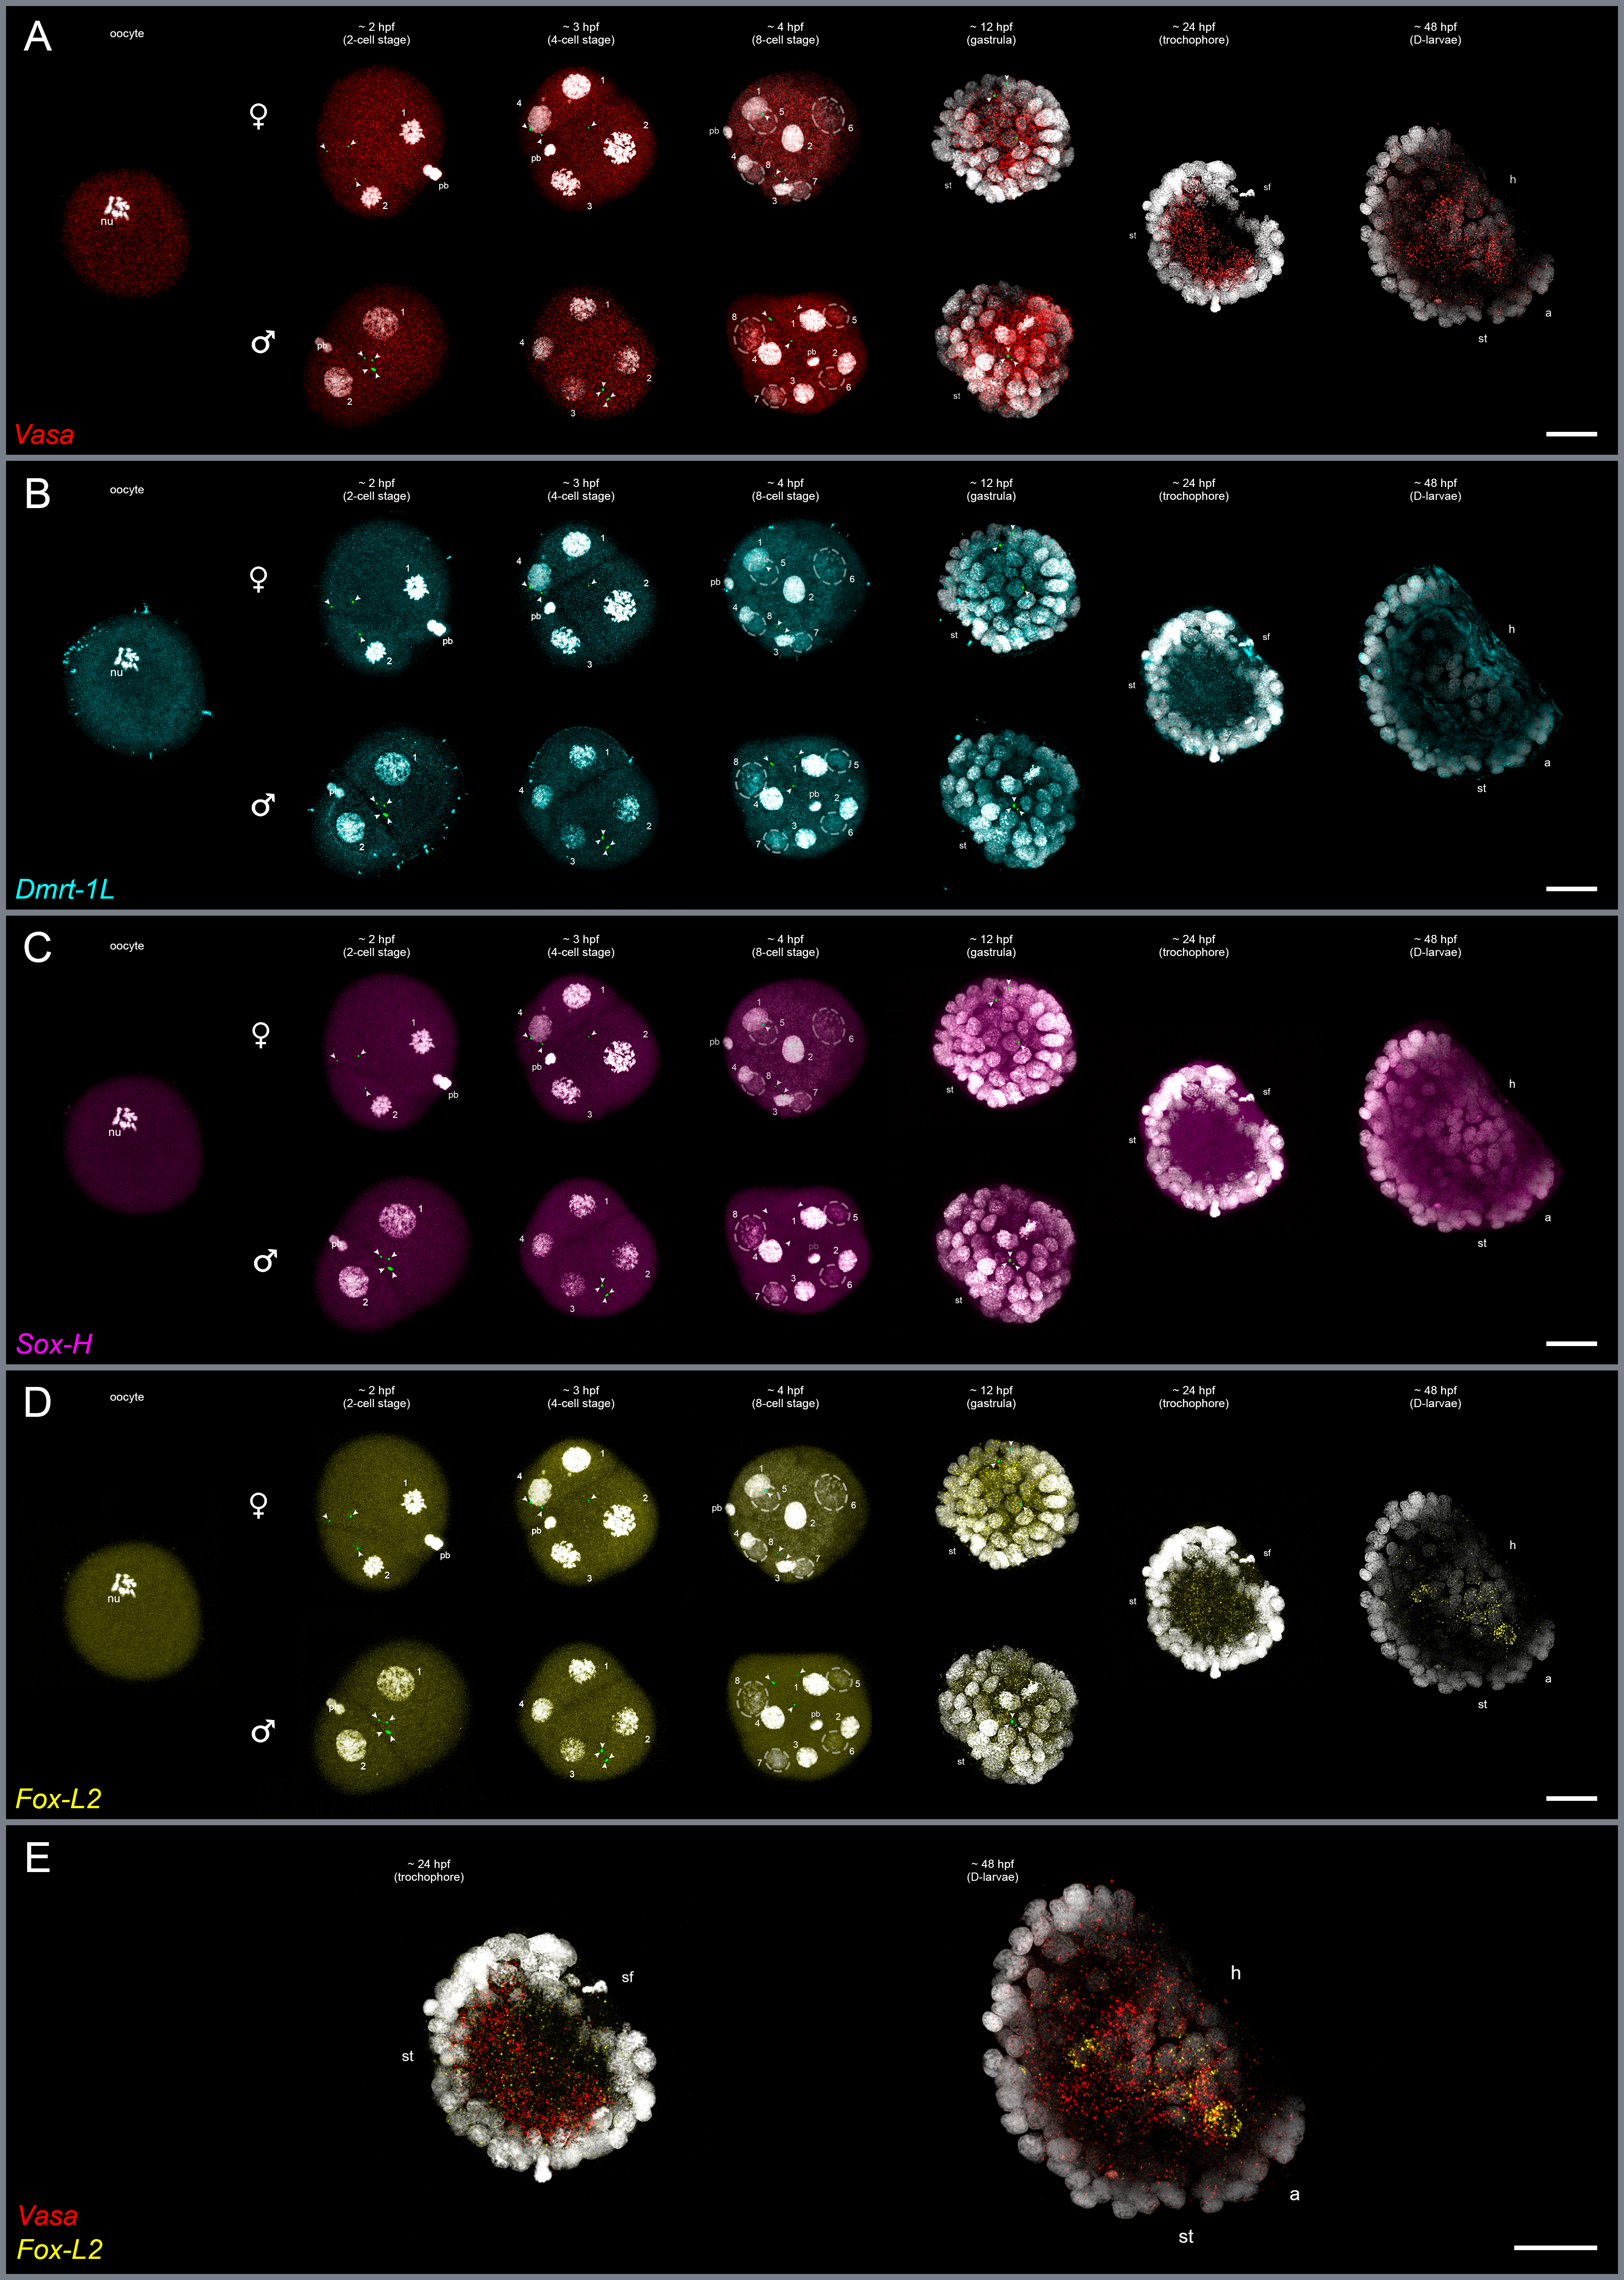
\includegraphics[width=\textwidth]{chapter_molecularEvolution/figure_3.png}
	\caption[\textbf{Distribution of \gls{aasd} of single-copy orthogroups in bivalves (A), including \glspl{dsfg} (B), and their correlations with tip-to-tip distances (C), alignment lengths (D), and number of species (E)}]
	{
		\textbf{Distribution of \gls{aasd} of single-copy orthogroups in bivalves (A), including \glspl{dsfg} (B), and their correlations with tip-to-tip distances (C), alignment lengths (D), and number of species (E)}. The distribution of AASD has been computed on the median values of pairwise distances of $>$11k \glspl{sco} from the reduced bivalve dataset (see main text and \cref{fig:workflow}). Genes have been divided according to their median \gls{aasd} value into three different groups, which are indicated by different colors and increasing numbers (Groups 1, 2, and 3). Circle heights of \glspl{dsfg} show the median value of their \gls{aasd}, while the size indicates the number of represented species. \gls{dsfg} trees are shown on the bottom (full trees can be found in \cref{suppFig:dmrt_bivalves,suppFig:fox_bivalves}). Darker points in C--E indicate \gls{dsfg} \glspl{sco}. The correlation between the amino acid distance and the tip-to-tip distance has been computed on 200 randomly-selected orthogroups.
	}
	\label{fig:DSFG_bivalveDivergence}
\end{figure}

From the distribution of median \gls{aasd}, 112 genes were assigned to Group 1 (\onepercent{} upper quantile), 447 to Group 2 (\fivepercent{} upper quantile), and 10.603 to Group 3. Most of the \glspl{dsfg} (29/32) fell in Group 3 (\cref{fig:DSFG_bivalveDivergence}), which means they have a median \gls{aasd} comparable to the vast majority of other genes in bivalves (median level of the genomes). Just \gls{dmrt-1l}, \textit{Sox-H}, and \textit{Sox-F} showed higher divergences, and have been accordingly placed in Group 2. Overall, pairwise \gls{aasd} proved to be a good approximation of the tip-to-tip distances ($R = 0.84, p < \num{2.2e-16}$, calculated on 200 randomly-selected trees; \cref{fig:DSFG_bivalveDivergence}\textbf{C}), while it showed no influence from the alignment length ($R = 0.11$) or the number of represented species ($R = -0.23$; \cref{fig:DSFG_bivalveDivergence-D,fig:DSFG_bivalveDivergence-E}). Genes from Group 1 and Group 2 are strongly involved in cellular regulatory processes (such as those related to the metabolism of nucleic acids, proteins, and other macromolecules), but also in development and response to external stimuli, as shown by the GO-term enrichment analysis (\cref{tab:enrichedGOs,suppTab:enrichedGOs_complete}).

\begin{landscape}
	\footnotesize
	\begin{longtable}[c]{@{}lll
		S[table-format = 4, exponent-mode = fixed, fixed-exponent = 0] % disable scientific notation
		S[table-format = 3, exponent-mode = fixed, fixed-exponent = 0] % disable scientific notation
		S[table-format = 1.4, exponent-mode = fixed, fixed-exponent = 0, round-mode = places, round-precision = 4]
		@{}}
		\caption[\textbf{Top enriched GO terms for highly-divergent genes of bivalves, mammals, and \textit{Drosophila}}]
		{
			\textbf{Top enriched GO terms for highly-divergent genes of bivalves, mammals, and \textit{Drosophila}}. The extended version of the table, which includes also the expected number of annotated genes per GO term and all the other enriched GO terms, can be accessed in \cref{suppTab:enrichedGOs_complete}.
		}
		\label{tab:enrichedGOs}                                                                                                                                                                                                                                                                                                                                                                                \\
		\toprule
		\multicolumn{1}{c}{\textbf{Dataset}}           & \multicolumn{1}{c}{\textbf{GO.ID}} & \multicolumn{1}{c}{\textbf{Term}}                                         & \textbf{\begin{tabular}[c]{@{}c@{}}Annotated\\ genes\end{tabular}} & \textbf{\begin{tabular}[c]{@{}c@{}}Significant\\ genes\end{tabular}} & \multicolumn{1}{c}{\textbf{\begin{tabular}[c]{@{}c@{}}Classic\\ Fisher\end{tabular}}} \\* \midrule \midrule
		\endfirsthead
		%
		\multicolumn{6}{c}%
		{\textbf{Tab. \thetable} continued from previous page}                                                                                                                                                                                                                                                                                                                                             \\
		\toprule
		\multicolumn{1}{c}{\textbf{Dataset}}           & \multicolumn{1}{c}{\textbf{GO.ID}} & \multicolumn{1}{c}{\textbf{Term}}                                         & \textbf{\begin{tabular}[c]{@{}c@{}}Annotated\\ genes\end{tabular}} & \textbf{\begin{tabular}[c]{@{}c@{}}Significant\\ genes\end{tabular}} & \multicolumn{1}{c}{\textbf{\begin{tabular}[c]{@{}c@{}}Classic\\ Fisher\end{tabular}}} \\* \midrule \midrule
		\endhead
		%
		\endfoot
		%
		\endlastfoot
		%
		\multirow{21}{*}{\textbf{Bivalvia}}            & GO:0060255                         & regulation of macromolecule metabolic process                             & 737                                                                & 59                                                                   & 0.04525                                                                                  \\
		                                               & GO:0080090                         & regulation of primary metabolic process                                   & 673                                                                & 53                                                                   & 0.01818                                                                                  \\
		                                               & GO:0019219                         & regulation of nucleobase-containing compound metabolic process            & 541                                                                & 41                                                                   & 0.02388                                                                                  \\
		                                               & GO:0006351                         & DNA-templated transcription                                               & 571                                                                & 39                                                                   & 0.03767                                                                                  \\
		                                               & GO:0032774                         & RNA biosynthetic process                                                  & 579                                                                & 39                                                                   & 0.04490                                                                                  \\
		                                               & GO:0051252                         & regulation of RNA metabolic process                                       & 517                                                                & 37                                                                   & 0.02719                                                                                  \\
		                                               & GO:0006355                         & regulation of DNA-templated transcription                                 & 490                                                                & 35                                                                   & 0.03751                                                                                  \\
		                                               & GO:2001141                         & regulation of RNA biosynthetic process                                    & 491                                                                & 35                                                                   & 0.03844                                                                                  \\
		                                               & GO:0006950                         & response to stress                                                        & 370                                                                & 33                                                                   & 0.01949                                                                                  \\
		                                               & GO:0032502                         & developmental process                                                     & 261                                                                & 27                                                                   & 0.04445                                                                                  \\
		                                               & GO:0006468                         & protein phosphorylation                                                   & 345                                                                & 23                                                                   & 0.02483                                                                                  \\
		                                               & GO:0031325                         & positive regulation of cellular metabolic process                         & 125                                                                & 17                                                                   & 0.00801                                                                                  \\
		                                               & GO:0010604                         & positive regulation of macromolecule metabolic process                    & 151                                                                & 17                                                                   & 0.04047                                                                                  \\
		                                               & GO:0051172                         & negative regulation of nitrogen compound metabolic process                & 117                                                                & 16                                                                   & 0.00814                                                                                  \\
		                                               & GO:0051173                         & positive regulation of nitrogen compound metabolic process                & 137                                                                & 15                                                                   & 0.02454                                                                                  \\
		                                               & GO:0006310                         & DNA recombination                                                         & 66                                                                 & 14                                                                   & 0.00087                                                                                  \\
		                                               & GO:0048513                         & animal organ development                                                  & 83                                                                 & 12                                                                   & 0.04088                                                                                  \\
		                                               & GO:0010629                         & negative regulation of gene expression                                    & 78                                                                 & 11                                                                   & 0.00048                                                                                  \\
		                                               & GO:0023051                         & regulation of signaling                                                   & 133                                                                & 11                                                                   & 0.02872                                                                                  \\
		                                               & GO:0045934                         & negative regulation of nucleobase-containing compound metabolic process   & 64                                                                 & 11                                                                   & 0.03637                                                                                  \\
		                                               & GO:0009605                         & response to external stimulus                                             & 90                                                                 & 11                                                                   & 0.04544                                                                                  \\
		\multirow{1}{*}{\textbf{Bivalvia}}             & GO:0044419                         & biological process involved in interspecies interaction between organisms & 63                                                                 & 11                                                                   & 0.04761                                                                                  \\* \midrule
		\multirow{22}{*}{\textbf{Mammalia}}            & GO:0006955                         & immune response                                                           & 1297                                                               & 145                                                                  & 0.00061                                                                                  \\
		                                               & GO:0098542                         & defense response to other organism                                        & 853                                                                & 112                                                                  & 0.02066                                                                                  \\
		                                               & GO:0045087                         & innate immune response                                                    & 647                                                                & 82                                                                   & 8.5e-10                                                                                  \\
		                                               & GO:0001817                         & regulation of cytokine production                                         & 630                                                                & 51                                                                   & 0.04660                                                                                  \\
		                                               & GO:0042742                         & defense response to bacterium                                             & 233                                                                & 45                                                                   & 1.7e-07                                                                                  \\
		                                               & GO:0006954                         & inflammatory response                                                     & 642                                                                & 45                                                                   & 0.01735                                                                                  \\
		                                               & GO:0019221                         & cytokine-mediated signaling pathway                                       & 382                                                                & 44                                                                   & 3.9e-07                                                                                  \\
		                                               & GO:0002250                         & adaptive immune response                                                  & 342                                                                & 44                                                                   & 1.3e-05                                                                                  \\
		                                               & GO:0001819                         & positive regulation of cytokine production                                & 402                                                                & 41                                                                   & 0.02723                                                                                  \\
		                                               & GO:0002697                         & regulation of immune effector process                                     & 308                                                                & 37                                                                   & 0.04426                                                                                  \\
		                                               & GO:0042110                         & T cell activation                                                         & 432                                                                & 35                                                                   & 0.02564                                                                                  \\
		                                               & GO:0051607                         & defense response to virus                                                 & 257                                                                & 34                                                                   & 1.9e-07                                                                                  \\
		                                               & GO:0048232                         & male gamete generation                                                    & 491                                                                & 32                                                                   & 0.02255                                                                                  \\
		                                               & GO:0007283                         & spermatogenesis                                                           & 478                                                                & 31                                                                   & 0.02801                                                                                  \\
		                                               & GO:0070661                         & leukocyte proliferation                                                   & 273                                                                & 29                                                                   & 0.01285                                                                                  \\
		                                               & GO:0002449                         & lymphocyte mediated immunity                                              & 221                                                                & 29                                                                   & 0.04833                                                                                  \\
		                                               & GO:0070663                         & regulation of leukocyte proliferation                                     & 212                                                                & 25                                                                   & 0.01870                                                                                  \\
		                                               & GO:0050727                         & regulation of inflammatory response                                       & 300                                                                & 24                                                                   & 0.00235                                                                                  \\
		                                               & GO:0031349                         & positive regulation of defense response                                   & 240                                                                & 24                                                                   & 0.01239                                                                                  \\
		                                               & GO:0002768                         & immune response-regulating cell surface receptor signaling pathway        & 177                                                                & 22                                                                   & 0.00336                                                                                  \\
		                                               & GO:0050829                         & defense response to Gram-negative bacterium                               & 66                                                                 & 17                                                                   & 1.7e-10                                                                                  \\
		                                               & GO:0071222                         & cellular response to lipopolysaccharide                                   & 164                                                                & 17                                                                   & 0.00012                                                                                  \\
		\multirow{13}{*}{\textbf{Mammalia}}            & GO:0010466                         & negative regulation of peptidase activity                                 & 163                                                                & 16                                                                   & 0.00036                                                                                  \\
		                                               & GO:0002429                         & immune response-activating cell surface receptor signaling pathway        & 164                                                                & 16                                                                   & 0.00243                                                                                  \\
		                                               & GO:1903555                         & regulation of tumor necrosis factor superfamily cytokine production       & 137                                                                & 16                                                                   & 0.01244                                                                                  \\
		                                               & GO:0071706                         & tumor necrosis factor superfamily cytokine production                     & 137                                                                & 16                                                                   & 0.01244                                                                                  \\
		                                               & GO:0070665                         & positive regulation of leukocyte proliferation                            & 132                                                                & 16                                                                   & 0.02765                                                                                  \\
		                                               & GO:0045089                         & positive regulation of innate immune response                             & 113                                                                & 16                                                                   & 0.03224                                                                                  \\
		                                               & GO:0071356                         & cellular response to tumor necrosis factor                                & 175                                                                & 15                                                                   & 0.00219                                                                                  \\
		                                               & GO:0002695                         & negative regulation of leukocyte activation                               & 148                                                                & 15                                                                   & 0.01151                                                                                  \\
		                                               & GO:0002456                         & T cell mediated immunity                                                  & 82                                                                 & 15                                                                   & 0.01605                                                                                  \\
		                                               & GO:0002705                         & positive regulation of leukocyte mediated immunity                        & 113                                                                & 15                                                                   & 0.01837                                                                                  \\
		                                               & GO:0032680                         & regulation of tumor necrosis factor production                            & 133                                                                & 15                                                                   & 0.03262                                                                                  \\
		                                               & GO:0032640                         & tumor necrosis factor production                                          & 133                                                                & 15                                                                   & 0.03262                                                                                  \\
		                                               & GO:0050866                         & negative regulation of cell activation                                    & 165                                                                & 15                                                                   & 0.04048                                                                                  \\* \midrule
		\multirow{10}{*}{\textit{\textbf{Drosophila}}} & GO:0000819                         & sister chromatid segregation                                              & 140                                                                & 11                                                                   & 0.02927                                                                                  \\
		                                               & GO:0070192                         & chromosome organization involved in meiotic cell cycle                    & 54                                                                 & 9                                                                    & 0.00849                                                                                  \\
		                                               & GO:0007131                         & reciprocal meiotic recombination                                          & 37                                                                 & 7                                                                    & 0.00066                                                                                  \\
		                                               & GO:0007143                         & female meiotic nuclear division                                           & 54                                                                 & 6                                                                    & 0.02270                                                                                  \\
		                                               & GO:0035967                         & cellular response to topologically incorrect protein                      & 44                                                                 & 5                                                                    & 0.03334                                                                                  \\
		                                               & GO:0035966                         & response to topologically incorrect protein                               & 47                                                                 & 5                                                                    & 0.04266                                                                                  \\
		                                               & GO:0007141                         & male meiosis I                                                            & 13                                                                 & 4                                                                    & 0.00150                                                                                  \\
		                                               & GO:0140543                         & positive regulation of piRNA transcription                                & 3                                                                  & 3                                                                    & 6.9e-05                                                                                  \\
		                                               & GO:0010526                         & retrotransposon silencing                                                 & 8                                                                  & 3                                                                    & 0.00331                                                                                  \\
		                                               & GO:0007130                         & synaptonemal complex assembly                                             & 10                                                                 & 3                                                                    & 0.00666                                                                                  \\
		\multirow{5}{*}{\textit{\textbf{Drosophila}}}  & GO:0030719                         & P granule organization                                                    & 11                                                                 & 3                                                                    & 0.00888                                                                                  \\
		                                               & GO:0071218                         & cellular response to misfolded protein                                    & 12                                                                 & 3                                                                    & 0.01149                                                                                  \\
		                                               & GO:0051788                         & response to misfolded protein                                             & 12                                                                 & 3                                                                    & 0.01149                                                                                  \\
		                                               & GO:0007135                         & meiosis II                                                                & 15                                                                 & 3                                                                    & 0.02169                                                                                  \\
		                                               & GO:0034508                         & centromere complex assembly                                               & 19                                                                 & 3                                                                    & 0.04094                                                                                  \\* \bottomrule \bottomrule
	\end{longtable}
\end{landscape}

\subsection{Dmrt, Sox, and Fox genes, and amino acid sequence divergence in the test datasets} \label{subSect:dsfgTestDataset}
The \gls{dsfg} datasets retrieved in mammals and fruit flies are far more complete than those in bivalves, and most of the already-recognised orthology groups have been identified.

In mammals, we retrieved 7 \gls{dmrt} orthology groups with about \qty{3.1}{\percent} of missing data, 20 \gls{sox} orthology groups with about \qty{8.1}{\percent} of missing data, and 42 \gls{fox} orthology groups with about \qty{4.6}{\percent} of missing data (\cref{suppFig:DSFG_testCompilation-A,suppFig:dmrt_mammals,suppFig:fox_mammals,suppTab:dsfg_mammalAnnotation}). Of these, just \textit{Sox-5} was not included in the subsequent \gls{aasd} analysis, as it did not meet the \qty{50}{\percent}-species occupancy threshold. OrthoFinder analysed about \qty{650}{\mega\nothing} genes, and the number of \glspl{sco} used in the \gls{aasd} analysis (thus resulting from the DISCO-based orthogroup decomposition pipeline) is \qty{> 16}{\kilo\nothing} (\cref{fig:DSFG_testDivergence-A}). From the distribution of median \gls{aasd}, \num{163} genes were assigned to Group 1, \num{649} to Group 2, and \noexponentnum{15355} to Group 3. Most of the \glspl{dsfg} (66/68) fell in Group 3 (\cref{fig:DSFG_testDivergence-B}), while \gls{sry} and \textit{Fox-D4} showed higher divergences, and have been accordingly placed in Group 1 and Group 2, respectively. Highly-divergent genes show a strong enrichment in immune-related functions (such as innate and adaptive immune response, defence response to bacteria and viruses, lymphocyte methabolism, etc.), but also in reproductive processes (such as spermatogenesis; \cref{tab:enrichedGOs,suppTab:enrichedGOs_complete}).

Concerning \textit{Drosophila}, we retrieved 4 \gls{dmrt} orthology groups with about \qty{1.7}{\percent} of missing data, 7 \gls{sox} orthology groups with about \qty{3.9}{\percent} of missing data, and 17 \gls{fox} genes with about \qty{8.3}{\percent} of missing data (\cref{suppFig:DSFG_testCompilation-B,suppFig:dmrt_drosophila,suppFig:fox_drosophila,suppTab:dsfg_drosophilaAnnotation}). OrthoFinder analysed about \qty{240}{\mega\nothing}, and the distribution of median \gls{aasd} was built after $>$12k \glspl{sco} (\cref{fig:DSFG_testDivergence-C}). \num{126} genes were assigned to Group 1, \num{501} to Group 2, and \noexponentnum{11880} to Group 3. All of the \glspl{dsfg} have been used in the \gls{aasd} analysis, but none of them have been placed in Group 1 or 2, that is, all the \glspl{dsfg} in \textit{Drosophila} have an \gls{aasd} comparable to the median level of the genome (\cref{fig:DSFG_testDivergence-D}). Genes of Group 1 and Group 2 show a GO-term enrichment in meiotic processes, such as chromosome/chromatid organisation, and retrotransposon silencing (\cref{tab:enrichedGOs,suppTab:enrichedGOs_complete}).

\begin{figure}
	\centering
	\includegraphics[width=0.9\textwidth]{chapter_molecularEvolution/figure_4.png}
	\captionsetup[subfigure]{labelformat=nocaption}
	\begin{subfigure}{0\linewidth}
	\caption{}\label{fig:DSFG_testDivergence-A}
	\end{subfigure}% <----- get rid of space, for proper centering
	\begin{subfigure}{0\linewidth}
	\caption{}\label{fig:DSFG_testDivergence-B}
	\end{subfigure}% <----- get rid of space, for proper centering
	\begin{subfigure}{0\linewidth}
	\caption{}\label{fig:DSFG_testDivergence-C}
	\end{subfigure}% <----- get rid of space, for proper centering
	\begin{subfigure}{0\linewidth}
	\caption{}\label{fig:DSFG_testDivergence-D}
	\end{subfigure}
	\caption[\textbf{Distribution of \gls{aasd} of single-copy orthogroups in Mammalia (A) and \textit{Drosophila} (C), including \gls{dsfg} (B-D)}]
	{
		\textbf{Distribution of \gls{aasd} of single-copy orthogroups in Mammalia (A) and \textit{Drosophila} (C), including \gls{dsfg} (B-D)}. The distributions of AASD in mammals and fruit flies have been computed on the median values of pairwise distances of over 16k and 12k SCOs, respectively. Genes have been divided according to their median AASD value into three different groups, which are indicated by different colors and increasing numbers (Groups 1, 2, and 3). Circle heights of DSFGs show the median value of their AASD, while the size indicates the number of represented species. DSFG trees are shown on the bottom (full trees can be found in \cref{suppFig:dmrt_mammals,suppFig:sox_mammals,suppFig:fox_mammals} for mammals and in \cref{suppFig:dmrt_drosophila,suppFig:sox_drosophila,suppFig:fox_drosophila} for fruit flies). Insets: scheme of the sex-determination molecular pathways in \textit{Mus musculus} and in \textit{Drosophila melanogaster}, with shown the main genes involved (adapted from \citebold{beukeboom2014evolution}). Green arrows indicate transcription activations, red arrows indicate transcription suppressions. X: sex chromosomes; A: autosomal chromosomes; \textit{DSX\textsuperscript{M/F}}: \textit{DSX} splicing variants present in males or females, respectively.
	}
	\label{fig:DSFG_testDivergence}
\end{figure}

\section{Discussion} \label{chpater3-discussion}
\subsection{A new manually-curated and phylogenetic-based reference dataset of Dmrt, Sox, and Fox genes in bivalves}
The annotation and characterisation process of a gene family in a certain clade of organisms may harbour many overlooked challenges (\citebold{vizueta2020bitacora}). For example, the presence of highly-conserved catalytic domains may hamper the correct identification of the components of a gene family because of insufficient phylogenetic signal, as it is the case for Hox and ParaHox genes and their homeobox motif (\citebold{baldwin2018new, nicolini2023comparative}). Conversely, the components of dynamic gene families characterised by abrupt and sequential duplication events may be difficult to sort into separate groups. As a matter of fact, varying levels of sequence heterogeneity and gene copy numbers makes the inference of orthologous groups hard, as for certain clans of the P450 gene family (\citebold{dermauw2020diversity}). Regardless of the causes, having a solid and wide phylogenetic context in which to study gene duplications and losses, and orthology relationships, is crucial to overcome these difficulties. In the same way, manual curation and visual inspection of multiple sequence alignments, phylogenetic trees, and gene structures (in terms of domain composition, start and stop codons, and other feature representations) is helpful, despite being time-demanding and possibly low reproducible. In this study, we characterised the full complement of \glspl{dsfg} in the vast class of bivalves, by leveraging sequence domain annotation, phylogenetics, and manual curation of the dataset. Our aim was to obtain the most reliable gene complements as possible, combined with a vast taxonomic dataset, a solid phylogenetic inference, an openly-available dataset of gene sequences, and a reproducible pipeline for the annotation of gene identity. By doing so, we want to provide a reliable resource for future studies of \glspl{dsfg}, either focused on bivalves or generally in Metazoa.

Concerning the \gls{dmrt} gene family, we identified orthologs of the vertebrate \textit{Dmrt-2}, \textit{Dmrt-3}, and \textit{Dmrt-4/5} (or \textit{A1/A2}; \cref{fig:DSFG_bivalveCompilation,suppFig:dmrt_bivalves,suppTab:dsfg_bivalveAnnotation}), which are also expected to have been present in the Bilateria common ancestor (\citebold{mawaribuchi2019independent}). \citeboldyearparent{wang2023genome} found that \textit{Dmrt-4/5} is duplicated in \gls{mmer} and \gls{csin} (Venerida), and in \gls{dpol} (Myida), and we confirm this result by tracing back the duplication event to the split between Palaeoheterdonta (here represented by Unionida) and Heterodonta (here represented by Venerida, Myida, Sphaeriida, Adapedonta, Cardiida, and Lucinida; \cref{fig:DSFG_bivalveCompilation}). Furthermore, we confirm \gls{dmrt-1l} to be present in many bivalve species (mainly belonging to the Ostreida, Pectinida, Mytilida, and Unionida orders; \cref{fig:DSFG_bivalveCompilation}), as well as in gastropods and \textit{Octopus}. Though, our phylogenetic analysis did not retrieve any unambiguous orthology relationship among \gls{dmrt-1l} and either vertebrate \textit{Dmrt-1} or \textit{Drosophila} \gls{dsx} genes, as instead it was proposed in previous works (\citebold{li2018foxl2,evensen2022comparative}). As a matter of fact, the amino acid sequence of the \gls{dmrt-1l} \gls{dm} domain does not recall that of any other \gls{dmrt} gene. Furthermore, it must be considered that various phylogenetic analyses have recovered both \textit{Dmrt-1} and \gls{dsx} genes to be restricted to vertebrates and arthropods, respectively (\citebold{wexler2014pan,mawaribuchi2019independent,panara2019phylogenetic}), that is, they do not have any direct ortholog outside their relative clades. Thus, if \gls{dmrt-1l}, \gls{dsx}, and \textit{Dmrt-1} are true orthologs, their origin would need to be placed at least in the Bilateria common ancestor, which seems however to be not the case. All considered, we thus confirm that \gls{dmrt-1l} is not orthologous to \textit{Dmrt-1} and \gls{dsx} and is rather a mollusc-specific gene (\citebold{evensen2022comparative}). The monophyly of the group is not supported by the phylogenetic tree inferred with \gls{dmrt} genes from molluscs and the reference species (\cref{suppFig:dmrt_bivalves}); though, it is recovered when analysing just genes from mollusc species (\cref{suppFig:dmrt_molluscOnly}). To this regard, we speculate that in our analysis, the difficulty in obtaining the monophyly of \gls{dmrt-1l} genes may have arisen primarily because of the many \gls{cele}-restricted genes (\cref{suppTab:reference_dsfgs}), which are placed among the other bivalve genes (\cref{suppFig:dmrt_bivalves}), but also because of the high \gls{aasd} of \gls{dmrt-1l} genes (see \cref{subsection:molecularEvolution-discussion-highaasd}), which hampers a straight-forward phylogenetic reconstruction. Furthermore, our broad-context analysis allowed us to identify some cases of incorrect gene identification in bivalves, which have arisen because of erroneous or ambiguous annotations in previous works, as a result of limited datasets or analyses. For example, the scallop-specific cluster of \gls{dmrt} genes retrieved by \citeboldyearparent{wang2023genome} rather belongs to the \gls{dmrt-1l} group, while the classification of \gls{dmrt} genes in \textit{Crassostrea} species provided by \citeboldyearparent{zeng2024genome} needs to be revised following the one of this work (\textit{Dmrt-1} genes \textit{sensu}-Zhang are \textit{Dmrt-4/5}; \textit{Dmrt-2} genes \textit{sensu}-Zhang are \textit{Dmrt-3}; \textit{Dmrt-3} genes \textit{sensu}-Zhang are \gls{dmrt-1l}; hence, \textit{Crassostrea} species do not have \textit{Dmrt-2} genes).

For what concerns the \gls{sox} gene family, bivalves (or molluscs) do not show any major clade-restricted gene, as only the five Bilateria-specific \gls{sox} groups (\textit{Sox-B1/2}, \textit{Sox-C}, \textit{Sox-D}, \textit{Sox-E}, and \textit{Sox-F}) and \textit{Sox-H} have been identified (\cref{fig:DSFG_bivalveCompilation,suppFig:sox_bivalves,suppTab:dsfg_bivalveAnnotation}), in accordance with previous findings (\citebold{yu2017genome,evensen2022comparative, wang2024genome}). \textit{Sox-B1/2} is clearly made up of two subgroups (i.e., \textit{Sox-B1} and \textit{Sox-B2}), as expected, but their respective identity could not be unambiguously established, as \textit{Sox-B1/2} genes of reference species do not form separate clusters (\cref{suppFig:sox_bivalves}). Even when inferring the phylogenetic tree only of components of the \textit{Sox-B1/2} group from molluscs and reference species, the identity can not be properly established (\cref{suppFig:sox_B12}).

Compared to \gls{dmrt} and \gls{sox} genes, the \gls{fox} gene family appears as the most dynamic in terms of gene presence/absence, as already shown by other works (\citebold{wu2020identification, seudre2022fox, schomburg2022phylogenetic}). Our phylogenetic analysis successfully recovered Group I and Group II of \gls{fox} genes (\citebold{larroux2008genesis}), which include the four \gls{fox} genes that were present in the Bilateria common ancestor (\textit{Fox-C}, \textit{Fox-F}, \textit{Fox-L1}, and \textit{Fox-Q1}; \cref{fig:DSFG_bivalveCompilation,suppFig:fox_bivalves,suppTab:dsfg_bivalveAnnotation}; \citebold{shimeld2010clustered}). To our knowledge, this is the first broad-taxonomic identification and classification of \gls{fox} genes in bivalves, as up to now they have been systematically characterised only in \gls{cgig} (\citebold{yang2014phylogeny}), \gls{pyes} (now \textit{Mizuhopecten yessoensis}; \citebold{wu2020identification}), and \gls{rphi} (\citebold{liu2024characterization}). Firstly, our analysis confirms the absence in molluscs of \textit{Fox-I}, \textit{Fox-Q1}, \textit{Fox-R}, \textit{Fox-S} (\cref{suppFig:fox_bivalves}), which are in fact thought to have emerged with the diversification of deuterostomes or vertebrates (\citebold{yang2014phylogeny, wu2020identification, seudre2022fox, schomburg2022phylogenetic}). Furthermore, we have found many \gls{fox} groups that appeared as mollusc-specific and/or still-unnamed at a first analysis (\textit{Fox-OG2/NA}, \textit{Fox-OG39/NA}, \textit{Fox-OG15/NA}, and \textit{Fox-OG28-NA}; \cref{suppTab:dsfg_bivalveAnnotation}). However, a more in-depth investigation revealed a different scenario. \textit{Fox-OG2/NA} appears close to the human \textit{Fox-M} gene in the phylogenetic tree, but they do not form a monophyletic group (\cref{suppFig:fox_bivalves}). However, by comparing \textit{Fox-OG2/NA} sequences and phylogenetic tree with those analysed by \citeboldyearparent{yang2014phylogeny}, \citeboldyearparent{wu2020identification}, \citeboldyearparent{schomburg2022phylogenetic}, and \citeboldyearparent{seudre2022fox}, it appears clear that this group of \gls{fox} genes is indeed \textit{Fox-M}. However, our analysis has failed to retrieve a monophyletic relationship among bivalve and human \textit{Fox-M} genes, even when inferring a tree with just \textit{Fox-J2}, \textit{Fox-M}, \textit{Fox-O}, and \textit{Fox-P} complements (\cref{suppFig:fox_JMOP}), which belong to the same \gls{fox} group. Regarding the \textit{Fox-OG39/NA} group, it does not have any homolog in reference species (\cref{suppFig:fox_bivalves}) but is found to belong to the \textit{Fox-AB} group by sequence comparison with previous works (\citebold{yang2014phylogeny, wu2020identification, seudre2022fox}). \textit{Fox-AB} was formerly described only in the sea urchin \gls{spur} and the lancelet \gls{bflo} (\citebold{tu2006sea,yu2008fox}), but was later identified also in several Spiralia lineages, including molluscs (e.g., \citebold{yang2014phylogeny, wu2020identification, seudre2022fox}). A similar situation concerns \textit{Fox-OG15/NA} and \textit{Fox-OG28/NA}, which again could not be named based on orthology relationships with the reference species genes (\cref{suppFig:fox_bivalves}), but actually represent two lineage-specific expansions of the \textit{Fox-Q2} group (named \textit{Fox-Q2b} and \textit{Fox-Q2c}), as already appointed in previous studies (\citebold{yang2014phylogeny, wu2020identification}). This observation fits within the wider context of the \textit{Fox-Q2} group expansion in Bilateria and, particularly, in Spiralia, that led to remarkable differences in their gene copy numbers across various clades (\citebold{seudre2022fox}). Two additional \gls{fox} genes have been previously identified in bivalves, and were named \textit{Sox-Y} and \textit{Sox-Z} (\citebold{yang2014phylogeny, wu2020identification}). In our analysis, these \gls{fox} groups were at first identified as \textit{Fox-OG13/NA} and \textit{Fox-OG16/NA}, after sequence comparison of \gls{fox} genes from \gls{cgig} and \gls{pyes}. On one hand, \textit{Fox-Y} was firstly identified in \gls{spur} (\citebold{tu2006sea}) and only recently in a few bivalve species (\citebold{yang2014phylogeny, wu2020identification}). However, when analysing bivalve and \gls{spur} \gls{fox} genes, we failed in retrieving such a clear orthology relationship, as \gls{spur} \textit{Fox-Y} does not fall within the phylogenetic range of bivalve \textit{Fox-OG13/NA}, which contains the supposed \textit{Fox-Y} orthologs (\cref{suppFig:fox_spur}). Also, the forkhead domains of \textit{Fox-OG13/NA} genes were annotated as \singlecurlyquotes{forkhead domain P} (\cref{suppTab:dsfg_bivalveAnnotation}). On the other hand, \textit{Fox-Z} was firstly identified in bivalves and in several other protostomes, thanks to a phylogenetic work including the brachiopod \gls{lung}, the annelid \gls{ctel}, the scorpion \gls{cscu}, and the centipede \gls{smar} (\citebold{wu2020identification}). However, later works have not recovered this \gls{fox} gene group, even when analysing annelids (\citebold{seudre2022fox}) and panarthropods (\citebold{schomburg2022phylogenetic}) in a more dedicated effort. In this case, the forkhead domains were annotated as either a generic \singlecurlyquotes{forkhead domain} or a \singlecurlyquotes{forkhead domain Q2} (\cref{suppTab:dsfg_bivalveAnnotation}). All considered, we argue that bivalves possess two additional \gls{fox} groups (here \textit{Fox-OG13/NA} and \textit{Fox-OG16/NA}; \cref{fig:DSFG_bivalveCompilation,suppFig:fox_bivalves,suppTab:dsfg_bivalveAnnotation}) which are shared with other mollusc species, as revealed also by other authors. However, given the discordant results of the phylogenetic hypothesis and domain annotation, we think that a more thorough investigation on their orthology relationships with \gls{fox} genes from other Metazoa is needed, and thus we chose to not employ their former names \textit{Fox-Y} and \textit{Fox-Z}.

Besides the \gls{dsfg} groups discussed so far, it must be also considered that many orphan genes have been identified (\cref{suppFig:dmrt_bivalves,suppFig:fox_bivalves,suppTab:dsfg_bivalveAnnotation}). For example, \citeboldyearparent{wu2020identification} identified a duplication event of \textit{Fox-H} genes in \gls{cgig}, which has been recovered also in our analysis for the entire Ostreida clade (\textit{Fox-OG36/NA}; \cref{suppFig:fox_bivalves}). Similarly, a gene orthology group putatively specific to Pteriomorphia has been identified among \gls{sox} genes (\textit{Sox-OG1/NA}). Of course, these genes deserve as much attention as their widely-distributed paralogs, as they may constitute true group-specific expansions and may play fundamental roles in some biological processes. However, they have not been discussed here or included in \cref{fig:DSFG_bivalveCompilation} for clarity purposes, but they are freely available in supplementary materials.

Overall, our analysis clearly shows the importance of adopting a wide-angle approach when characterising the members of a gene family, especially for large ones such as the \gls{fox} genes (\citebold{schomburg2022phylogenetic}). As a matter of fact, the presence of duplication events and orphan genes needs to be addressed with a broad taxonomic dataset, in order to account for possible mis-annotations, gene phylogenetic mis-placements, and sequence heterogeneity. Additionally, many reference species need to be included for the gene identification process, in order to consider distantly-related genes and obtain a solid annotation. Our gene annotation pipeline also resulted to be very solid, even with non-model organisms and sub-optimal genomic and transcriptomic resources, as they are those of bivalves. As a matter of fact, by running the same pipeline on two additional datasets composed of mammal and fruit fly genomes, we were able to obtain high-quality orthology groups in accordance with previous knowledge on the clades (\cref{suppFig:dmrt_mammals,suppFig:fox_drosophila,suppTab:dsfg_mammalAnnotation,suppTab:dsfg_drosophilaAnnotation}), with little or no manual curation needed. Furthermore, this represents also the first broad analysis of \glspl{dsfg} in both mammals and fruit flies, as so far attention has been mainly dedicated to single well-studied organisms or little clades (e.g., \citebold{jackson2010update}).

\subsection{High amino acid sequence divergence identifies putative sex-determining genes} \label{subsection:molecularEvolution-discussion-highaasd}
Sex-biased genes tend to evolve more rapidly than unbiased genes at the level of their protein sequences. Accelerated rates have been observed in both male-biased genes (reviewed in \citebold{parsch2013evolutionary,grath2016sex}) and female-biased genes (e.g., \citebold{papa2017anopheles, ghiselli2018comparative}), but also in \glspl{srg} and primary \glspl{sdg} (\citebold{oNeil1992drosophila_tra, whitfield1993rapid, deBono1996caenorhabditis_tra}). For example, it has been shown that \gls{dmw}, \gls{dmy}, and \gls{sry} (which are \glspl{sdg} in the African clawed frog \gls{xlae}, in the medaka fish \gls{olat}, and in eutherians, respectively) all have higher substitution rates than their paralogues (\textit{Dmrt-1} for \gls{dmw} and \gls{dmy}, \textit{Sox-3} for \gls{sry}), particularly when considering their DNA-binding domains (\citebold{mawaribuchi2012molecular}). Similarly, both a burst of positive selection and a relaxation of purifying selection has been detected in \textit{Drosophila} \gls{sxl} in correspondence with its recruitment at the top of the sex-determing cascade. The same signs of relaxed purifying selection have been found in the downstream targets of \gls{sxl}, that is, \gls{tra} and \gls{dsx}, despite no evidence of positive selection has been detected (\citebold{mullon2012drosophila_sxl}).

Considering these shared features of \glspl{srg} and \glspl{sdg}, we decided to look for signs of accelerated sequence evolution in \glspl{dsfg} of bivalves, in order to evaluate if any of them could be associated with \gls{sd} by employing the tools of molecular evolution. However, we wanted to analyse patterns of sequence evolution not only among putative \glspl{srg} and their close paralogs (as done for \gls{dmrt} genes in \cref{perspective}), but also considering the genomic context in which these genes evolve. In fact, our aim was to check whether higher rates of sequence evolution of \glspl{srg} hold true also when compared to other genes not involved in \gls{sd} and not belonging to the same gene family. To do so, we obtained the \gls{aasd} median values of \qty{> 11}{\kilo\nothing} \glspl{sco} from bivalve genomes (\cref{fig:DSFG_bivalveDivergence-A}), in order to build a statistical distribution to be used as a reference: if \glspl{srg}/\glspl{sdg} (in this case, \glspl{dsfg}) truly evolve faster than other genes, we may expect them to fall within the \fivepercent{} (or even \onepercent{}) upper quantile of the distribution (\cref{fig:DSFG_bivalveDivergence-B}), i.e., within highly divergent genes (Group 1 and Group 2 genes of the distribution; see \cref{chapter:molecularEvolution-MM}). We chose to use the \gls{aasd} as a metric of sequence evolution (instead of the tip-to-tip distances of phylogenetic trees, which account for more comprehensive evolutionary models) in order to save computational time. As a matter of fact, the \gls{aasd} median values proved to be a good approximation of the tip-to-tip median distances in 200 randomly-selected genes (\cref{fig:DSFG_bivalveDivergence-C}; $R = 0.84, p < \num{2.2e-6}$).

Among \glspl{dsfg}, three fell within the \fivepercent{} upper quantile, namely \gls{dmrt-1l}, \textit{Sox-H}, and \textit{Sox-F}. Interestingly, \gls{dmrt-1l} and \textit{Sox-H} have been already proposed to be involved in the male \gls{sd} pathway of \gls{cgig} (\textbf{\textit{inset}} in \cref{fig:DSFG_bivalveDivergence-B}; \citebold{zhang2014genomic}), on the basis of \gls{dge} analyses. Specifically, \textit{Sox-H} (\textit{CgSoxH}) would play a major role in \gls{cgig} \gls{sd}, by interacting with \gls{dmrt-1l} (\textit{CgDsx}) and determining the onset of the male phenotype development; at the same time, both \textit{Sox-H} and \gls{dmrt-1l} would inhibit \textit{Fox-L2} (\textit{CgFoxL2}), which instead is necessary to start the female phenotype development. \gls{dmrt-1l} and \textit{Sox-H} have been appointed several other times to be involved in male-gonad development and differentiation, through \gls{dge} (e.g., \citebold{teaniniuraitemoana2014gonad, capt2018deciphering, afonso2019gonad}), \gls{ish} (e.g., \citebold{naimi2009molecular,li2018foxl2, yue2021variance, liang2019sox2}) and \glsunset{rnai}\glsxtrlong{rnai} (\glsxtrshort{ish}; \citebold{liang2019sox2, sun2022examination}). Therefore, the high \gls{aasd} of \gls{dmrt-1l} and \textit{Sox-H} is coherent with previous works, strengthening their role as putative \glspl{srg}.

The relationship between high gene \gls{aasd} and the involvement in SD is particularly enforced when looking at the patterns of \gls{aasd} in the test datasets, which corroborates the solidity of our analysis:
\begin{inlinelist}
	\item from one side, in the mammal dataset—which represents a strictly genetic \gls{sd} system, thus with a master and rapidly-evolving \gls{sdg}, one of the genes from the \fivepercent{} upper quantile of the distribution is \gls{sry} (\cref{fig:DSFG_testDivergence-A,fig:DSFG_testDivergence-B}), the male sex-determining gene in eutherians (\textbf{\textit{inset}} in \cref{fig:DSFG_testDivergence-B});
	\item from the other side, in the fruit fly dataset—which represents a chromosomic \gls{sd} system, thus without any expected difference in the rates of sequence evolution among \glspl{srg}, none of the \gls{dsfg} exhibit significantly high \gls{aasd} (\cref{fig:DSFG_testDivergence-C,fig:DSFG_testDivergence-D}), including the downstream effector \gls{dsx} (\textit{\textbf{inset}} in \cref{fig:DSFG_testDivergence-D}).
\end{inlinelist}
Also \gls{sxl} and \gls{tra}, both involved in the \gls{sd} pathway of \textit{Drosophila} (\textit{\textbf{inset}} in \cref{fig:DSFG_testDivergence-D}) do not belong to the group of highly-divergent genes, as they have a mean amino acid divergence of about 0.09 and 0.9, respectively (Group 3; \cref{fig:DSFG_testDivergence-D}). Therefore, it can be argued that both \gls{dmrt-1l} and \textit{Sox-H} may not only be \glspl{srg}, but may participate in bivalve \gls{sd} as primary \glspl{sdg}, which is reflected in their high \gls{aasd}, as it is observed for \gls{sry} in mammals. As a matter of fact, if they were involved in \gls{sd} just as intermediate actors of the signalling cascade, then we should have not observed a high \gls{aasd}, as \textit{Drosophila} \gls{sxl}, \gls{tra}, and \gls{dsx} seem to suggest. Overall, these patterns of molecular evolution concerning \glspl{srg} and \gls{sdg} are also supported by the way \gls{sd} regulatory networks evolve. As a matter of fact, it has been proposed that the sex-determining cascades tend to arise and be established with a bottom-up mechanism (\citebold{wilkins1995moving, mullon2012drosophila_sxl, beukeboom2014evolution, capel2017vertebrate}). This means that the regulative relationships among genes at the bottom of the cascade are settled up prior to the regulative relationships among genes at the top and, consequently, upstream regulators are progressively recruited to fine-tune diverse \gls{sd} signals. These evolutionary patterns eventually produce gene-regulatory networks in which the divergence of the upstream triggers is higher than that of downstream effectors, in terms of both identity and sequence composition (\citebold{beukeboom2014evolution}). This mechanism has been proposed for \textit{Drosophila} species (\citebold{mullon2012drosophila_sxl}), \gls{cele} (\citebold{stothard2003sex}), and vertebrates, despite in the latter case has been questioned several times (reviewed in \citebold{capel2017vertebrate}).

At this point, two main objections can be moved against our approach: (1) the distribution of \gls{aasd} is not appropriate for this kind of inference, as it does not represent the true gene evolutionary (or substitution) rates (which instead are those usually employed when dealing with \glspl{srg} and \glspl{sdg}); (2) the three datasets are not comparable one to each other, as they take into consideration very different animal groups, with different taxonomic rankings and different divergence times (thus, the patterns of \gls{aasd} are the products of other confounding factors not directly related to \gls{sd}). Concerning the first objection, we are aware that the \gls{aasd} does not represent the evolutionary rate itself, but rather its product. However, the two features are tightly linked, as on the long term highly-divergent proteins tend to be produced by genes with high evolutionary (or substitution) rates (\citebold{echave2016causes}). By performing a \gls{go}-term enrichment, it emerged that highly-divergent genes of the mammal dataset are mainly involved in the immune response and male spermatogenesis (\cref{tab:enrichedGOs,suppTab:enrichedGOs_complete}), which are two processes notoriously connected with rapid sequence evolution (i.e., higher evolutionary rates; \citebold{swanson2002rapid, murat2023molecular, vinkler2023understanding}). Similarly, highly-divergent genes from the fruit fly dataset show an enrichment for \gls{go}-terms associated with meiotic-related functions (such as the formation of the synaptonemal complex by the products of \textit{c(2)M}, \textit{c(3)G}, \textit{corona}, and \textit{corolla} genes; \cref{tab:enrichedGOs,suppTab:enrichedGOs_complete}), which again are known to be rapidly evolving (\citebold{hemmer2016holding}). In other words, the test datasets---which include well-studied and characterised model systems, allow us to directly link the high \gls{aasd} (as computed in this work) with high rates of sequence evolution (as found in previous works), as they represent well-studied and characterised model systems. This consideration can thus be extended also to the bivalve dataset: highly-divergent genes in terms of \gls{aasd}, which include some \glspl{dsfg} and show an enrichment for \gls{go}-terms associated to macromolecule metabolism and morphological development (\cref{tab:enrichedGOs,suppTab:enrichedGOs_complete}), are also genes with accelerated substitution rates.

Concerning the second objection, we chose two test datasets with different characteristics as we wanted to check the extent of our hypothesis, that is, molecular evolution can be used to look for putative primary \glspl{sdg} in taxonomic-wide analyses. The difference in divergence times and taxonomy ranks for bivalves and therians (Late Cambrian, about \qty{498}{\mya}, \citebold{song2023scaphopoda}; and Early Mesozoic, \qtyrange{166}{123}{\mya}, \citebold{alvarez2022species}, respectively) seems to not influence the sequence diversity of \glspl{srg}, as both \gls{dmrt-1l}/\textit{Sox-H} for bivalves and \gls{sry} for mammals exhibit high \gls{aasd} with respect to their own distributions, regardless of their age. \gls{dmrt-1l} and \textit{Sox-H} (which are mollusc- and Bilateria-specific, respectively) are undoubtedly older than \gls{sry} (which, instead, emerged in the Theria common ancestor; \citebold{foster1992evolution}), but each of them can be considered a highly-divergent gene in bivalves and mammals, respectively (i.e., genes that are included in the \fivepercent{} upper quantile of bivalve and mammal \gls{aasd} distributions). Conversely, the difference in divergence times and taxonomic ranks for \textit{Drosophila} (Paleocene/Eocene boundary, about \qty{56}{\mya}; \citebold{russo2013phylogenetic}) may seem to be influencing the results for the dataset, resulting in a false negative. In other words, it can be argued that:
\begin{inlinelist}
	\item the genes included in the \gls{sd} cascade of \textit{Drosophila} (such as \gls{sxl}, \gls{tra}, and \gls{dsx}; \textbf{\textit{inset}} in \cref{fig:DSFG_testDivergence-D}) have a high \gls{aasd}, which however has not been detected by our methodological approach (for example, this may be traced back to the young diversification age of \textit{Drosophila} species if compared to bivalves);
	\item the species included in the analysis are all congeneric, thus the sequence differentiation of \glspl{srg} may exist not at the amino acid level but at the nucleotide one. 
\end{inlinelist}
To better disentangle this issue and further discuss the fruit fly dataset, we repeated the analysis of the \gls{aasd} only on species of the \textit{Crassostrea} genus (\gls{cgig}, \gls{cang}, \gls{cari}, and \gls{cvir}), which are much younger (Middle Cretaceous, less than \qty{100}{\mya}; \citebold{qi2023construction}), thus comparable to \textit{Drosophila}. Results showed that, even when analysing a smaller bivalve dataset, encompassing only 4 species of recent origin, the high \gls{aasd} of \gls{dmrt-1l} persists, that is, \gls{dmrt-1l} is still grouped together with highly-divergent genes (\cref{suppFig:DSFG_crassostreaDivergence}). The same has not been recovered for \textit{Sox-H}, which fell in genes from Group 3 (the group corresponding to the \qty{95}{\percent} interval of the \gls{aasd} distribution) but still have the second highest \gls{aasd} median value among \glspl{dsfg} (\cref{suppFig:DSFG_crassostreaDivergence}).

Of course we should not expect that highly-divergent genes are only those involved in \gls{sd}, but may participate also in other processes (as discussed earlier and shown by \gls{go}-term enrichments; \cref{tab:enrichedGOs,suppTab:enrichedGOs_complete}). Besides the genes of interest for \gls{sd} (\gls{dmrt-1l}/\textit{Sox-H} for bivalves, and \gls{sry} for mammals), also other components of the \gls{dsfg} families have been retrieved with a high \gls{aasd}, despite they have never been linked directly to \gls{sd} so far: \textit{Sox-F} in bivalves (\cref{fig:DSFG_bivalveDivergence-B}) and \textit{Fox-D4} in mammals (\cref{fig:DSFG_testDivergence-B}). This implies that our approach can\curlyapostrophe t be used to unambiguously identify \glspl{sdg} alone, as high \gls{aasd} is exhibited also by many other genes. Instead, the analysis is meant to be used to detect highly-divergent genes and, subsequently, by comparison with literature and a more thorough and focused functional investigation, putative \glspl{sdg} among them. In this sense, the mammal dataset exemplify the importance of putting the results of our pipeline (as those of any other comparative genomics analysis) into the correct evolutionary and genomic context: among \glspl{dsfg} of mammals, two genes exhibit high \gls{aasd}, one of which is directly related to \gls{sd} (\gls{sry}), while the other has a function connected with neural development (\textit{Fox-D4}; \citebold{klein2013conserved}). Thus, the high \gls{aasd} may arise either because of the involvement in the upper \gls{sd} pathway or because of other life-history traits connected with the gene, respectively. Regarding bivalves, \gls{dmrt-1l} and \textit{Sox-H} show a sharp connection with \gls{sd} as a putative primary \gls{sdg}, either when considering their molecular evolutionary features or when looking at their gene expression and possible function in gonad development (\citebold{naimi2009molecular, teaniniuraitemoana2014gonad, zhang2014genomic, capt2018deciphering, li2018foxl2, afonso2019gonad, liang2019sox2, yue2021variance}). It is difficult to further speculate on the actual involvement in \gls{sd} of \gls{dmrt-1l} and \textit{Sox-H} without any additional information on their biology. Nonetheless, molecular evolution proves to be a valuable tool to investigate genes putatively involved in \gls{sd}, and to identify major targets onto which dedicate future research effort.

\section{Conclusions} \label{chapter:molecularEvolution-conclusions}
Genes functioning in reproductive processes, and particularly \gls{sd}, are often among the most variable in animal genomes, in terms of both sequence composition and regulatory interactions (\citebold{swanson2002rapid,bachtrog2014sex}). Such high evolutionary rates may be traced back both to adaptive evolution (either as natural or sexual selection) or to non-adaptive processes (\citebold{vicoso2006evolutionXchrom,meisel2013faster,parsch2013evolutionary,grath2016sex}), and often results in striking differences in reproductive and sexual systems even among closely-related species. In the present work we took advantage of this characteristic to identify \glspl{sdg} in bivalves among the \gls{dsfg} families. By comprehensively analysing the phylogenetic history and \gls{aasd} in a broad taxonomic dataset, we appointed \gls{dmrt-1l} and \textit{Sox-H} as putative \glspl{sdg}, thus confirming results in previous works that found them to be transcribed in a male-biased manner and/or strongly involved in male-gonad formation (\citebold{naimi2009molecular,teaniniuraitemoana2014gonad,zhang2014genomic,capt2018deciphering,li2018foxl2,afonso2019gonad,liang2019sox2,yue2021variance}). Future studies would now need to further investigate their evolutionary history. For example, considering that \glspl{srg} tend to accumulate in the genomic neighbourhood where primary \glspl{sdg} are located (\citebold{capel2017vertebrate}), analysing the genomic location of \glspl{dsfg} in bivalve genomes may provide enlightening results. Similarly, revealing the genetic interactions of \gls{dmrt-1l} and \textit{Sox-H}, through functional and genome editing assays, would undoubtedly benefit our understanding of their role in the sexual processes of bivalves.

% \end{document}
% \documentclass[../main.tex]{subfiles}

% \begin{document}

{
\setstretch{1.0}
\chapter[Localisation of sex-determination genes and Vasa/\textnormal{Vasa}]{Localisation of three sex-related genes and the germline marker \textit{Vasa}/Vasa in the early developmental stages of \textit{Mytilus galloprovincialis}}
\label{chapter:insitu}
}

{
\setstretch{1.5}
\noindent{\large{Filippo Nicolini\textsuperscript{1,2}, Sergey Nuzhdin\textsuperscript{3}, Fabrizio Ghiselli\textsuperscript{1}, Andrea Luchetti\textsuperscript{1}, Liliana Milani\textsuperscript{1}}}
}

\vspace{5mm}

{
\setstretch{1.0}
\noindent{\textsuperscript{1}\textit{Department of Biological, Geological and Environmental Science, University of Bologna, Bologna (BO), Italy}.}

\noindent{\textsuperscript{2}\textit{Fano Marine Center, Fano (PU), Italy}.}

\noindent{\textsuperscript{3}\textit{3Department of Molecular and Computational Biology, University of Southern California, Los Angeles, CA, USA}.}

\vspace{5mm}

\noindent{\textbf{\textit{Manuscript in preparation.}}}
}

\newpage

\section{Introduction} \label{chapter:insitu-introduction}

Despite the huge socio-economic and scientific importance of bivalves, the knowledge concerning the genetic and molecular bases of their \gls{sd} system is scarce and overlooked (\citebold{breton2018sex, nicolini2023bivalves}). Several components of the \gls{dsfg} families have been appointed as directly involved in \gls{sd} by many works, mainly thanks to \gls{dge} analyses (e.g., \citebold{milani2013nuclear, zhang2014genomic, capt2018deciphering, shi2018proteome}), mRNA/protein visualisation (\citebold{li2018draft,liang2019sox2,wang2020identification,sun2022examination}), \gls{rnai} (\citebold{liang2019sox2,wang2020identification,sun2022examination}) and \gls{qrt-pcr} (\citebold{li2018draft,liang2019sox2,wang2020identification,sun2022examination}). For example, \citeboldyearparent{li2018foxl2} found that \textit{Fox-L2} and \gls{dmrt-1l} are predominantly transcribed in ovaries and testes, respectively, of the Yesso scallop \gls{pyes}, and that they contribute to establish the sexual identity of immature follicles at the molecular level prior to the morphological level. \citeboldyearparent{liang2019sox2} showed that \textit{Sox-2} is involved in the differentiation of male gonads and spermatogenesis of the scallop \gls{cfar}, and that the knocked-out phenotype results in severe loss of both germ-cell mass and spermatogonia. \citeboldyearparent{wang2020identification} speculated that \textit{Fox-L2} is involved in the sex differentiation of female gonads in the freshwater mussel \gls{hcum}. Overall, considerable effort has been made to characterise the transcription patterns of \glspl{dsfg} of interest during the adult stage of bivalves, covering various reproductive phases, while little attention has been given to the embryo and larval stages. Nonetheless, early animal development may represent a crucial moment to the establishment of the sexual identity, as the transcription of \glspl{srg} and \gls{sd} itself begins much earlier than the onset of gonad development and differentiation (even as early as the zygote formation; \citebold{richardson2023comparativeSex}). In mammals, for example, the transcription of \glspl{srg} can be detected during the embryo preimplantation stage (before \qty{4.5}{\dpf}; reviewed in \citebold{richardson2023comparativeSex}), while \gls{sry} realises its function as the male \gls{sdg} at 10.5 days post coitum (\citebold{beukeboom2014evolution}). In \gls{dmel}, the early female splicing variant of \gls{sxl}---which is the top regulator of the \gls{sd} cascade and is activated by a mechanism of chromosome counting (\textbf{\textit{inset}} in \cref{fig:DSFG_testDivergence-D}), is transcribed during the syncytial stages of the embryo (i.e., before \qty{2}{\hpf}; \citebold{salz2010sex}), when it establishes the sexual identity of the embryo through a cell-autonomous mechanism. Therefore, the study of bivalve \gls{sd} necessarily requires to consider also the early stages of embryonic and larval development, in order to obtain a comprehensive scenario of the process. Among bivalves, several species may constitute a model system particularly suitable to study the \gls{sd} process during embryogenesis, because of the presence of the \gls{dui} of mitochondria. This process---which involves the uniparental transmission of the maternal and paternal mitochondrial genomes through eggs and sperm, respectively, allows for an \textit{a-priori} detection of the sexual identity of developing embryos, as early as the first cleavage division of the zygote: in female embryos, the sperm-inherited mitochondria assume a dispersed pattern between blastomeres; conversely, in males the sperm-inherited mitochondria stay assembled together, remain within one blastomere, and are eventually included in \glspl{pgc} (\citebold{zouros2013biparental,ghiselli2019natural}).

Here we sought to expand the knowledge on the process of bivalve \gls{sd}, by employing the Mediterranean mussel \gls{mgal} as a study system, which is a species exhibiting \gls{dui}. Particularly, we aimed to investigate the transcription patterns of three \gls{dsfg} (namely, \pac{dmrt-1l}, \textit{Sox-H}, and \textit{Fox-L2}) during embryo and early larval stages. To this purpose, (i) we first performed a time-series \gls{dge} analysis by using the RNA-sequencing data published by \citeboldyearparent{miglioli2024hcrMytilus}; afterwards, (ii) we investigated the temporal and spatial transcription patterns of the \glspl{dsfg} of interest through mRNA \textit{in-situ} \gls{hcr}. To obtain a more comprehensive developmental context for the transcription patterns of \glspl{dsfg}, (iii) we also traced for the first time in \gls{mgal} the process of the germline specification through mRNA \textit{in-situ} \gls{hcr} and immunolocalization of \textit{Vasa}/Vasa, which is a traditionally-recognised marker of \glspl{pgc} and \glspl{gc} across Metazoa (\citebold{extavour2003mechanisms}). The specification and differentiation of \glspl{gc} (which are part of the gonadal tissue in adults) is in fact a critical process in sexually reproducing multicellular organisms, as it provides the groundwork for the subsequent differentiation of sexually dimorphic gametes. Therefore, understanding the developmental pathway leading to the establishment of \glspl{pgc} and \glspl{gc} is essential to fully characterise the sex-determining process and how the sexual fate of \glspl{pgc}/\glspl{gc} is directed.

\section{Materials and methods} \label{chapter:insitu-MM}
\subsection{Time-series gene expression}
\citeboldyearparent{miglioli2024hcrMytilus} recently produced one of the very first detailed developmental transcriptomes of the Mediterranean mussel \gls{mgal}, spanning from the unfertilized oocyte to the larval stage at \qty{72}{\hpf}, with time points sampled every \qty{4}{\hpf}. A total of thirty different mRNA libraries was sequenced, consisting of fifteen developmental time points per two biological replicates each (\cref{suppTab:readMappings}). These data are extremely useful to thoroughly investigate the transcription patterns of genes throughout the first three days of the \gls{mgal} development, to quantify the transcription level of target genes to be investigated with mRNA \gls{hcr} experiments and to have an overview of the possible outcome from such analysis.

Raw reads were downloaded from the Sequence Read Archive (SRA) in NCBI (BioProject: PRJNA996031) and trimmed using Trimmomatic v0.39 (\citebold{bolger2014trimmomatic}; \verb|LEADING:5| \verb|TRAILING:5 SLIDINGWINDOW:4:15 MINLEN:65|). Read quality was checked using FastQC v0.12.1 (\citebold{andrews2010fastqc}). Trimmed reads were mapped against the \gls{mgal} annotated genome (GCA\_900618805.1; \citebold{gerdol2020massive}) using STAR v2.7.10b (\citebold{dobin2013star}) in \singlecurlyquotes{alignReads} mode with default parameters. The resulting gene count matrix was extracted with StringTie v2.2.1 (\citebold{pertea2015stringtie,pertea2016stringtie}) in expression estimation mode followed by the python script \singlecurlyquotes{prepDE.py} (\verb|-l 99|).

The resulting matrix was processed in R. Raw gene counts were normalised using the median of ratios method as implemented by the DESeq2 package (\citebold{love2014deseq2}), and then transformed through the DESeq2 variance stabilising transformation (vst). Transformed gene counts were used to run a \gls{pca} and visualise sample clustering, and to plot expression values of \textit{Vasa}, \gls{dmrt-1l}, \textit{Sox-H}, and \textit{Fox-L2} (hereafter collectively referred to as \singlecurlyquotes{target genes}). Normalised gene counts were instead used to run a time-series \gls{dge} analysis in \singlecurlyquotes{maSigPro} (\citebold{conesa2006masigpro}).

The entire pipeline was automated through custom python and bash scripts, which are available in a private repository on GitHub.

\subsection{Sample collection, MitoTracker staining and fixation}
Adult mussels were hand collected from various locations surrounding the AltaSea institute at the port of Los Angeles (CA, USA). Sampling took place during the spawning season of the species in California, i.e., from October 2023 to early January 2024.

Selected mussels were thoroughly cleaned from epibionts and placed in ice for approximately 30--60 minutes, then transferred in \gls{fasw} at \qty{16}{\degreeCelsius} and acclimatised for 30 minutes. All the individuals were then placed in a common tank and spawning was induced by cyclical thermal shock, that is, by exposing mussels alternatively to \gls{fasw} at \qtyrange{24}{26}{\degreeCelsius} and \qtyrange{14}{16}{\degreeCelsius} for a time of \qtyrange{30}{40}{\minute} each. As soon as mussels started spawning, individuals were promptly removed from the common tank, carefully washed, air dried to remove contaminant gametes from the shell, and then allowed to continue spawning in isolated containers of about \qty{250}{\ml} with \qty{16}{\degreeCelsius} \gls{fasw}.

Both single and multiple crosses were performed: two males (M1, M2) and two females (F1, F2) were employed for single crosses; six males and six females were employed for multiple crosses, and gametes from the same sex were mixed. One hour after the spawning started, oocytes were filtered through a \num{75} over a \qty{30}{\um} mesh, and aged in \qty{1}{\l} of \gls{fasw} for \qtyrange{40}{60}{\minute}, to allow them to assume a proper circular shape. Oocyte abundance was estimated under a stereomicroscope by eye counting the number of gametes in five aliquots of \qty{1}{\ml}, and then calculating the mean value. Sperm mitochondria were labelled with MitoTracker Red CMXRos (Thermo Fisher Scientific) at a working concentration of \qty{500}{\nano\molar} for \qty{30}{\minute}. MitoTracker is a fluorescent, vital and fixation-resistant mitochondrial dye and was used to be able to detect the sex of developing embryos (as early as the two-blastomere stage) according to the distribution pattern of sperm mitochondria (\citebold{cao2004differential,obata2005specific}). From this step onward, samples were always kept in the dark.

Fertilisation was performed by mixing oocytes and sperm at a ratio of 1:10. Fertilisation success was checked after \qtyrange{20}{30}{\minute} by the formation of polar bodies. The suspension was then carefully washed on a \qty{30}{\um} mesh to remove excess sperm, and brought to a concentration of \qty{250}{\zygotes\per\ml}. The resulting suspension was transferred into cell-culture flasks of \qty{40}{\ml} and embryos/larvae were reared at \qty{16(1)}{\degreeCelsius} in the dark. Water was changed every \qty{24}{\hour}. After \qty{48}{\hpf}, larvae were fed with the unicellular microalgae \textit{Isochrysis galbana}, at a final concentration of about \qty{100000}{\cells\per\ml} following \citeboldyearparent{helm2004hatchery}.

Embryos/larvae were sampled at \qtylist{1;2;3;4}{\hpf}, and then every \qty{12}{\hour} until \qty{72}{\hpf}. Proper development and vitality were checked under a stereomicroscope at every sampling time. After concentration with a mesh of proper size, embryos/larvae were fixed in \qty{3.2}{\percent} \gls{pfa} in \gls{pbs} at \qty{4}{\degreeCelsius} overnight under constant and gentle shaking. \gls{pbs} was prepared with the following concentrations: \qty{128}{\milli\molar} \ce{NaCl}, \qty{2}{\milli\molar} \ce{KCl}, \qty{8}{\milli\molar} \ce{Na2HPO4*2H2O}, and \qty{2}{\milli\molar} \ce{KH2PO4}. Fixed samples were washed 3×\qty{20}{min} in \gls{pbstw} and then dehydrated 3×\qty{30}{\minute} in absolute methanol at \gls{rt}. Dehydrated samples were stored at \qty{-20}{\degreeCelsius} until usage.

\subsection{mRNA \textit{in-situ} hybridization chain reaction (HCR)}
\subsubsection{HCR probe design}
\textit{Vasa}, \gls{dmrt-1l}, \textit{Sox-H}, and \textit{Fox-L2} (the latter three are hereafter referred to as \pac{srg}) spliced-transcript nucleotide sequences of \gls{mgal} were obtained from the previous analyses with OrthoFinder v2.5.5 (\citebold{emms2019orthofinder}) on annotated bivalve genomes and transcriptomes (see \cref{chapter:molecularEvolution-MM}). Accession numbers of spliced transcripts are 10B017427, 10B093608, 10B014180, and 10B094018, respectively. The \singlecurlyquotes{insitu\_probe\_generator} script from the Ozpolat Lab (\citebold{kuehn2022probegenerator}) was used to generate pairs of probes specifically designed for third-generation \gls{hcr} (\citebold{choi2018hcr3}). The built-in BLASTN search against the annotated \gls{mgal} transcriptome was employed to check for putative off-target bindings of probe pairs. B1-488, B2-647, B3-546, and B4-700 pairs of \gls{hcr} amplifiers and fluorophores were chosen, as reported in \cref{tab:fluorescent_dyes}. Resulting probes were synthesised by Integrated DNA Techonologies (IDT\texttrademark) in separate oligo pools.

\afterpage{
\footnotesize
\begin{longtable}[c]{llcccc}
    \caption[\textbf{Characteristics of fluorescent dyes used for each labelled target}]
    {
        \textbf{Characteristics of fluorescent dyes used for each labelled target}. \gls{hcr} amplifiers and the number of probe sets (as in \cref{suppTab:HCRprobes}) are reported when applicable. Dyes for both \textit{Vasa} and Vasa are reported.
    }
    \label{tab:fluorescent_dyes}\\
    %
    \toprule
    \textbf{Target}                                              & \textbf{Dye}                                                     & \textbf{\begin{tabular}[c]{@{}c@{}}HCR\\ amplifier\end{tabular}} & \multicolumn{1}{c}{\textbf{\begin{tabular}[c]{@{}c@{}}HCR\\ probe pairs\end{tabular}}} & \multicolumn{1}{c}{\textbf{\begin{tabular}[c]{@{}c@{}}Excitation\\ (nm)\end{tabular}}} & \multicolumn{1}{c}{\textbf{\begin{tabular}[c]{@{}c@{}}Emission\\ (nm)\end{tabular}}} \\* \midrule \midrule
    \endfirsthead
    \toprule
    \textbf{Target}                                              & \textbf{Dye}                                                     & \textbf{\begin{tabular}[c]{@{}c@{}}HCR\\ amplifier\end{tabular}} & \multicolumn{1}{c}{\textbf{\begin{tabular}[c]{@{}c@{}}HCR\\ probe pairs\end{tabular}}} & \multicolumn{1}{c}{\textbf{\begin{tabular}[c]{@{}c@{}}Excitation\\ (nm)\end{tabular}}} & \multicolumn{1}{c}{\textbf{\begin{tabular}[c]{@{}c@{}}Emission\\ (nm)\end{tabular}}} \\* \midrule \midrule
    \endhead
    %
    \begin{tabular}[c]{@{}l@{}}dsDNA\\ (nuclei)\end{tabular}                                               & DAPI                                                             & \NA                                                              & \NA                                                                                    & 360                                                                                    & 460                                                                                  \\ [0.6cm]
    \begin{tabular}[c]{@{}l@{}}Sperm\\ mitochondria\end{tabular}                                           & \begin{tabular}[c]{@{}l@{}}MitoTracker\\ Red CMXRos\end{tabular} & \NA                                                              & \NA                                                                                    & 575                                                                                    & 600                                                                                  \\ [0.6cm]
    \textit{Vasa}/Vasa & ALEXA-488/-488    & B1/\NA                  & 33/\NA                                        & 499                                                                                    & 520                                                                                  \\* [0.3cm]
    \textit{Dmrt-1L}                                             & ALEXA-647                                                        & B2                                                               & 18                                                                                     & 653                                                                                    & 670                                                                                  \\ [0.3cm]
    \textit{Sox-H}                                               & ALEXA-546                                                        & B3                                                               & 22                                                                                     & 557                                                                                    & 575                                                                                  \\ [0.3cm]
    \textit{Fox-L2}                                              & ALEXA-700                                                        & B4                                                               & 28                                                                                     & 685                                                                                    & 700                                                                                 \\* \bottomrule \bottomrule
\end{longtable}
}

\subsubsection{mRNA \textit{in-situ} HCR and microscope imaging}
mRNA \textit{in-situ} \gls{hcr} in \gls{mgal} embryos was performed following \citeboldyearparent{miglioli2024hcrMytilus}. All the steps were carried out in the dark to prevent MitoTracker from fading. Probe hybridization buffer, probe wash buffer and amplification buffer were manufactured by Molecular Instruments, Inc.

Dehydrated samples stored in methanol were washed 4×\qty{5}{\minute} and 1×\qty{10}{\minute} in \gls{pbstw}. Samples were then permeabilized for \qty{30}{\minute} in a detergent solution (\onepercent sodium dodecyl sulfate [SDS], \qty{0.5}{\percent} Tween 20, \qty{50}{\milli\molar} \ce{Tris-HCl}, \qty{1}{\milli\molar} ethylenediaminetetraacetic acid (EDTA), \qty{150}{\milli\molar} \ce{NaCl}), and washed again 2×\qty{5}{\minute} in \gls{pbstw}. Samples were prepared for the \gls{hcr} detection stage by incubation in the probe hybridization buffer for \qty{30}{\minute} at \qty{37}{\degreeCelsius}. Detection stage was then performed with \qty{4}{\nano\molar} of each probe set in hybridization solution overnight (\qty{> 12}{\hour}) at \qty{37}{\degreeCelsius}.

Excess probes were removed by washing 4×\qty{20}{\minute} with probe wash buffer at \qty{37}{\degreeCelsius} and 3×\qty{5}{\minute} with \gls{ssct} at \gls{rt}. Samples were incubated for \qty{30}{\minute} in the amplification buffer at \gls{rt}. Hairpins were heated at \qty{95}{\degreeCelsius} for \qty{90}{\second} and then snap-cooled at \gls{rt} for \qty{30}{\minute}. The amplification step of \gls{hcr} was performed with \qty{6}{\pmol} of each hairpin in the amplification buffer overnight (\qty{> 12}{\hour}) at \gls{rt}.

Excess hairpins were removed by washing 2×\qty{5}{\minute}, 2×\qty{10}{\minute}, and 1×\qty{5}{\minute} with \gls{ssct}. If not immediately mounted on slides, samples were stored in \gls{ssct} at \qty{+4}{\degreeCelsius}. Otherwise, samples were immersed first in \qty{50}{\percent} glycerol and then in \qty{75}{\percent} glycerol, each for \qtyrange{30}{60}{\minute}, and then mounted with VECTASHIELD\textregistered PLUS Antifade Mounting Medium with DAPI (H-2000). Slides were imaged on a Stellaris 5 Confocal Package system with the software Las X (Leica Microsystems). Each dye was imaged sequentially in a separate channel, to enhance the yield and avoid crosstalks. \cref{tab:fluorescent_dyes} summarises the excitation and emission peaks for each dye. Images were then manipulated and post-produced using Fiji v2.14.0.

\subsection{Immunolocalization of Vasa}
\gls{mgal} Vasa sequence was manually inspected through multiple sequence alignment with Vasa from other bivalves (data from \cref{chapter:molecularEvolution}) and several reference species (\gls{drer} [Ddx4: NP\_571132.1]; \gls{hsap} [Ddx4: NP\_077726.1]; \gls{mmus} [Ddx4: NP\_001139357.1]; \gls{dmel} [Vasa: NP\_001260458.1]; \gls{cele} [GLH-1: NP\_001262379.1, GLH-2: NP\_491876.1, GLH-3: NP\_491681.1, GLH-4: NP\_491207.3]), to support commercial antibody specificity in \gls{mgal}. The Vasa sequence from \gls{drer} was included as the polyclonal antibody was generated using the zebrafish protein variant (manufacturer indications; ab209710 by Abcam Limited). A \gls{ml} phylogenetic tree of Vasa genes and its paralog DDX3 (reference genes:  \gls{drer} [Ddx3Xa: NP\_001119895.1, Ddx3Xb: NP\_571016.2]; \gls{hsap} [DDX3X: NP\_001180346.1]; \gls{mmus} [Pl10/Ddx3Xl: NP\_149068.1]; \gls{dmel} [Belle: NP\_001262379.1]; \gls{cele} [LAF-1: NP\_001254859.1, VBH-1: NP\_001021793.1]) was built using IQTREE. The \gls{hmm} profile of the \gls{dead/deah-box} signature domain for the amino acid guided alignment step, was built after the corresponding Pfam full database (PF00270). Methods are the same as in \cref{chapter:molecularEvolution}. 

Vasa immunolocalization in \gls{mgal} embryos was performed following \citeboldyearparent{milani2011doubly} with modifications. All the steps were carried out in the dark to prevent MitoTracker fluorescence from fading. Dehydrated samples stored in methanol were rinsed 3×\qty{10}{\minute} and 1×\qty{2}{\hour} in \gls{tbs}, following an additional wash for \qty{10}{\minute} with \gls{pbs}. Samples were then digested for \qty{6}{\minute} and \qty{30}{\second} with \qty{0.01}{\percent} pronase E (Merck) in \gls{pbs}, and washed again 2×\qty{5}{\minute} in \gls{pbs}. Permeabilization was performed in \gls{tbstx} \zeroonepercent for \qty{5}{\minute} at \gls{rt} and in \gls{tbstx} \onepercent overnight at \qty{4}{\degreeCelsius}.

After an additional rinse for \qty{5}{\minute} in \gls{tbstx} \zeroonepercent, non-specific binding sites were blocked with a \gls{tbstx} \zeroonepercent solution containing \qty{3}{\percent} bovine serum albumin (BSA). Samples were then incubated at \qty{4}{\degreeCelsius} for \qtyrange{32}{48}{\hour} with primary anti-VASA/VAS antibody (polyclonal anti-VASA developed in rabbit; ab209710 by Abcam Limited), diluted 1:100.

Excess primary antibody was rinsed from samples with 4×\qty{30}{\minute} in \gls{tbstx} \zeroonepercent, followed by an incubation of \qty{1}{hour} in \gls{tbstx} \zeroonepercent containing \qty{3}{\percent} BSA. Samples were then incubated at \qty{+4}{\degreeCelsius} for \qtyrange{24}{32}{\hour} with secondary antibody HRP anti-rabbit in goat (Santa Cruz Biotechnology Inc.), diluted 1:400.

Excess secondary antibody was rinsed with 4×\qty{30}{\minute} in TBS-Tx \zeroonepercent and 1×\qty{1}{hour} in \glossary{tbstx} \onepercent. Samples were immersed first in \qty{50}{\percent} glycerol and then in \qty{75}{\percent} glycerol, each for \qtyrange{30}{60}{\minute}, and then mounted with VECTASHIELD\textregistered PLUS Antifade Mounting Medium with DAPI (H-2000). Slides were imaged on a Nikon A1R+ HD25 confocal microscope. Each dye was imaged sequentially in a separate channel, to enhance the yield and avoid any crosstalks. \cref{tab:fluorescent_dyes} summarises the excitation and emission peaks for each dye. Images were then manipulated and post-produced using Fiji v2.14.0.

\section{Results} \label{chapter:insitu-results}
\subsection{Differential gene expression analysis of \textit{Vasa} and SRGs in embryo time-series} \label{chapter:insitu-DGE}
Over 24 millions reads were mapped for each RNA-sequencing library (\qty{86.58}{\percent} of the total input reads), with an average of 26.8 millions (\cref{suppTab:readMappings}). Of these, an average of 22 millions reads were uniquely mapped (\qty{71.86}{\percent} of the total input reads), while an average of 4.5 millions were multi-mapped (\qty{14.72}{\percent} of the total input reads). The average of unmapped reads was 4.1 millions (\qty{13.42}{\percent} of the total input reads; \cref{suppTab:readMappings}). The \gls{pca} on normalised read counts returned well-clustered experimental groups for time points between \qtylist{8;36}{\hpf}, while for stages before \qty{8}{\hpf} and after \qty{36}{\hpf}, experimental groups are more homogeneous among each other (\cref{fig:deseq2-A}). This situation may reflect major developmental dynamics during embryogenesis and larval development. As a matter of fact, before \qty{8}{\hpf}, the embryo undergoes segmentation and no big morphogenetic movements are usually detected. Between \qtylist{8;13}{\hpf}, instead, gastrulation begins, the embryo experiences strong morphogenetic rearrangements (such as the formation of embryonic layers) and the trochophore larva develops, all processes which are expected to be detected also at the molecular level. After \qty{36}{\hpf}, instead, the larva does not show any dramatic morphogenetic event, as the D-veliger is almost formed and the gross advanced larval morphology is established. The hierarchical clustering of differentially expressed genes computed by \citeboldyearparent{miglioli2024hcrMytilus} is concordant with this view.

\begingroup
\captionsetup[figure]{format=hruleformat}
\begin{figure}[t!]
	\centering
	\captionsetup[subfigure]{labelformat=nocaption}
	\begin{subfigure}{0\linewidth}
	\caption{}\label{fig:deseq2-A}
	\end{subfigure}% <----- get rid of space, for proper centering
	\begin{subfigure}{0\linewidth}
	\caption{}\label{fig:deseq2-B}
	\end{subfigure}% <----- get rid of space, for proper centering
    \includegraphics[width=\textwidth]{chapter_inSitu/figure_1.png}
	\caption[\textbf{\gls{pca} of DESeq2-normalised read counts (A) and transcription levels of target and reference genes (B)}]
	{
		\textbf{\gls{pca} of DESeq2-normalised read counts (A) and transcription levels of target and reference genes (B)}. (A) Principal components (PC) 1 and 2 are plotted in the x and y axes, respectively; the proportion of variance explained by each PC is shown in parentheses. Sampled time-points are shown in different colours and are indicated by the hours \glsxtrfull{hpf}. Major developmental transitions are marked with dotted lines. \gls{pca} has been performed on vst-transformed, normalised read counts (DESeq2 median of ratios). (B) Transcription levels of target (\textit{Vasa}, \gls{dmrt-1l}, \textit{Sox-H}, and \textit{Fox-L2}) and reference genes (\textit{Wnt-8a} and \textit{Fox-B2}) as expressed by normalised read counts (DESeq2 median of ratios).
	}
	\label{fig:deseq2}
\end{figure}
\endgroup

Transcription levels of \textit{Vasa}, \glspl{srg}, \textit{Fox-B2}, and \textit{Wnt-8a} were plotted individually (\cref{fig:deseq2-B}) to obtain a proxy of the expected outcome of \gls{hcr}. \textit{Fox-B2} and \textit{Wnt-8a} were employed as control genes to get support for handling of data and of the pipeline, as they were also analysed by \citeboldyearparent{miglioli2024hcrMytilus}. The transcription of both genes starts at \qtylist{4;8}{\hpf}, respectively, reaches a peak at \qty{16}{\hpf}, and then constantly decreases ({fig:deseq2-B}). \textit{Vasa} transcripts are highly abundant in unfertilized oocytes and in embryos \qty{4}{\hpf}, then constantly decrease throughout time; conversely, \textit{Fox-L2} transcripts increase from \qty{12}{\hpf} onward ({fig:deseq2-B}). Both \gls{dmrt-1l} and \textit{Sox-H}, instead, show low or null levels of transcriptions throughout the entire time series ({fig:deseq2-B}).

The maSigPro \gls{dge} analysis of the \gls{mgal} developmental time series found \num{13067} differentially expressed genes (about \qty{17}{\percent} of the analysed genes) and clustered them into 9 different groups, according to their specific transcriptional profiles (\cref{fig:masigpro}). Among the genes of interest, only \textit{Vasa} and \textit{Fox-L2} showed a significantly different transcriptional profile throughout the time series, and were included in clusters 3 and 1, respectively. As already discussed, \textit{Vasa} and \textit{Fox-L2} transcription levels show an opposite tendency, with the former decreasing and the latter increasing throughout time. Both \gls{dmrt-1l} and \textit{Sox-H} were not found to be differentially transcribed by maSigPro and, thus, were not included in any cluster. The same holds true for \textit{Wnt-8a} and \textit{Fox-B2}.

\begin{figure}[t!]
	\centering
	\includegraphics[width=\textwidth]{chapter_inSitu/figure_2.png}
	\caption[\textbf{Transcription patterns of differentially-expressed genes as inferred by maSigPro}]
	{
		\textbf{Transcription patterns of differentially-expressed genes as inferred by maSigPro}. Genes are divided into 9 different clusters according to their transcription patterns throughout 15 sampled time points. Median values of the two biological replicates are shown for each time point and represented by points. Mean values are shown for each time point and represented by solid lines.
	}
	\label{fig:masigpro}
\end{figure}

\afterpage{
\footnotesize
\begin{longtable}[c]{llrrrr}
    \caption[\textbf{Number of imaged samples, divided by developmental stage, experiment, and sex}]
    {
        \textbf{Number of imaged samples, divided by developmental stage, experiment, and sex}.
    }
    \label{tab:embryo_count}\\
    %
    \toprule
    \textbf{Stage}                & \textbf{Experiment}               & \textbf{Females} & \textbf{Males} & \textbf{Undetermined} & \textbf{Total} \\* \midrule \midrule
    \endfirsthead
    %
    \toprule
    \textbf{Stage}                & \textbf{Experiment}               & \textbf{Females} & \textbf{Males} & \textbf{Undetermined} & \textbf{Total} \\* \midrule \midrule
    \endhead
    %
    \textbf{Oocytes}              & \textbf{HCR} & \NA     & \NA   & \NA          & \textbf{11}    \\* \midrule
    2-cell embryos       & HCR          & 8                & 9              & 1                     & 18             \\
    4-cell embryos                & HCR          & 9                & 3              & 0                     & 12             \\
    8-cell embryos                & HCR          & 11               & 3              & 0                     & 14             \\
    12-hpf embryos                & HCR          & 7                & 6              & 0                     & 13             \\
    \textbf{Total embryos}        & \textbf{HCR} & \textbf{35}      & \textbf{21}    & \textbf{1}            & \textbf{57}    \\* \midrule
    24-hpf larvae                 & HCR          & 0                & 1              & 11                    & 12             \\
    48-hpf larvae                 & HCR          & 0                & 0              & 11                    & 11             \\
    72-hpf larvae                 & HCR          & 1                & 1              & 8                     & 10             \\
    \textbf{Total larvae}         & \textbf{HCR} & \textbf{1}       & \textbf{2}     & \textbf{30}           & \textbf{33}    \\* \midrule
    \textbf{Oocytes}              & \textbf{Negative control}         & \NA     & \NA   & \NA          & \textbf{5}     \\* \midrule
    2-cell embryos                & Negative control                  & 7                & 2              & 0                     & 9              \\
    4-cell embryos                & Negative control                  & 7                & 2              & 0                     & 9              \\
    8-cell embryos                & Negative control                  & 5                & 1              & 0                     & 6              \\
    12-hpf embryos                & Negative control                  & 0                & 0              & 3                     & 3              \\
    \textbf{Total embryos}        & \textbf{Negative control}         & \textbf{19}      & \textbf{5}     & \textbf{3}            & \textbf{27}    \\* \midrule
    \textbf{Total larvae}         & \textbf{Negative control}         & \textbf{0}       & \textbf{0}     & \textbf{4}            & \textbf{4}     \\* \midrule \midrule
    \textbf{\begin{tabular}[c]{@{}l@{}}Total imaged\\ samples\end{tabular}} & \textbf{All}                      & \textbf{55}      & \textbf{28}    & \textbf{38}           & \textbf{137}  \\* \bottomrule \bottomrule
\end{longtable}
}

\subsection{mRNA \textit{in-situ} HCR of \textit{Vasa} and SRGs}
Overall, a total of 80 adult \gls{mgal} individuals were sampled and staged for thermal-shock induced spawning. Of these, 8 males and 8 females were eventually selected as parents for single (2 of each sex) and multiple (6 of each sex) crosses, on the basis of their gamete quality (i.e., presence sperm motility, and oocyte transparency and rounded shape). MitoTracker labelling was successfully retained in developing embryos of \gls{mgal} until \qty{12}{\hpf}. After that stage, the stained sperm mitochondria were difficult to detect, and so was the dispersal pattern to establish the sexual identity.

After embryo rearing, fixation, and mRNA \textit{in-situ} \gls{hcr} of target genes, a total of 16 oocytes, 81 embryos and 33 mussel larvae were imaged (\cref{tab:embryo_count}). Of these, on the basis of sperm mitochondria dispersal patterns, 55 were females (dispersed pattern), 28 were males (aggregated pattern) and 38 were of indeterminable sex (ambiguous pattern or unlabelled sperm mitochondria). For each stage, negative controls were also imaged (final count of 36), by staining just sperm mitochondria with MitoTracker and nuclei with DAPI, and going through the \gls{hcr} protocol without adding probes in the hybridization step. A total of 137 samples were imaged.

The \singlecurlyquotes{insitu\_probe\_generator} script (\citebold{kuehn2022probegenerator}) generated: (i) 33 probe pairs conjugated with hairpin B1 and ALEXA-488 for \textit{Vasa}; (ii) 32 probe pairs conjugated with hairpin B2 and ALEXA-647 for \gls{dmrt-1l}; (iii) 27 probe pairs conjugated with hairpin B3 and ALEXA-546 for \textit{Sox-H}; and (iv) 28 probe pairs conjugated with hairpin B4 and ALEXA-700 for \textit{Fox-L2} (\cref{tab:fluorescent_dyes,suppTab:HCRprobes}).

\gls{hcr} labelling of genes of interest proved to be concordant with results obtained from RNA-seq analysis (see \cref{chapter:insitu-DGE}). Concerning \textit{Vasa}, it has been detected throughout every sampled stage (\cref{fig:hcr}\textbf{A}): transcripts were identified quite homogeneously in the cytoplasm of unfertilized oocytes, 2-, 4-, and 8-cell embryos; in gastrulae, \textit{Vasa} is located mainly in the ingressed cells; in trochophores, it forms a cup-like structure in the region opposite to the shell-field; in D-larvae, it is mainly retained in two central areas adjacent to the valves (right and left sides of the larvae) in a sort of a comma-shaped region. Concerning \gls{dmrt-1l} (cref{fig:hcr}\textbf{B}), final images were quite noisy and showed putative non-specific staining at the level of embryo external surface and larvae shell, which may have interfered with the true signal of \gls{hcr} for this gene; in any case, no clear labelling distribution pattern was found in embryos of both sexes. \textit{Sox-H} mRNAs (\cref{fig:hcr}\textbf{C}) were not detected during the imaged developmental stages. Conversely, \textit{Fox-L2} transcripts have been detected starting from the 8-cell stage—where they are homogeneously present, to the D-veliger larvae—where they appear to be mostly co-localized with Vasa (\cref{fig:hcr}\textbf{D} and \textbf{E}). Imaging of control samples (i.e., without mRNA \textit{in-situ} staining) can be found in \cref{suppFig:hcrBianco}.

\begin{figure}
    \centering
    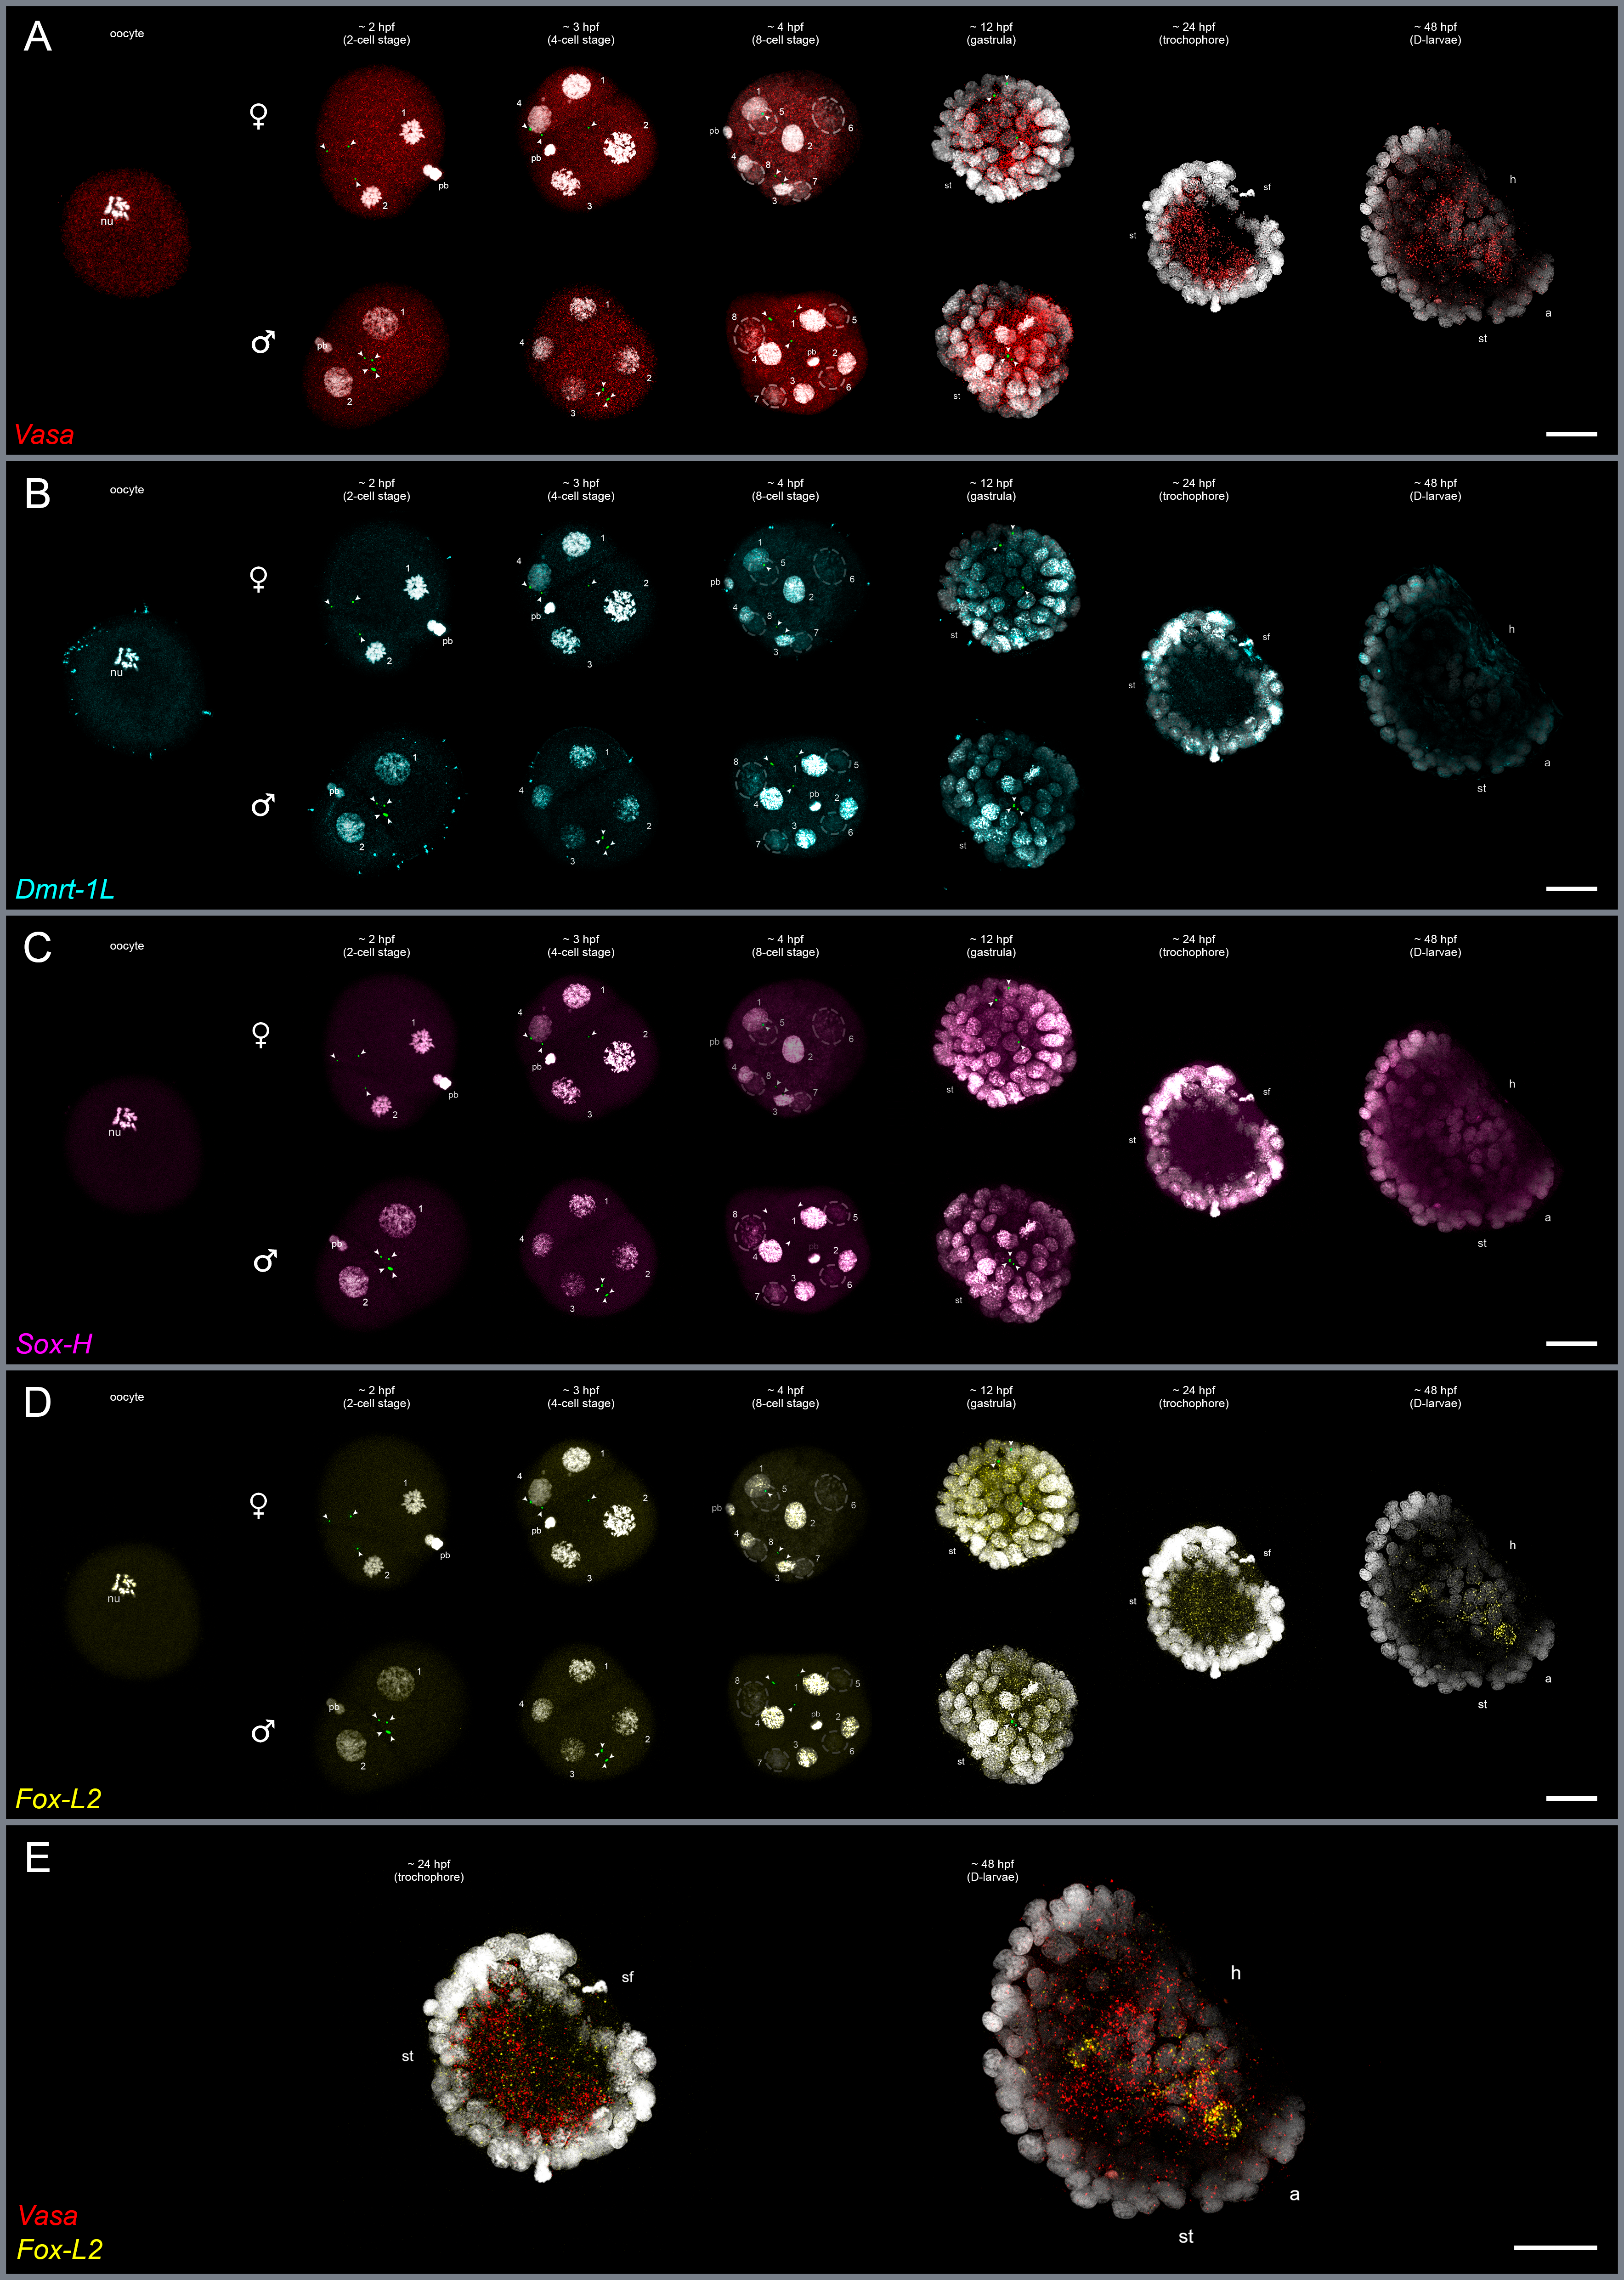
\includegraphics[width=\textwidth]{chapter_inSitu/figure_3.png}
    \caption{\textit{Caption on next page.}}
    \label{fig:hcr}
\end{figure}

\begingroup
\captionsetup[figure]{format=hruleformat}
\begin{figure}\ContinuedFloat
    \caption[]
	{
		\textbf{mRNA \textit{in-situ} \gls{hcr} of \textit{Vasa} (A), \gls{dmrt-1l} (B), \textit{Sox-H} (C), \textit{Fox-L2} (D), and \textit{Vasa}+\textit{Fox-L2} (merged; E) in several developmental stages of \gls{mgal}}. Nuclei are shown in white; in the 2-, 4-, and 8-cell stages, nuclei are also marked with numbers; in the 8-cell stage, nuclei of blastomeres in the background are highlighted with dashed circles. Sperm mitochondria, when stained (shown in green), are marked with arrowheads. For 2-cell, 4-cell, 8-cell, and gastrula stages, embryos of both sexes are reported (top rows: females; bottom rows: males). a: anus; h: hinge; nu: oocyte nucleus; pb: polar body; sf: shell field; st: stomodeum. Scale bar: \qty{20}{\um}. \textit{(Figure on previous page.)}
	}
\end{figure}
\endgroup

\subsection{Immunolocalization of Vasa}
To determine whether the commercial polyclonal antibody (ab209710 by Abcam Limited) could successfully bind \gls{mgal} Vasa, we conducted a phylogenetic analysis (\cref{fig:vasaTree-A}) and a multiple sequence alignment inspection (\cref{fig:vasaTree-B}) of Vasa/Ddx4 proteins, along with its paralog Ddx3, starting from the bivalve curated genome and transcriptome dataset analysed in \cref{chapter:molecularEvolution}. We retrieved three different Vasa sequences in the \gls{mgal} genome (\cref{suppTab:vasa_dataset}). Two of them (VDI03911.1 and VDI03912.1) are splicing variants of the same mRNA (acc. no. 10B017427) investigated through \gls{dge} and mRNA \textit{in-situ} \gls{hcr} in previous sections. Both variants are constituted by 17 exons and differ from each other for only eight leading amino acids at the protein N-terminus (\cref{fig:vasaTree-C}). Their \gls{dead/deah-box} and C-terminal domains show high levels of sequence conservation with respect to \gls{drer} Vasa (\cref{fig:vasaTree-C}). Concerning the other Vasa \gls{mgal} sequence (VDI58335.1), it originates from a separate genomic locus and appears very short (105 amino acid positions) if compared to other Vasa from bivalves (\num{> 800}; data not shown). Additionally, it does not exhibit any complete \gls{dead/deah-box} domain (as per CDD domain annotation). This considered, the additional Vasa gene (and its relative protein) may be an artefact due to genome mis-assembly and/or mis-annotation, or a non-functional gene. Thus, we argue that the correct immunolocalization of the \gls{mgal} Vasa proteins should not be affected, and will not be further discussed.

\begin{figure}
	\centering
	\captionsetup[subfigure]{labelformat=nocaption}
	\begin{subfigure}{0\linewidth}
	\caption{}\label{fig:vasaTree-A}
	\end{subfigure}% <----- get rid of space, for proper centering
	\begin{subfigure}{0\linewidth}
    \caption{}\label{fig:vasaTree-B}
    \end{subfigure}% <----- get rid of space, for proper centering
    \begin{subfigure}{0\linewidth}
    \caption{}\label{fig:vasaTree-C}
    \end{subfigure}% <----- get rid of space, for proper centering
    \includegraphics[width=\textwidth]{chapter_inSitu/figure_4.png}
	\caption[\textbf{\gls{pca} of DESeq2-normalised read counts (A) and transcription levels of target and reference genes (B)}]
	{
		\textbf{\gls{ml} phylogenetic tree of Vasa/Ddx3 and Ddx4 proteins from bivalves and reference species (A), along with the amino acid alignment of the relative \gls{dead/deah-box} (B) and of Vasa proteins from \gls{mgal} and reference species (C)}. (A) The tree has been rooted considering the Ddx4 clade as the outgroup. Reference genes from \gls{drer}, \gls{hsap}, \gls{mmus}, \gls{dmel}, and \gls{cele} are marked with an asterisk at the beginning of the tip. Bootstrap values are shown for each node. (B) The alignment of the \gls{dead/deah-box} is shown for each tip. The signature DEAD (Asp-Glu-Ala-Asp) motif can be found at positions 198--201. Vasa sequences from \gls{mgal} are highlighted with a solid rectangle and two asterisks on the right. (C) The alignment of complete Vasa sequences from \gls{mgal}, \gls{drer}, \gls{hsap}, and \gls{dmel} is shown. \gls{cele} has not been included because the species has multiple Vasa orthologs. The signature \gls{dead/deah-box} and C-terminal-associated domains are highlighted with solid rectangles. Note that position coordinates are not the same between (B) and (C). Colours of amino acid residues in both (B) and (C) correspond to the \singlecurlyquotes{Chemistry\_AA} scheme from the R package \singlecurlyquotes{ggmsa}, which highlights the amino acid side-chain chemistry (\citebold{zhou2022ggmsa}). Bivalve species IDs as in \cref{suppTab:bivalve_dataset}. Cele: \glsxtrlong{cele}; Drer: \glsxtrlong{drer}; Dmel: \glsxtrlong{dmel}; Hsap: \glsxtrlong{hsap}; Mmus: \glsxtrlong{mmus}. Full descriptions of gene names, accession numbers, and species can be found in \cref{suppTab:vasa_dataset}.

	}
	\label{fig:vasaTree}
\end{figure}

Unfortunately, the amount of available samples and antibodies for the experiment was limited. Therefore, we managed to acquire just two oocytes, two 2-cell embryos, and one gastrula. Nonetheless, from the obtained images, we found that Vasa proteins are apparently missing from the oocytes, but can be detected at increasing levels on embryos after \qty{4}{\hpf} (\cref{fig:immuno}) and during gastrulation, with a localization matching that of Vasa mRNAs (\cref{fig:vasaTree-A}). Imaging of control samples (i.e., without primary antibody reaction) can be found in \cref{suppFig:immunoBianco}.

\begin{figure}
	\floatbox[{\capbeside\thisfloatsetup{capbesideposition={right,top},capbesidewidth=0.4\textwidth}}]{figure}[\FBwidth]
	{\includegraphics[width=0.55\textwidth]{chapter_inSitu/figure_5.png}}
	{\caption[\textbf{Immunolocalization of Vasa in \gls{mgal} oocyte and embryos}]
	{
		\textbf{Immunolocalization of Vasa in \gls{mgal} oocyte and embryos}. Nuclei are shown in white. Sperm mitochondria (in green) are marked with arrowheads. nu: oocyte nucleus; pl: polar lobe; pb: polar body; st: stomodeum. Scale bar: \qty{20}{\um}.
	}
	\label{fig:immuno}}
\end{figure}

\section{Discussion} \label{chapter:insitu-discussion}
\subsection{Sperm mitochondria are not detected after 12 hpf because of MitoTracker misincorporation or fading}\label{chapter:insitu-discussionMito}
Because of the presence of the unique \gls{dui} of mitochondria, \gls{mgal} offers a compelling system to investigate \gls{sd} during the early stages of embryogenesis. As a matter of fact, the sexual fate of an embryo appears to be established as soon as the first cleavage division, according to the dispersal pattern of sperm mitochondria (\citebold{saavedra1997mytilus,cao2004differential}), despite the two processes are not necessarily causally linked (\citebold{kenchington2009dui}): (i) if the embryo is going to develop into a female, sperm mitochondria can be found scattered across different blastomeres; (ii) if the embryo is going to develop into a male, sperm mitochondria are found aggregated all in the same blastomere (usually the macromere), being subsequently transferred to \glspl{pgc} as part of the germ plasm. Therefore, in order to be able to establish the sexual identity of embryos and link it to any differential transcriptions of \glspl{dsfg}, we labelled sperm mitochondria with MitoTracker (prior to oocyte fertilisation), and check for their dispersal patterns throughout the various sampled stages. Despite being successfully retained in developing embryos up until \qty{12}{\hpf}, the MitoTracker fluorescence was difficult to detect in later stages, and so was the mitochondrial dispersal pattern. This phenomenon may have been caused by: (i) misincorporation of MitoTracker during pre-fertilization sperm incubation (ii) MitoTracker fading after intense manipulation of samples; (iii) MitoTracker dye being incompatible with proper embryo development, i.e., labelled embryos not surviving after \qty{12}{\hpf}.
Based on previous studies showing that MitoTracker labelling of sperm mitochondria (including the relative dispersed and aggregated patterns) can be observed up until the late D-larva stage in \gls{medu} (\qty{72}{\hpf}; \citebold{cao2004differential}), we argue that (i) and (ii) are the most likely explanation for the dye not being detected in samples after \qty{12}{\hpf}, i.e., MitoTracker has not interfered with the correct development of embryos. However, it must be considered that we employed a rosamine-based MitoTracker dye (MitoTracker Red; which better resists aldehydic fixation), while \citeboldyearparent{cao2004differential} used a carbocyanine-based MitoTracker dye (MitoTracker Green). This may have determined different effects on cell vitality, thus making results not comparable to each other. As a matter of fact, despite MitoTracker dyes are life-compatible as per manufacturer\curlyapostrophe s indications, \citeboldyearparent{minamikawa1999chloromethyl} showed that rosamine-based MitoTracker dyes have photosensitising effects on cells. This means that cells labelled with MitoTracker Red may be committed to apoptosis if exposed to intense light, which induce the loss of the mitochondrial membrane potential and consequent mitochondria swelling. However, based on our experimental conditions, we argue that MitoTracker Red photosensitisation has had a minimal effect, if any, on embryo development. As a matter of fact, (i) after sperm MitoTracker staining, samples were kept in the dark throughout the entire sampling period (MitoTracker Red cytotoxicity is not evident in the dark; \citebold{minamikawa1999chloromethyl}), with limited exposure to environmental light just in correspondence with water changes; furthermore, (ii) the photosensitisation has been shown to significantly increase with light doses exceeding \qty{0.4}{\J\per\square\cm} (cell-colony mortality rate of \qtyrange{60}{80}{\percent} compared to control colonies; \citebold{minamikawa1999chloromethyl}), which is higher than typical environmental light exposure (the solar constant is measured at around \qty{1.362}{\kW\per\square\m}, equivalent to \qty{0.1367}{\J\per\square\cm\per\s}); (iii) only a little proportion of mitochondria (the 5 sperm-derived mitochondria) have been labelled with MitoTracker, while the oocyte-derived ones remained unlabelled. Altogether, we think that MitoTracker Red staining did not determine a cytotoxic effect on \gls{mgal} embryos and the consequent survival of only unlabelled embryos. Thus, we conclude that MitoTracker was not properly detected on samples older than \qty{12}{\hpf} because of misincorporation since the beginning or the dye fading. However, we acknowledge that a formal survival and vitality test should be performed on \gls{mgal} embryos marked with MitoTracker Red, in order to exclude any possible cytotoxic effect.

\subsection{Exploring the processes of SD in the \textit{M. galloprovincialis} early development}
To date, the molecular basis of bivalve \gls{sd} has been investigated mainly in adult tissues (e.g., \citebold{li2018foxl2,liang2019sox2,wang2020identification,sun2022examination,wang2022transcriptome}). As a matter of fact, considering that in many bivalve species gonads form anew at the beginning of every reproductive season from several populations of \glspl{pgc} (\citebold{filanti2021early}), it can be speculated that the sexual identity may be established in correspondence with each new gonad formation. This observation would also explain the process by which many bivalve species are capable of sex changes and sex reversal from one reproductive season to the other (\citebold{breton2018sex}). Nonetheless, animal \gls{sd} is a key developmental process often triggered soon after fertilisation and occurring throughout the early development, as can be observed for example in mammals and fruit flies (\citebold{salz2010sex,beukeboom2014evolution,richardson2023comparativeSex}). Consequently, a full understanding of \gls{sd} in bivalves needs to account also for the events taking place during embryo and larval life stages. To our best knowledge, the only investigation of bivalve \glspl{srg} during non-adult stages comes from the Pacific oyster \gls{cgig} (\citebold{naimi2009molecular}), where the transcription levels of \textit{Vasa}, \gls{dmrt-1l}, and \textit{Fox-L2} have been investigated through \gls{qrt-pcr}. In this work, however, only stages between \qty{7}{\dpf} larvae and 4-month-old spats have been tested, and a direct association of the \gls{dmrt-1l}/\textit{Fox-L2} transcription levels with \gls{sd} could not be established. As a matter of fact, sexes cannot be differentiated in oysters before the onset of gametogenesis, and thus the sex of developing embryos/larvae/spats cannot be properly established (\citebold{naimi2009molecular}).

In this work, we aimed to expand the knowledge of bivalve \gls{sd} by investigating for the first time the transcription patterns of three bivalve \gls{sdg} candidates---belonging to the \gls{dsfg} families, during the embryogenesis and early larval development of the Mediterranean mussel \gls{mgal}. This species allows to infer sex of developing embryos by tracing the sperm mitochondria distribution patterns (see \cref{chapter:insitu-introduction,chapter:insitu-discussionMito}). To this purpose, we employed an explorative investigation through a \gls{dge} analysis, and mRNA \textit{in-situ} \gls{hcr}. Our experimental setting, which included the sperm mitochondria labelling, allowed us to \textit{a-priori} establish the sex of developing embryos and larvae, and thus to link any differential transcription pattern of \glspl{dsfg} to the sexual identity.

The \gls{dge} analysis showed that the inferred transcription levels of control genes, \textit{Fox-B2} and \textit{Wnt-8a} (\cref{fig:deseq2-B}), are coherent with the ones reported by \citeboldyearparent{miglioli2024hcrMytilus}, indicating that the results obtained from other genes can be considered reliable. The low or null transcription levels of both \gls{dmrt-1l} and \textit{Sox-H} (\cref{fig:deseq2-B}) may derive from the absence of transcription itself. However, it must be taken into account that \gls{mgal} shows a mather-dependent sex ratio (\citebold{saavedra1997mytilus}), that is, the percentage of females and males in the progeny is tightly linked to the mother\curlyapostrophe s nuclear genome, while being independent from the father\curlyapostrophe s. Thus, considering that \citeboldyearparent{miglioli2024hcrMytilus} do not specify the sex-ratio of the sequenced embryo pool, the possibility that the low expression levels of \gls{dmrt-1l} and \textit{Sox-H} may be caused by some sex-biased related effect cannot be ruled out. Nonetheless, mRNA \textit{in-situ} \gls{hcr} supports also for our samples the scenario depicted by the \gls{dge} analysis, that is, the two genes are likely not transcribed, as no unambiguous signal was detected (\cref{fig:hcr}\textbf{B--C}). Concerning \gls{dmrt-1l}, we think that an additional and more thorough investigation is needed, as the confocal imaging step seemed to have been affected by autofluorescent signals coming from the embryo surface and the larval shell, and/or by a-specific binding  of probes (\cref{fig:hcr}\textbf{B}). Thus, to obtain more reliable results, a new mRNA \textit{in-situ} \gls{hcr} experiment on \gls{dmrt-1l} should be designed, possibly using a set of amplifiers and fluorophores which is different from the ones employed here (B2-647; \cref{tab:fluorescent_dyes}).

The transcription levels of \textit{Fox-L2} are opposed to those of \textit{Vasa} (see \cref{chapter:insitu-results,chapter:insitu-discussionVasa,fig:deseq2-A}): the gene is not transcribed up until about \qty{12}{\hpf}, i.e., corresponding to gastrulation; from this stage onward, the gene transcription is detected homogeneously all over the embryo, and then becomes restricted to two regions located at both sides of the D-veliger larvae (\cref{fig:hcr}\textbf{D}). In particular, in this stage of development, \textit{Fox-L2} appears to be co-localised with Vasa (\cref{fig:hcr}\textbf{E}), suggesting a role in \gls{pgc} specification and/or differentiation. No sex-biased transcription has been detected for \textit{Fox-L2}, though it must be considered that after \qty{12}{\hpf} we were not able to confidently establish the sexual identity of embryos/larvae through the localization of sperm-derived mitochondria (see \cref{chapter:insitu-discussionMito}). Thus, although it is tempting to speculate a possible role of \textit{Fox-L2} in the specification of female gonads, as proposed by \citeboldyearparent{zhang2014genomic} in \gls{cgig}, no definitive conclusions can be drawn at this time.

All considered, this work suggests two scenarios: (1) \gls{dmrt-1l}, \textit{Sox-H}, and/or \textit{Fox-L2} are truly \glspl{sdg}, or in any case are top regulators in the bivalve \gls{sd} process (as proposed by previous authors [\citebold{zhang2014genomic,li2018foxl2}] and by the comparative genomics analysis of \cref{chapter:molecularEvolution}), though in \gls{mgal} \gls{sd} (hence, their activation) does not occur in early development, but in later stages; (2) \gls{dmrt-1l}, \textit{Sox-H}, and \textit{Fox-L2} are not \glspl{sdg}, but are involved in gonad differentiation and maintenance in adult individuals. That said, the two possibilities should not be viewed as mutually exclusive. As a matter of fact, \gls{dmrt-1l}, \textit{Sox-H}, and/or \textit{Fox-L2} may be required during \gls{mgal} development for early \gls{sd}, which however occur at advanced larval/spat stages, as observed in \gls{cgig} (\gls{sd} occurs at \qtyrange{40}{60}{\dpf}; \citebold{naimi2009molecular,santerre2013oyster}), but they are also required in adults to allow \glspl{pgc} to initiate the sex-specific gonad development and differentiation at every reproductive season. As a matter of fact, a similar expression pattern has been seen for \gls{mgal} \textit{vasa}, whose transcription is detectable in \glspl{pgc} (i) at a low level during the non-reproductive season, and (ii) at a high level both in immature mussels and in the reproductive season (\citebold{obata2010PCGproliferation}). Thus, it can be speculated that the genes triggering the \gls{sd} cascade may be following similar paths.

\subsection{Primordial germ cells are specified by both preformation and epigenesis in \textit{M. galloprovincialis}}\label{chapter:insitu-discussionVasa}
The process of gonad specification (including \glspl{pgc}) in bivalves have been studied in several species, both in adults (e.g., \citebold{fabioux2004oysterAdult,obata2010PCGproliferation,filanti2021early}) and during early development (\citebold{woods1932sphaerium,fabioux2004oysterEmbryo,kakoi2008vasaSaccostrea}). In the pea clam \gls{sstr} (\citebold{woods1932sphaerium}), the specification of the germline is traced back to the unfertilized oocyte, where the germline determinants (in the form of electron-dense granules, mainly containing mitochondria) are included in an asymmetric region of the cytoplasm (the germ plasm). The zygote segmentation then segregates the germ plasm in single blastomeres, until in the gastrula it is found only in two quiescent \glspl{pgc}, which derives from the 4d blastomere (nomenclature as per \citebold{lyons2012cleavage}). In the Pacific oyster \gls{cgig} (\citebold{fabioux2004oysterEmbryo}), a similar process of \gls{pgc} formation has been described. The germline marker \textit{Vasa} is found to be maternally transmitted to the embryo and deposited in a region (the germ plasm) at the vegetal pole of the oocyte. With the onset of segmentation, \textit{Vasa} progressively segregates in single blastomeres, until it is found only in two separated cell clumps at both sides of the pericardic region in the D-larva (\cref{fig:vasaComparison-A}), where they will form \glspl{pgc}. The two cell clumps derive again from the 4d blastomere and, in adult oysters, they will periodically proliferate and migrate to the adjacent connective tissue to build gonad acini during the reproductive season (\citebold{fabioux2004oysterAdult,milani2017vasa}). A different mechanism has instead been proposed for the Japanese spiny oyster \gls{skeg} (\citebold{kakoi2008vasaSaccostrea}). Here, \textit{Vasa} is said to be transcribed all over the embryo until the 8-cell stage (data are not available on the original publication), becoming progressively more restricted to certain blastomeres only after the 50-cell stage. With gastrulation, \textit{Vasa} is detected only at the posterior mesoderm, which derives from the 4d blastomere. In the present work, in the attempt to investigate the transcription patterns of several \glspl{sdg}, we also characterised the emergence of \glspl{pgc} in the early development of \gls{mgal} by mean of Vasa/Vasa localization, thus providing an additional description of \gls{pgc} development in bivalves.

\begingroup
\captionsetup[figure]{format=hruleformat}
\begin{figure}
    \centering
    \captionsetup[subfigure]{labelformat=nocaption}
	\begin{subfigure}{0\linewidth}
	\caption{}\label{fig:vasaComparison-A}
	\end{subfigure}% <----- get rid of space, for proper centering
	\begin{subfigure}{0\linewidth}
    \caption{}\label{fig:vasaComparison-B}
    \end{subfigure}% <----- get rid of space, for proper centering
	\includegraphics[width=\textwidth]{chapter_inSitu/figure_6.png}
	\caption[\textbf{Comparison of Vasa localization (in red) during the Pacific oyster \gls{cgig} (A) and the Mediterranean mussel \gls{mgal} (B) early development}]
	{
		\textbf{Comparison of Vasa localization (in red) during the Pacific oyster \gls{cgig} (A) and the Mediterranean mussel \gls{mgal} (B) early development}. Drawings not in scale. Data of \gls{cgig} from \citeboldyearparent{fabioux2004oysterEmbryo}. Blastomere nomenclature as per \citeboldyearparent{lyons2012cleavage}. a: anus; h: hinge; st: stomodeum; sf: shell field.
	}
	\label{fig:vasaComparison}
\end{figure}
\endgroup

According to the \gls{dge} analysis, \textit{Vasa} shows a transcription pattern typical of maternal factors (\citebold{xu2018oocyte}), which are stored as transcripts in the oocytes during oogenesis and then constantly decrease throughout embryo segmentation, gastrulation and early larval development, down to undetectable levels (\cref{fig:deseq2-B}). mRNA \textit{in-situ} \gls{hcr} confirmed these results, showing that \textit{Vasa} mRNA is located all over the cytoplasm of the oocyte and in all the blastomeres up until the gastrulation stage, when cells positive to Vasa move to constitute internal cell layers; following additional morphogenetic movements, \textit{Vasa}-positive cells are eventually present only in two limited regions at both the lateral sides of the D-veliger (\cref{fig:hcr}\textbf{A}). On the contrary, immunolocalization showed a different temporal distribution pattern compared to its mRNA, revealing that Vasa does not occur in the oocyte, but that its translation begins only in the late segmentation stages of the zygote and then increases with gastrulation (\cref{fig:immuno}). This different localisation is likely the result of a delay in \textit{Vasa} mRNA translation, which is activated only during the embryo segmentation and grows with the increase of cell number. Nonetheless, this different localisation pattern of mRNA and protein may also have been determined by the differential transcription/translation of the two \textit{Vasa} splicing variants annotated in the \gls{mgal} genome, or by a non-specific binding of either the \gls{hcr} DNA probes or the primary polyclonal antibody. However, considering that the two \textit{Vasa}/Vasa variants are mostly identical, except for eight leading amino acids at the protein N-terminus (\cref{fig:vasaTree-C}), in our experiments we should have been able to target both. As a matter of fact, identifying any differential expression between the two variants would be almost impossible, either through mRNA \textit{in-situ} \gls{hcr} or immunolocalization. Accordingly, the \gls{dge} analyses failed in retrieving any dissimilarity in the transcription levels of the two splicing variants (data not shown), as the experiment was based on short-read sequencing (\citebold{miglioli2024hcrMytilus}). Regarding the \gls{hcr} probes, they have been specifically designed on the complete \textit{Vasa} mRNA spliced sequence, which has already been proven to specifically label \glspl{pgc} in a previous analysis on \gls{mgal} sub-adults and adults individuals (\citebold{obata2010PCGproliferation}). Regarding the commercial antibody, given the high sequence similarity between the Vasa proteins from \gls{mgal} and \gls{drer} (the protein used to produce the antibody; see \cref{chapter:insitu-MM}), at least in their core regions (i.e., the \gls{dead/deah-box} and the C-terminal domains; \cref{fig:vasaTree-C}), we are confident that the immunolocalization procedure correctly labelled Vasa proteins; furthermore, the same set of polyclonal antibodies has been shown to successfully target \glspl{pgc}/\glspl{gc} in another bivalve species, \gls{rphi}, and its specificity has been supported by Western blotting (\cite{filanti2021early}). We thus consider our results to be strongly reliable in the correct localization of \textit{Vasa}/Vasa.

Altogether, the present study shows a process of germline specification in the Mediterranean mussel which resembles that of \gls{skeg}, but differs from the one described in \gls{cgig} (\cref{fig:vasaComparison-A}) and \gls{sstr}. As a matter of fact, contrary to these latter two species, in \gls{mgal} \textit{Vasa} transcripts do not form any evident gradient in the oocyte and early stages of embryogenesis (until 8-cell stage), while becoming progressively more restricted to specific cell populations only later in development (cref{hcr, fig:vasaComparison-B}). Particularly, with the onset of gastrulation, \textit{Vasa}-positive cells are internalised in the developing gastrula, and \textit{Vasa} is thus retained only by the inner cell layers. Once the embryo metamorphoses into a trochophore larva, \textit{Vasa} transcripts arrange in a cup-like structure in the region opposite to the shell field (the ventral side), while in the early D-veliger \textit{Vasa} is present only in two lateral regions next to the valves. Here, \glspl{pgc} are going to form, eventually constituting two symmetrical linear clumps at the base of the dorsal mantle (\citebold{obata2010PCGproliferation}), which is going to represent the primary source of stem cells for gonad acini formation at every reproductive season (\citebold{obata2010PCGproliferation}). This mechanism is also reflected in the localization of Vasa proteins, which do not show any clear gradient in the oocyte---from which is absent, and at least up until gastrulation. Altogether, these findings suggest that in the Mediterranean mussel, \textit{Vasa}/Vasa may segregate in the \glspl{pgc} not only because of their inheritance as maternal factors (through preformation), but also in response to some external (and unknown) zygotic signal (through epigenesis). Therefore, \textit{Vasa} alone do not allow to identify the \glspl{ppgc} or the \glspl{pgc} during the earliest stages of development, as instead it has been shown in adult individuals (i.e., upon \gls{pgc} formation; \citebold{obata2010PCGproliferation}). Given that \textit{Vasa}/Vasa mark a population of cells instead of few blastomeres (those constituting the \glspl{ppgc}), Vasa may consequently play a role also in the broader field of stem cell specification during embryogenesis, as shown in the marine polychaete \gls{pdum} (\citebold{rebscher2007vasa}) and the sea urchin \gls{spur} (\citebold{voronina2008vasa}). In these two species, the germline is specified via an intermediate process relying on both preformation and epigenesis, which can be considered a \singlecurlyquotes{two-step process} (\citebold{rebscher2007vasa,kumano2015evolution}). In this model, a lineage of \glspl{psc} first segregates during early embryogenesis, and then produces \glspl{pgc} and other mesodermal somatic structures by unequal cell division. The germline markers, including \textit{Vasa}, are localised in both the \glspl{psc} and in the descendant \glspl{pgc}. A similar pattern of \textit{Vasa} localisation (i.e., ubiquitously present in oocytes and during early cleavage of the embryo, then progressively restricted to specific blastomeres) has also been shown in the snail \gls{iobs} (\citebold{swartz2008vasaIlyanessa}) and the abalone \gls{hasi} (\citebold{kranz2010vasaHaliotis}), despite not being directly linked to \gls{psc} specification.

\section{Conclusion}\label{chapter:insitu-conclusions}
In the present work, we hypothesise that the \gls{pgc} specification in \gls{mgal} follows a two-step process (i.e., a combination of both preformation and epigenesis), which involves the \glspl{pgc} to be formed only after embryogenesis (\citebold{kumano2015evolution}). A similar process may also be hypothesised for \gls{skeg} (\citebold{kakoi2008vasaSaccostrea}). This mechanism may also explain why \gls{dmrt-1l} and \textit{Sox-H}, if confirmed as \glspl{sdg}, are not transcribed during the investigated developmental stages. \gls{sd} would in fact happen only upon \gls{pgc} commitment, thus during advanced larval development. The present work also represents the first attempt to characterise the spatial localisation of three \glspl{dsfg} in the Mediterranean mussel embryonic and larval develpoment, along with \textit{Vasa}/Vasa, and proves the importance of considering also the developmental stages when investigating new species in a comparative framework. Adopting such an evolutionary developmental perspective may in fact reveal new processes and patterns in animal biology, even when considering related species. As a matter of fact, on the basis of available studies, it has been previously proposed that \gls{pgc} specification is generally based on epigenesis in gastropods and preformation in bivalves (\citebold{obata2012PCGspecification_molluscs}), even though the underlying mechanisms may be species-specific (\citebold{obata2012PCGspecification_molluscs}). However, the model represented by the Mediterranean mussel showed that the process of \gls{pgc} specification may be more diverse in bivalves than expected: preformation happens in \gls{cgig} and \gls{sstr}, and the two-step process happens instead in \gls{skeg}, and, as we propose, in \gls{mgal}. Therefore, results provided by the present work support the idea that the traditional preformation and epigenesis should not be accounted as mutually-exclusive phenomena nor as the only mechanisms of \gls{pgc} formation (\citebold{extavour2007evolutionGermline,kumano2015evolution}). Clearly, given the unavailability of any \gls{pgc} marker in bivalve embryos and larvae (and in mollusc in general), at the moment it is not possible to unambiguously establish the emergence and commitment of \glspl{pgc} during embryogenesis (\citebold{rebscher2014establishing}), especially if based only on few germline genes. As a matter of fact, \glspl{pgc} may share certain genetic markers (e.g., \textit{Vasa}, \textit{Nanos}, \textit{Piwi}, and \textit{Pl-10}) also with some stem cell lineages (\citebold{extavour2003mechanisms,extavour2007evolutionGermline,rebscher2007vasa,voronina2008vasa,rebscher2014establishing,piccinini2023germline}). Thus, more comprehensive investigations are needed to fully and unambiguously characterise the emergence of the germline in bivalve embryos, for example through the examination of the histological and cytological morphology and of genetic regulations (\citebold{extavour2003mechanisms}). A similar scenario holds true also for \gls{sd} and \glspl{sdg}. In fact, we should not expect that the sex-determining process, together with its underlying gene regulatory networks and the timing of its expression, is the same across the entire bivalve diversity. \gls{sd} is indeed one of the most variable developmental processes, despite its importance in the morphological development of an organism (\citebold{capel2017vertebrate}). However, it can be expected that the main actors, being them genetics or environmental or of multiple origin, are conserved, at least in having a role along the whole \gls{sd} process (\citebold{capel2017vertebrate}). Future studies would thus need to further address the functions of the main \gls{dsfg} candidates, as well as the modes of \gls{sd} and germline development, through cutting-edge techniques (such as single-cell RNA-sequencing) and possibly also encompassing various life stages. In this sense, it is tempting to consolidate the role of the Mediterranean mussel as a model system for \gls{sd} and germline studies by taking advantage not only of the \gls{dui} of mitochondria as a proxy for the sexual identity, but also of the ability of the species to produce a sex-biased offspring with the sole maternal influence (\citebold{saavedra1997mytilus}). This would allow a more thorough and straightforward investigation of the determinants influencing the sex and germline specification of developing mussels, by means of targeted RNA-sequencing and transcript/protein localisation.

% \end{document}

% \documentclass[../main.tex]{subfiles}

% \begin{document}

{
\setstretch{1.0}
\chapter{Conclusions}
\label{chapter:conclusions}
}

The main objective of this PhD thesis was to investigate bivalve \gls{sd} through the lens of evolutionary and integrative biology. Bivalves is a group of animals characterised by highly heterogeneous sexual and reproductive modes, with strictly gonochoristic species, obligate and facultative hermaphrodites (either protandrous, protogynous and bidirectional), as well as androgenetic systems. Both genetic and environmental factors seem to influence the sexual identity, at various degrees according to the species, and \glspl{hesc} seem to have not been selected throughout the bivalve evolutionary history. Therefore, a rigorous comparative approach is essential to unravel the extreme complexity that regulates bivalve \gls{sd}. Particularly, by combining bioinformatics with \textit{wet-lab} techniques, including genomics, phylogenetics, molecular evolution analyses, \gls{dge}, mRNA \textit{in-situ} \gls{hcr}, and immunolocalization, this work lays the foundation to understanding how \glspl{srg}, with a special focus on the \gls{dsfg} families, have evolved and may function in sex-determining processes across the bivalve taxonomic diversity.

In \cref{chapter:perspective}, the emerging role of bivalves as model organisms for \gls{sd} studies has been emphasised through a critical examination of the current knowledge. The complexity of bivalve reproduction and sexual systems underscored the need to view \gls{sd} not as a binary and stationary process, but rather as a highly dynamic continuum influenced by multiple genetic and environmental factors. Adopting this broader perspective will allow for a more effective investigation of the biology of \gls{sd}.

In \cref{chapter:molecularEvolution}, the molecular evolution of \glspl{srg} across a range of bivalve species was analysed. The findings revealed patterns of accelerated \gls{aasd} in key \glspl{srg}, namely \gls{dmrt-1l} and \textit{Sox-H}, supporting the hypothesis that these genes are deeply involved in \gls{sd} mechanisms, possibly even as primary \glspl{sdg}. Thanks to a comparative study which encompassed the analysis of additional control datasets---mammals and \textit{Drosophila}, the validity of the results has been confirmed and discussed in the light of a broader framework. This comparative approach allowed for the identification of evolutionary convergences and divergences, advancing our understanding of the patterns of molecular evolution in animal \glspl{srg}.

\cref{chapter:insitu} focused on gene expression studies in the Mediterranean mussel \gls{mgal}, offering insights into the \gls{sd} process in early development. Particularly, \gls{dmrt-1l} and \textit{Sox-H} appear to not be expressed during these stages, while \textit{Fox-L2} transcription starts only with the onset of gastrulation. This suggests that either these genes are not top regulators of \gls{sd}, or that \gls{sd} occurs only later in development, thus their expression is not found during the analysed stages. The latter interpretation would be in line with the pattern of \gls{pgc} specification in \gls{mgal}, which begins only in correspondence with the onset of gastrulation, thus not following a strict preformation model as in other studied bivalves.

Overall, this thesis further demonstrates that bivalves, with their vast reproductive and sexual diversity, serve as ideal models for investigating the complexity of \gls{sd}. By integrating genomic analyses with developmental biology, this work provides a new framework for understanding how \gls{srg} evolve and function in diverse species. Future studies could build on these insights by exploring the functional roles of \glspl{srg} through other advanced techniques (such as CRISPR-Cas9), thus expanding our understanding of the genetic underpinnings of \gls{sd} and differentiation. This integrative approach has the potential to unlock new knowledge not only in bivalves but across a wide array of species, deepening our understanding of the evolutionary forces shaping reproductive biology in animals.

% end{document}

% bibliography
\begin{refcontext}[sorting=nyt]
	\printbibliography[title=References]
	\addcontentsline{toc}{chapter}{References}
\end{refcontext}

% appendix and supp matherials
% \documentclass[../main.tex]{subfiles}

% \begin{document}

{
\chapter*{\vspace{-3cm}Appendix}
\addcontentsline{toc}{chapter}{Appendix}
\label{appendix}
}

The appendix includes the titles and abstracts of the papers published during my PhD that are not part of this thesis.

\clearpage

%----------------------------------------------------------------------------------

{
\setstretch{0.8}
\section*{\LARGE{Taxonomic revision of the Australian stick insect genus \textit{Candovia} (Phasmida: Necrosciinae): insight from molecular systematics and species-delimitation approaches.}}

\vspace{5mm}

\noindent{\Large{Giobbe Forni\textsuperscript{1,2}, Alex Cussigh\textsuperscript{1,2}, Paul D. Brock\textsuperscript{3}, Braxton R. Jones\textsuperscript{4}, Filippo Nicolini\textsuperscript{1}, Jacopo Martelossi\textsuperscript{1}, Andrea Luchetti\textsuperscript{1}}, Barbara \\ Mantovani\textsuperscript{1}}

\vspace{5mm}

\noindent{\textsuperscript{1}\textit{Department of Biological, Geological and Environmental Sciences, University of Bologna, Bologna, Italy}.}

\noindent{\textsuperscript{2}\textit{Department of Agricultural and Environmental Sciences, University of Milan, Milano, Italy}.}

\noindent{\textsuperscript{3}\textit{The Natural History Museum, Cromwell Road, London, UK}.}

\noindent{\textsuperscript{4}\textit{School of Life and Environmental Sciences, The University of Sydney, Sydney NSW 2006, Australia}.}

\vspace{5mm}

\noindent{\large{\textbf{Published in}: 2023, \textit{Zoological Journal of the Linnean Society}, 197:189--210. \hfill \\ \href{https://doi.org/10.1093/zoolinnean/zlac074}{10.1093/zoolinnean/zlac074}}}
}

\vspace{5mm}

\textbf{Abstract}. The Phasmida genus \textit{Candovia} comprises nine traditionally recognized species, all endemic to Australia. In this study, \textit{Candovia} diversity is explored through molecular species-delimitation analyses using the \textit{COI\textsubscript{Fol}} gene fragment and phylogenetic inferences leveraging seven additional mitochondrial and nuclear loci. Molecular results were integrated with morphological observations, leading us to confirm the already described species and to the delineation of several new taxa and of the new genus \textit{Paracandovia}. New \textit{Candovia} species from various parts of Queensland and New South Wales are described and illustrated (\textit{C. alata} sp. nov., \textit{C. byfieldensis} sp. nov., \textit{C. dalgleishae} sp. nov., \textit{C. eungellensis} sp. nov., \textit{C. karasi} sp. nov., \textit{C. koensi} sp. nov. and \textit{C. wollumbinensis} sp. nov.). New combinations are proposed and species removed from synonymy with the erection of the new genus \textit{Paracandovia} (\textit{P. cercata} stat. rev., comb. nov., \textit{P. longipes} stat. rev., comb. nov., \textit{P. pallida} comb. nov., \textit{P. peridromes} comb. nov., \textit{P. tenera} stat. rev., comb. nov.). Phylogenetic analyses suggest that the egg capitulum may have independently evolved multiple times throughout the evolutionary history of these insects. Furthermore, two newly described species represent the first taxa with fully developed wings in this previously considered apterous clade.

\clearpage

%----------------------------------------------------------------------------------

{
\setstretch{1.0}
\section*{\LARGE{Comparative genomics of \textit{Hox} and \textit{ParaHox} \\ genes among major lineages of Branchiopoda with emphasis on tadpole shrimps.}}

\vspace{5mm}

\noindent{\Large{Filippo Nicolini\textsuperscript{1,2}, Jacopo Martelossi\textsuperscript{1}, Giobbe Forni\textsuperscript{3}, \\ Castrense Savojardo\textsuperscript{4}, Barbara Mantovani\textsuperscript{1}, Andrea Luchetti\textsuperscript{1}}}

\vspace{5mm}

\noindent{\textsuperscript{1}\textit{Department of Biological, Geological and Environmental Sciences, University of Bologna, Bologna, Italy}.}

\noindent{\textsuperscript{2}\textit{Fano Marine Center, Fano (PU), Italy}.}

\noindent{\textsuperscript{3}\textit{Department of Agricultural and Environmental Sciences, University of Milan, Milan, Italy}.}

\noindent{\textsuperscript{4}\textit{Department of Pharmacy and Biotechnology, University of Bologna, Bologna, Italy}.}

\vspace{5mm}

\noindent{\large{\textbf{Published in}: 2023, \textit{Frontiers in Ecology and Evolution}, 11:1046960. \hfill \\ \href{https://doi.org/10.3389/fevo.2023.1046960}{10.3389/fevo.2023.1046960}}}
}

\vspace{5mm}

\textbf{Abstract}. \textit{Hox} and \textit{ParaHox} genes (HPHGs) are key developmental genes that pattern regional identity along the anterior–posterior body axis of most animals. Here, we identified HPHGs in tadpole shrimps (Pancrustacea, Branchiopoda, Notostraca), an iconic example of the so-called “living fossils” and performed a comparative genomics analysis of HPHGs and the \textit{Hox} cluster among major branchiopod lineages. Notostraca possess the entire \textit{Hox} complement, and the \textit{Hox} cluster seems to be split into two different subclusters, although we were not able to support this finding with chromosome-level assemblies. However, the genomic structure of \textit{Hox} genes in Notostraca appears more derived than that of \textit{Daphnia} spp., which instead retains the plesiomorphic condition of a single compact cluster. Spinicaudata and \textit{Artemia franciscana} show instead a \textit{Hox} cluster subdivided across two or more genomic scaffolds with some orthologs either duplicated or missing. Yet, branchiopod HPHGs are similar among the various clades in terms of both intron length and number, as well as in their pattern of molecular evolution. Sequence substitution rates are in fact generally similar for most of the branchiopod \textit{Hox} genes and the few differences we found cannot be traced back to natural selection, as they are not associated with any signals of diversifying selection or substantial switches in selective modes. Altogether, these findings do not support a significant stasis in the Notostraca \textit{Hox} cluster and further confirm how morphological evolution is not tightly associated with genome dynamics.

\clearpage

%----------------------------------------------------------------------------------

{
\setstretch{1.0}
\section*{\LARGE{Multiple and diversified transposon lineages contribute to early and recent bivalve genome evolution.}}

\vspace{5mm}

\noindent{\Large{Jacopo Martelossi\textsuperscript{1}, Filippo Nicolini\textsuperscript{1,2}, Simone Subacchi\textsuperscript{1}, Daniela \\ Pasquale\textsuperscript{1}, Fabrizio Ghiselli\textsuperscript{1}, Andrea Luchetti\textsuperscript{1}}}

\vspace{5mm}

\noindent{\textsuperscript{1}\textit{Department of Biological, Geological and Environmental Sciences, University of Bologna, Bologna, Italy}.}

\noindent{\textsuperscript{2}\textit{Fano Marine Center, Fano (PU), Italy}.}

\vspace{5mm}

\noindent{\large{\textbf{Published in}: 2023, \textit{BMC Biology}, 21:145. \hfill \\ \href{https://doi.org/10.1186/s12915-023-01632-z}{10.1186/s12915-023-01632-z}}}
}

\vspace{5mm}

\textbf{Abstract}. \textbf{Background}. Transposable elements (TEs) can represent one of the major sources of genomic variation across eukaryotes, providing novel raw materials for species diversification and innovation. While considerable effort has been made to study their evolutionary dynamics across multiple animal clades, molluscs represent a substantially understudied phylum. Here, we take advantage of the recent increase in mollusc genomic resources and adopt an automated TE annotation pipeline combined with a phylogenetic tree-based classification, as well as extensive manual curation efforts, to characterize TE repertories across 27 bivalve genomes with a particular emphasis on DDE/D class II elements, long interspersed nuclear elements (LINEs), and their evolutionary dynamics. \textbf{Results}. We found class I elements as highly dominant in bivalve genomes, with LINE elements, despite less represented in terms of copy number per genome, being the most common retroposon group covering up to 10\% of their genome. We mined 86,488 reverse transcriptases (RVT) containing LINE coming from 12 clades distributed across all known superfamilies and 14,275 class II DDE/D-containing transposons coming from 16 distinct superfamilies. We uncovered a previously underestimated rich and diverse bivalve ancestral transposon complement that could be traced back to their most recent common ancestor that lived about 500 Mya. Moreover, we identified multiple instances of lineage-specific emergence and loss of different LINEs and DDE/D lineages with the interesting cases of CR1-Zenon, Proto2, RTE-X, and Academ elements that underwent a bivalve-specific amplification likely associated with their diversification. Finally, we found that this LINE diversity is maintained in extant species by an equally diverse set of long-living and potentially active elements, as suggested by their evolutionary history and transcription profiles in both male and female gonads. \textbf{Conclusions}. We found that bivalves host an exceptional diversity of transposons compared to other molluscs. Their LINE complement could mainly follow a “stealth drivers” model of evolution where multiple and diversified families are able to survive and co-exist for a long period of time in the host genome, potentially shaping both recent and early phases of bivalve genome evolution and diversification. Overall, we provide not only the first comparative study of TE evolutionary dynamics in a large but understudied phylum such as Mollusca, but also a reference library for ORF-containing class II DDE/D and LINE elements, which represents an important genomic resource for their identification and characterization in novel genomes.

\clearpage

%----------------------------------------------------------------------------------

{
\setstretch{1.0}
\section*{\LARGE{Towards a time-tree solution for Branchiopoda diversification: a jackknife assessment of fossil age priors.}}

\vspace{5mm}

\noindent{\Large{Niccolò Righetti\textsuperscript{1}*, Filippo Nicolini\textsuperscript{2}*, Giobbe Forni\textsuperscript{2}, Andrea Luchetti\textsuperscript{2}}}

\vspace{5mm}

\noindent{\textsuperscript{1}\textit{Laboratoire de Biologie Computationnelle et Quantitative (LCQB), Sorbonne Université, CNRS, IBPS, UMR7238, Paris, France}.}

\noindent{\textsuperscript{2}\textit{Department of Biological, Geological and Environmental Sciences, University of Bologna, Bologna, Italy}.}

\noindent{* the authors equally contributed to this work.}

\vspace{5mm}

\noindent{\large{\textbf{\textit{Submitted for peer-review.}}}}
}

\vspace{5mm}

\textbf{Abstract}. An understanding of Branchiopoda's evolutionary history is crucial for a comprehensive knowledge of the Pancrustacea tree of life, given their close evolutionary relationship with Hexapoda. Despite significant advances in molecular and morphological phylogenetics that have resolved much of the branchiopod backbone topology, a reliable temporal framework remains elusive. Key challenges include a sparse fossil record, long-term morphological stasis, and past topological inconsistencies. Leveraging a Bayesian Inference approach and the most extensive phylogenomic dataset for branchiopod to date, encompassing 46 species and over 130 genes, we inferred a time-calibrated phylogenetic tree. Furthermore, to strengthen the confidence in our divergence times estimation, we assessed the impact of age priors, topological uncertainties, and gene trees which are discordant from the species trees. Our results are largely consistent with the fossil record and with previous studies, indicating that Branchiopoda originated between 400 and 500 million years ago, and the orders of large branchiopods diversified during the Mesozoic. Concerning Cladocera, results remain problematic, with a sharper uncertainty in the diversification time with respect to the fossil record. Though, the jackknife resampling of fossils and the other sensitivity analyses proved our calibration method to be robust, suggesting that the difficulties in obtaining a paleontological-consistent time tree may be hindered by the variability in branchiopod substitution rates and topological instability within certain clades.

% \end{document}
% \documentclass[../main.tex]{subfiles}

% \begin{document}

{
\setstretch{1.0}
\chapter*{Supplementary figures}
\addcontentsline{toc}{chapter}{Supplementary figures}
\label{supp_fig}
\markboth{Supplementary figures}{Supplementary figures}
}

High-quality supplementary figures are available at the following GitHub repository:

\ulhref{https://github.com/filonico/phd_thesis_tex}{https://github.com/filonico/phd\_thesis\_tex}

\setcounter{figure}{0}
\renewcommand{\figurename}{Supplementary Figure}
\renewcommand{\thefigure}{\textbf{S\arabic{figure}}}

\begin{figure}[ht]
	\centering
	\includegraphics[width=0.7\textwidth]{supp_figures/supp_fig_S1.pdf}
	\caption[\textbf{\gls{ml} phylogenetic tree of the Dmrt gene family in molluscs, including the possvm orthology inference}]
	{
		\textbf{\gls{ml} phylogenetic tree of the Dmrt gene family in molluscs, including the possvm orthology inference}. Reference genes from \gls{hsap}, \gls{cele}, and \gls{dmel} are marked with an asterisk at the beginning of the tip names. Species ID can be found in \cref{suppTab:bivalve_dataset}. The tree has been midpoint rooted. Bootstrap values are shown for each node.
	}
	\label{suppFig:dmrt_bivalves}
\end{figure}

\begin{figure}[ht]
	\centering
	\includegraphics[height=0.9\textheight]{supp_figures/supp_fig_S2.pdf}
	\caption[\textbf{\gls{ml} phylogenetic tree of the Sox gene family in molluscs, including the possvm orthology inference}]
	{
		\textbf{\gls{ml} phylogenetic tree of the Sox gene family in molluscs, including the possvm orthology inference}. Reference genes from \gls{hsap}, \gls{cele}, and \gls{dmel} are marked with an asterisk at the beginning of the tip names. Species ID can be found in \cref{suppTab:bivalve_dataset}. Bootstrap values are shown for each node.
	}
	\label{suppFig:sox_bivalves}
\end{figure}

\begin{figure}[ht]
	\centering
	\includegraphics[height=0.9\textheight]{supp_figures/supp_fig_S3.pdf}
	\caption[\textbf{\gls{ml} phylogenetic tree of the Fox gene family in molluscs, including the possvm orthology inference}]
	{
		\textbf{\gls{ml} phylogenetic tree of the Fox gene family in molluscs, including the possvm orthology inference}. Reference genes from \gls{hsap}, \gls{cele}, and \gls{dmel} are marked with an asterisk at the beginning of the tip names. Species ID can be found in \cref{suppTab:bivalve_dataset}. Bootstrap values are shown for each node.
	}
	\label{suppFig:fox_bivalves}
\end{figure}

\begin{figure}[ht]
	\centering
	\includegraphics[width=0.95\textwidth]{supp_figures/supp_fig_S4.png}
	\captionsetup[subfigure]{labelformat=nocaption}
	\begin{subfigure}{0\linewidth}
		\caption{}\label{suppFig:DSFG_testCompilation-A}
	\end{subfigure}% <----- get rid of space, for proper centering
	\begin{subfigure}{0\linewidth}
		\caption{}\label{suppFig:DSFG_testCompilation-B}
	\end{subfigure}% <----- get rid of space, for proper centering
	\caption[\textbf{The DSFG complement in Mammalia and \textit{Drosophila} spp.}]
	{
		\textbf{The DSFG complement in Mammalia (A) and \textit{Drosophila} spp. (B)}. Presence/absence of genes in various species are indicated by filled circles. Numbers inside each circle specify genes with 2 or more copies. The shaded area highlights outgroup species, \gls{ggal} (Aves) for mammals and \gls{agam} (Culicidae) for fruit flies. The phylogenetic tree of analysed species, as inferred from literature, is shown on the left, while major taxonomic groups are reported on the right. All species are represented by genomic data. \gls{dsfg} trees are shown on the bottom (full trees can be found in \cref{suppFig:dmrt_mammals,suppFig:fox_mammals}). Full species names for both mammals and fruit flies, along with all assembly and taxonomic information, can be found in \cref{suppTab:mammal_dataset,suppTab:drosophila_dataset}, respectively. A.: Aves; Chirop.: Chiroptera; L.: Lagomorpha; M.: Monotremata; Me.: Metatheria; P.: Pholidota; Pe.: Perissodactyla; Prim.: Primates; Roden.: Rodentia; X.: Xenarthra; C.: Culicidae.
	}
	\label{suppFig:DSFG_testCompilation}
\end{figure}

\begin{figure}[ht]
	\centering
	\includegraphics[height=0.85\textheight]{supp_figures/supp_fig_S5.pdf}
	\caption[\textbf{\gls{ml} phylogenetic tree of the \gls{dmrt} gene family in mammals, including the Possvm orthology inference}]
	{
		\textbf{\gls{ml} phylogenetic tree of the \gls{dmrt} gene family in mammals, including the Possvm orthology inference}. Reference genes from \gls{hsap}, \gls{mmus}, \gls{emax}, and \gls{oana} are marked with an asterisk at the beginning of the tip names. Species ID can be found in \cref{suppTab:mammal_dataset}. The tree has been midpoint rooted. Bootstrap values are shown for each node.
	}
	\label{suppFig:dmrt_mammals}
\end{figure}

\begin{figure}[ht]
	\centering
	\includegraphics[height=0.85\textheight]{supp_figures/supp_fig_S6.pdf}
	\caption[\textbf{\gls{ml} phylogenetic tree of the \gls{sox} gene family in mammals, including the Possvm orthology inference}]
	{
		\textbf{\gls{ml} phylogenetic tree of the \gls{sox} gene family in mammals, including the Possvm orthology inference}. Reference genes from \gls{hsap}, \gls{mmus}, \gls{emax}, and \gls{oana} are marked with an asterisk at the beginning of the tip names. Species ID can be found in \cref{suppTab:mammal_dataset}. Bootstrap values are shown for each node.
	}
	\label{suppFig:sox_mammals}
\end{figure}

\begin{figure}[ht]
	\centering
	\includegraphics[height=0.85\textheight]{supp_figures/supp_fig_S7.pdf}
	\caption[\textbf{\gls{ml} phylogenetic tree of the \gls{fox} gene family in mammals, including the Possvm orthology inference}]
	{
		\textbf{\gls{ml} phylogenetic tree of the \gls{fox} gene family in mammals, including the Possvm orthology inference}. Reference genes from \gls{hsap}, \gls{mmus}, \gls{emax}, and \gls{oana} are marked with an asterisk at the beginning of the tip names. Species ID can be found in \cref{suppTab:mammal_dataset}. Bootstrap values are shown for each node.
	}
	\label{suppFig:fox_mammals}
\end{figure}

\begin{figure}[ht]
	\centering
	\includegraphics[width=\textwidth]{supp_figures/supp_fig_S8.pdf}
	\caption[\textbf{\gls{ml} phylogenetic tree of the \gls{dmrt} gene family in fruit flies, including the Possvm orthology inference}]
	{
		\textbf{\gls{ml} phylogenetic tree of the \gls{dmrt} gene family in fruit flies, including the Possvm orthology inference}. Reference genes from \gls{dmel}, \gls{dhyd}, \gls{dpse}, and \gls{dsuz} are marked with an asterisk at the beginning of the tip names. Species ID can be found in \cref{suppTab:drosophila_dataset}. The tree has been midpoint rooted. Bootstrap values are shown for each node.
	}
	\label{suppFig:dmrt_drosophila}
\end{figure}

\begin{figure}[ht]
	\centering
	\includegraphics[width=\textwidth]{supp_figures/supp_fig_S9.pdf}
	\caption[\textbf{\gls{ml} phylogenetic tree of the \gls{sox} gene family in fruit flies, including the Possvm orthology inference}]
	{
		\textbf{\gls{ml} phylogenetic tree of the \gls{sox} gene family in fruit flies, including the Possvm orthology inference}. Reference genes from \gls{dmel}, \gls{dhyd}, \gls{dpse}, and \gls{dsuz} are marked with an asterisk at the beginning of the tip names. Species ID can be found in \cref{suppTab:drosophila_dataset}. Bootstrap values are shown for each node.
	}
	\label{suppFig:sox_drosophila}
\end{figure}

\begin{figure}[ht]
	\centering
	\includegraphics[width=\textwidth]{supp_figures/supp_fig_S10.pdf}
	\caption[\textbf{\gls{ml} phylogenetic tree of the \gls{fox} gene family in fruit flies, including the Possvm orthology inference}.]
	{
		\textbf{\gls{ml} phylogenetic tree of the \gls{fox} gene family in fruit flies, including the Possvm orthology inference}. Reference genes from \gls{dmel}, \gls{dhyd}, \gls{dpse}, and \gls{dsuz} are marked with an asterisk at the beginning of the tip names. Species ID can be found in \cref{suppTab:drosophila_dataset}. Bootstrap values are shown for each node.
	}
	\label{suppFig:fox_drosophila}
\end{figure}

\begin{figure}[ht]
	\centering
	\includegraphics[width=\textwidth]{supp_figures/supp_fig_S11.pdf}
	\caption[\textbf{\gls{ml} phylogenetic tree of the \gls{dmrt} gene family in mollusc species}]
	{
		\textbf{\gls{ml} phylogenetic tree of the \gls{dmrt} gene family in mollusc species}. Species ID can be found in \cref{suppTab:bivalve_dataset}. The tree has been midpoint rooted. Bootstrap values are shown for each node.
	}
	\label{suppFig:dmrt_molluscOnly}
\end{figure}

\begin{figure}[ht]
	\centering
	\includegraphics[width=\textwidth]{supp_figures/supp_fig_S12.pdf}
	\caption[\textbf{\gls{ml} phylogenetic tree of \textit{Sox-B1} and \textit{Sox-B2} genes in mollusc and reference species}]
	{
		\textbf{\gls{ml} phylogenetic tree of \textit{Sox-B1} and \textit{Sox-B2} genes in mollusc and reference species}. Reference genes from \gls{hsap}, \gls{cele}, and \gls{dmel} are marked with an asterisk at the beginning of the tip names. Species ID can be found in \cref{suppTab:bivalve_dataset}. Bootstrap values are shown for each node.
	}
	\label{suppFig:sox_B12}
\end{figure}

\begin{figure}[ht]
	\centering
	\includegraphics[height=0.85\textheight]{supp_figures/supp_fig_S13.pdf}
	\caption[\textbf{ML phylogenetic tree of \textit{Fox-J2}, \textit{Fox-M}, \textit{Fox-O}, and \textit{Fox-P} genes in mollusc and reference species}]
	{
		\textbf{ML phylogenetic tree of \textit{Fox-J2}, \textit{Fox-M}, \textit{Fox-O}, and \textit{Fox-P} genes in mollusc and reference species}. Reference genes from \textit{H. sapiens}, \textit{C. elegans}, and \textit{D. melanogaster} are marked with an asterisk at the beginning of the tip names. Species ID can be found in \cref{suppTab:bivalve_dataset}. Bootstrap values are shown for each node.
	}
	\label{suppFig:fox_JMOP}
\end{figure}

\begin{figure}[ht]
	\centering
	\includegraphics[height=0.85\textheight]{supp_figures/supp_fig_S14.pdf}
	\caption[\textbf{\gls{ml} phylogenetic tree of the Fox gene family in bivalves and the sea urchin \gls{spur} (Spur)}]
	{
		\textbf{\gls{ml} phylogenetic tree of the Fox gene family in bivalves and the sea urchin \gls{spur} (Spur)}. Reference genes from \gls{spur} are marked with an asterisk at the beginning of the tip names. Species ID can be found in \cref{suppTab:bivalve_dataset}. \gls{spur} genes are those given by \citebold{tu2006sea}. Bootstrap values are shown for each node.
	}
	\label{suppFig:fox_spur}
\end{figure}

\begin{figure}[ht]
	\centering
	\includegraphics[width=\textwidth]{supp_figures/supp_fig_S15.png}
	\caption[\textbf{Distribution of \gls{aasd} of single-copy orthogroups in \gls{cgig}, \gls{cang}, \gls{cari}, and \gls{cvir} (A), including \gls{dsfg} (B)}]
	{
		\textbf{Distribution of \gls{aasd} of single-copy orthogroups in \gls{cgig}, \gls{cang}, \gls{cari}, and \gls{cvir} (A), including \gls{dsfg} (B)}. The distribution of \gls{aasd} in \textit{Crassostrea} has been computed on the median values of pairwise distances of over \qty{14}{\kilo\nothing} \glspl{sco}. Circle heights of \glspl{dsfg} show the median value of their \gls{aasd}. \textit{Dmrt-1L} genes are indicated as ‘dmrt\_disco\_tree3’.
	}
	\label{suppFig:DSFG_crassostreaDivergence}
\end{figure}

\begin{figure}[ht!]
	\centering
	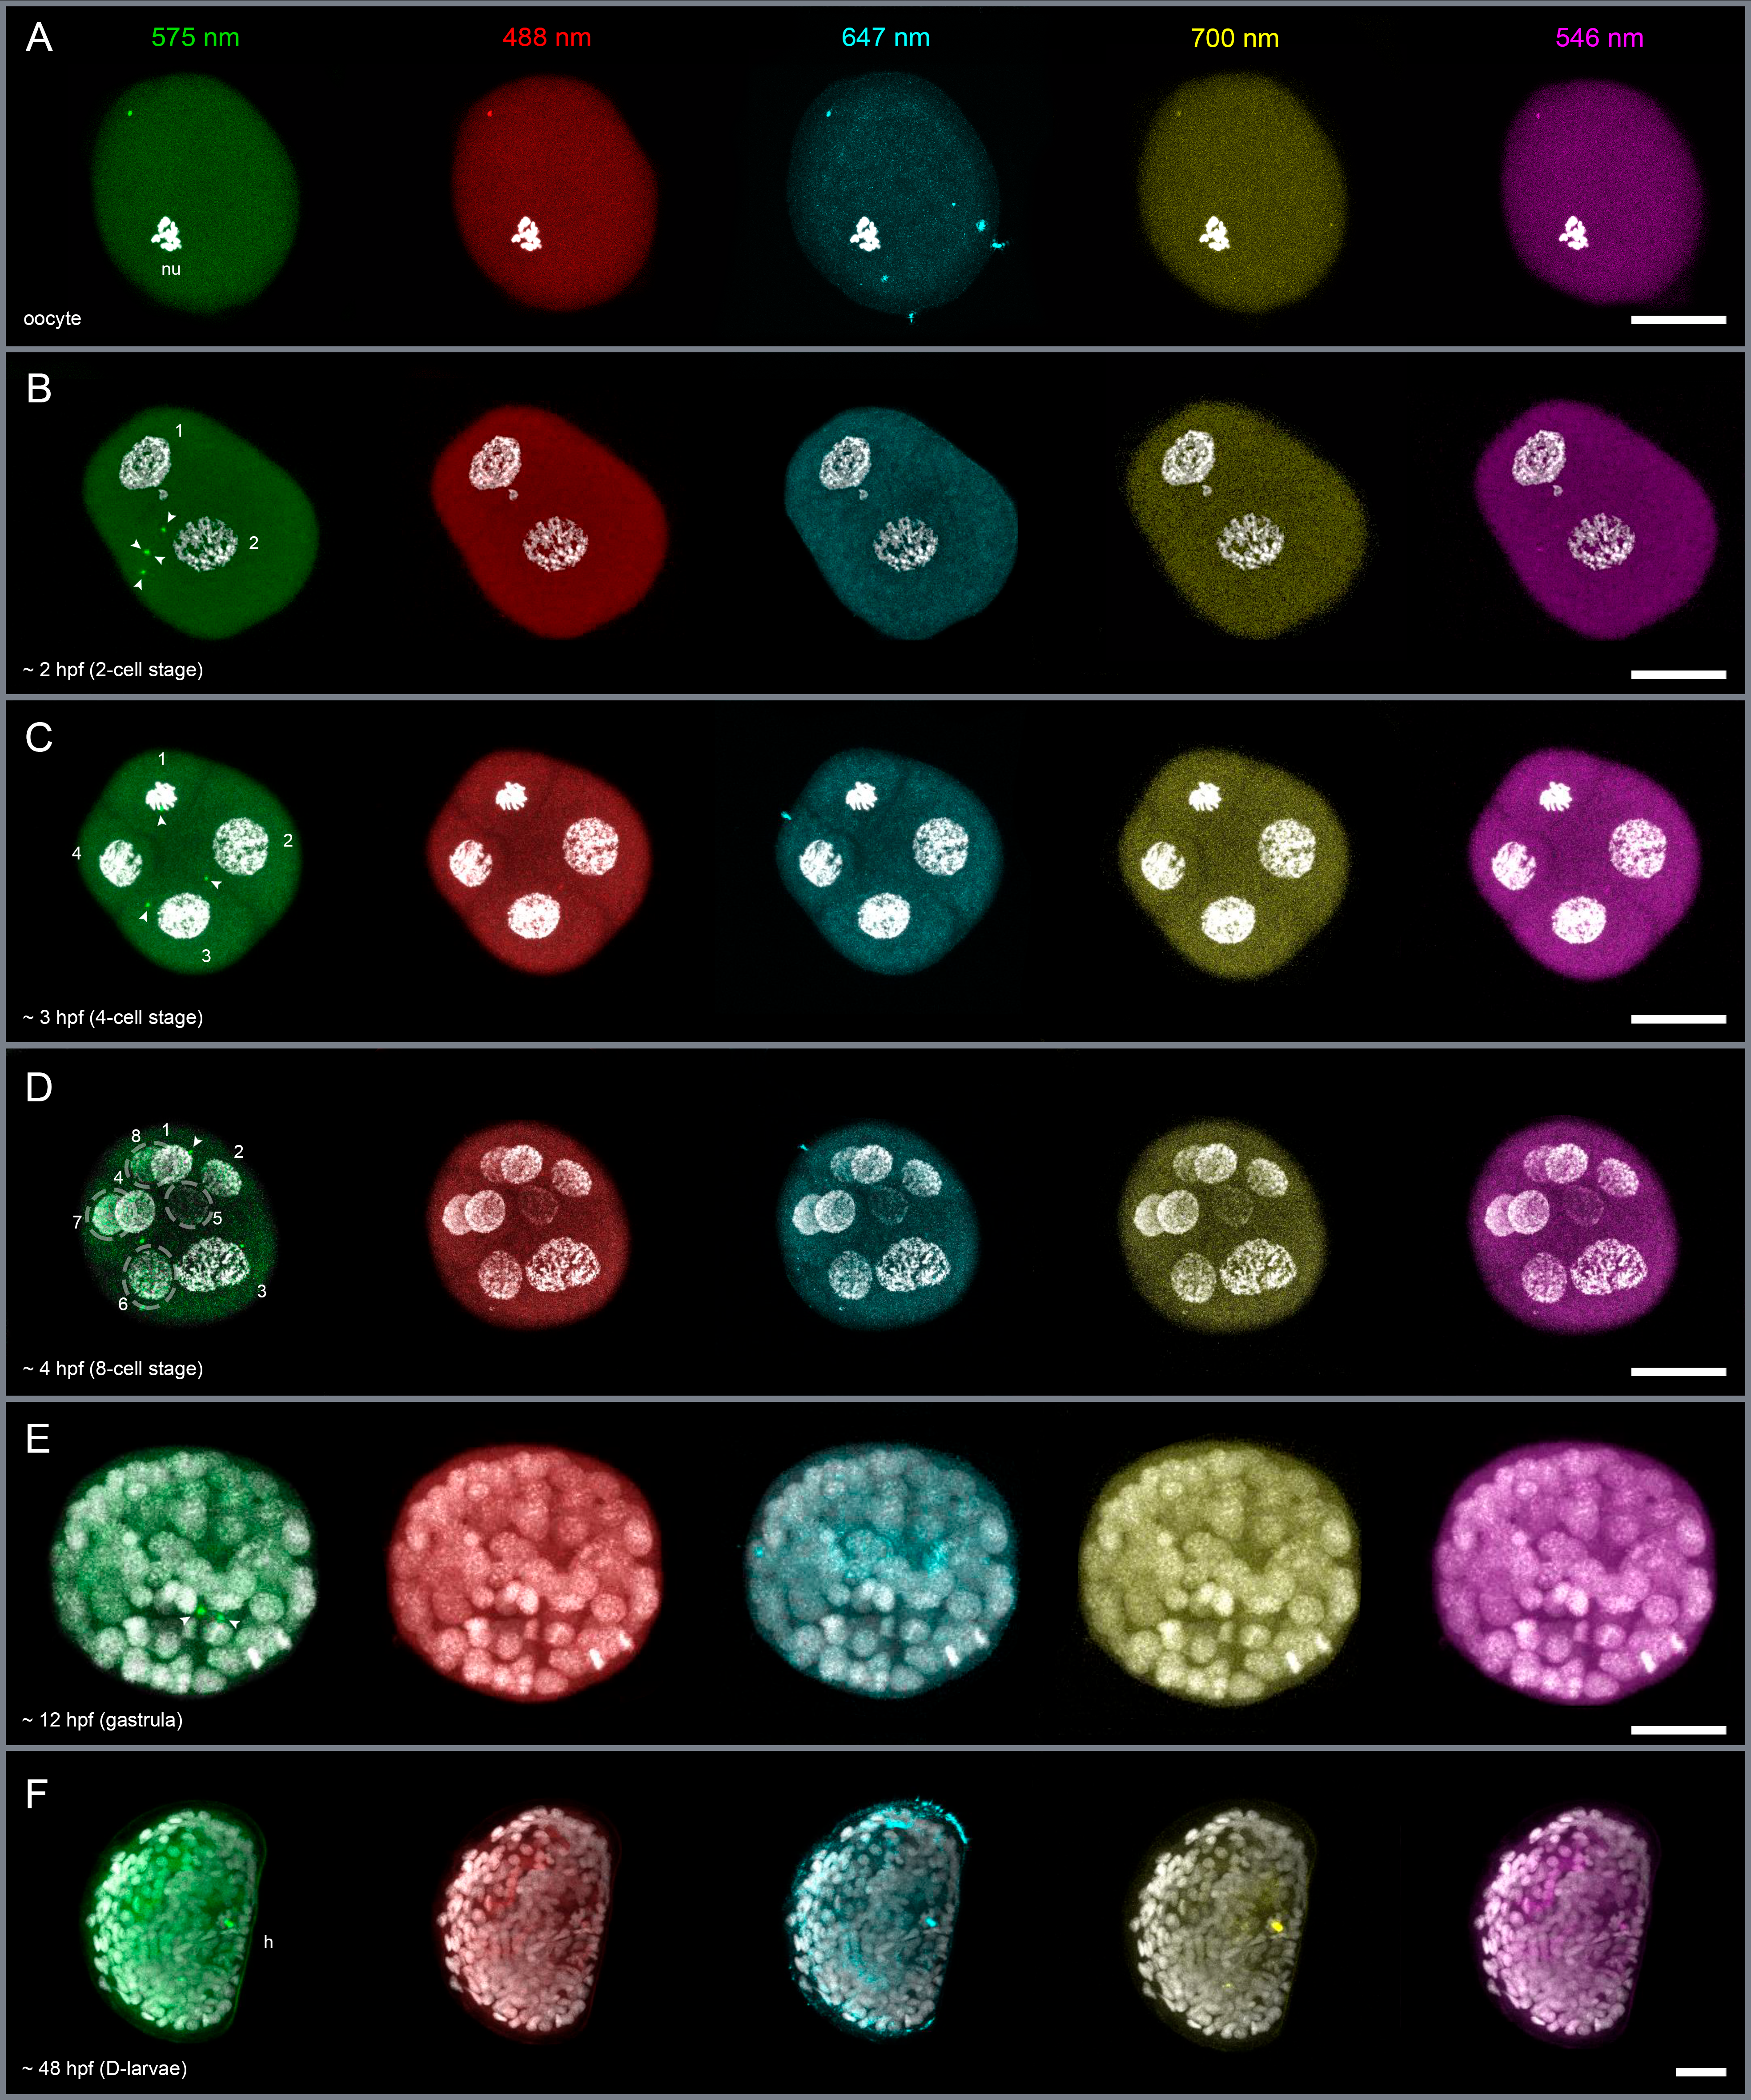
\includegraphics[width=0.9\textwidth]{supp_figures/supp_fig_S16.png}
	\caption[\textbf{MitoTracker staining and negative controls of mRNA \textit{in-situ} \gls{hcr} in in \gls{mgal} (A) oocyte, (B) 2-cell male embryo, (C) 4-cell female embryo, (D) 8-cell female embryo, (E) \qty{12}{\hpf} embryo (gastrula), and (F) \qty{48}{\hpf} larvae (D-veliger)}]
	{
		\textbf{MitoTracker staining and negative controls of mRNA \textit{in-situ} \gls{hcr} in \gls{mgal} (A) oocyte, (B) 2-cell male embryo, (C) 4-cell female embryo, (D) 8-cell female embryo, (E) \qty{12}{\hpf} embryo (gastrula), and (F) \qty{48}{\hpf} larvae (D-veliger)}. Nuclei are shown in white; in the 2-, 4-, and 8-cell stages, nuclei are also marked with numbers; in the 8-cell stage, nuclei of blastomeres in the background are highlighted with dashed circles. Sperm mitochondria, when stained (shown in green), are marked with arrowheads. Acquisition channels are indicated on top, and colours are the same as in \cref{fig:hcr}. h: hinge; nu: oocyte nucleus. Scale bar: \qty{20}{\um}.
	}
	\label{suppFig:hcrBianco}
\end{figure}

\afterpage{\clearpage
	\begin{figure}[ht!]
		\floatbox[{\capbeside\thisfloatsetup{capbesideposition={right,top},capbesidewidth=0.4\textwidth}}]{figure}[\FBwidth]
		{\includegraphics[width=0.5\textwidth]{supp_figures/supp_fig_S17.png}}
		{\caption[\textbf{MitoTracker staining and negative controls of Vasa immunolocalization in \gls{mgal} embryos}]
			{
				\textbf{MitoTracker staining and negative controls of Vasa immunolocalization in \gls{mgal} embryos}. Nuclei are shown in white. Sperm mitochondria (in green) are marked with arrowheads. pb: polar body. Scale bar: \qty{20}{\um}.
			}
			\label{suppFig:immunoBianco}}
	\end{figure}}

\clearpage

% \end{document}
\include{sections/supp_tables}
% \documentclass[../main.tex]{subfiles}

% \begin{document}

{
\setstretch{1.0}
\chapter*{Data availability}
\addcontentsline{toc}{chapter}{Data availability}
\label{data_availability}
\markboth{Data availability}{Data availability}
}

\normalsize
All the supplementary materials, as well as high-resolution figures and a parsabel versione of tables, are accessible online at the following GitHub repository:

\underline{\href{https://github.com/filonico/phd_thesis_tex}{https://github.com/filonico/phd\_thesis\_tex}}

% \end{document}

\newpage 
\ % empty page
\newpage

% activity report
{
\chapter*{Activity report}
\label{activityreport}
% \addcontentsline{toc}{chapter}{Activity report}
\markboth{Activity report}{Activity report}
}

\setcounter{page}{1}

\normalsize
\textit{This is the report of the activities carried out during my 3-year PhD course (2021--2024)}.

\section*{Research activity}
%\normalsize
\textit{Here are the research activities not directly related to the main topic of the PhD thesis.}
\begin{itemize}
    \item Manual curation of long interspersed nuclear element (LINE) libraries of several bivalve species;
    \item comparative genomics analysis of Hox and ParaHox genes in branchiopod crustaceans;
    \item comparative genomics analysis of branchiopod crustaceans to investigate the molecular underpinnnings of morphological stasis and genome size variations;
    \item molecular phylogenetics and Bayesian dating of branchiopod crustaceans;
    \item preparation of mRNA sequences of genes involved in body segmentation in \textit{Triops cancriformis} (Pancrustacea, Branchiopoda), to be used to generate probes for mRNA \textit{in-situ} HCR on larvae (in collaboration with the Patel Lab; Marine Biology Lab, Woods Hole, MA, USA);
    \item collection, fixation, and storing of jouvenile stages of several stick insect (Insecta, Phasmida) species, to be used for mRNA \textit{in-situ} HCR to investigate the temporal and spatial transcription of genes involved in wing morphogenesis (in collaboration with the Patel Lab; Marine Biology Lab, Woods Hole, MA, USA);
    \item preparation of a review on the evolutionary causes and consequences of trait loss reversals;
    \item preparation of mitotic chromosome plates in the red wood ant \textit{Formica paralugubris} from cerebral ganglia of pre-pupae.

\end{itemize}

\section*{Visiting scholar}
\begin{itemize}
    \item Nuzhdin Lab (University of Southern California, Los Angeles, CA, UA; \DTMDate{2023-08-20}--\DTMDate{2024-02-20}), to accomplish the abroad period of my PhD;
    \item Juan Pasantes\curlyapostrophe{} lab (University of Vigo, Vigo, Spain; \DTMshortmonthname{1} \ordinalnum{12}--\ordinalnum{22}, 2023), for a specific training on chromosome mitotic plate preparation in bivalve species.
\end{itemize}

\section*{Teaching activity}
\begin{itemize}
    \item Practical class \doublecurlyquotes{CAFE: estimating gene family turnover across a phylogenetic tree} (Apr 23, 2024) for first-year students of the course \doublecurlyquotes{Molecular phylogenetics} pursuing a Master degree in \doublecurlyquotes{Bioinformatics} at the University of Bologna (Italy);
    \item Practical invertebrate zoology class (\cvdateformatwithoutday{2022}{9}--\cvdateformatwithoutday{2023}{1}) for first-year students pursuing a Bachelor degree in \doublecurlyquotes{Biological Sciences} at the University of Bologna (Italy).
\end{itemize}

\section*{Co-supervised thesis}
\begin{itemize}
    \item \textit{Evaluation of different calibration methods on Branchiopoda (Crustacea) phylogeny}. Niccolò Righetti. Master degree in \doublecurlyquotes{Biodiversità ed evoluzione}, University of Bologna, Bologna (Italy). Supervisor: Andrea Luchetti. Co-supervisor: \underline{Filippo Nicolini}. AA 2022--2023;
    \item \textit{Filogenesi molecolare di alcune famiglie dell\curlyapostrophe ordine Phasmatodea con enfasi sulla famiglia Heteropterygidae (Bacilloidea)}. Giacomo Orsini. Bachelor degree in \doublecurlyquotes{Scienze biologiche}, University of Bologna, Bologna (Italy). Supervisor: Andrea Luchetti. Co-supervisor: Simona Corneti, \underline{Filippo Nicolini}. AA 2021--2022;
    \item \textit{Filogenesi molecolare di specie appartenenti alle famiglie Heteropterygidae e Anisacanthidae (Phasmatodea, Bacilloidea)}. Alessandro Siragusa Camacho. Bachelor degree in \doublecurlyquotes{Scienze biologiche}, University of Bologna, Bologna (Italy). Supervisor: Andrea Luchetti. Co-supervisor: Simona Corneti, \underline{Filippo Nicolini}. AA 2021/2022;
    \item \textit{Filogenesi molecolare di specie della famiglia Pseudophasmatidae}. Giovanni Amedeo Paselli. Bachelor degree in \doublecurlyquotes{Scienze biologiche}, University of Bologna, Bologna (Italy). Supervisor: Barbara Mantovani. Co-supervisors: Simona Corneti, \underline{Filippo Nicolini}. AA 2020--2021.
\end{itemize}

\section*{Courses and workshops}
\begin{itemize}
    \item \textit{Establishing state-of-the-art mollusc genomics}. EMBO Workshop. Namur, Belgium. \DTMshortmonthname{5} \ordinalnum{28}--\ordinalnum{31}, 2024;
    \item \textit{Art (Science) Attack}. Physalia Courses. Online. \DTMshortmonthname{5} \ordinalnum{20}--\ordinalnum{23}, 2024;
    \item \textit{Introduction to Python for biologists}. Physalia Courses. Online. \DTMshortmonthname{9} \ordinalnum25--\ordinalnum28, 2023;
    \item \textit{ITA*PHY phylogenetics workshop}. Trento, Italy. \DTMshortmonthname{1} \ordinalnum{6}--\ordinalnum{9}, 2023;
    \item \textit{Sex chromosome evolution}. Physalia Courses. Online. \DTMshortmonthname{1} \ordinalnum{23}--\ordinalnum{27}, 2023.
\end{itemize}

\section*{Awards and scholarships}
\begin{itemize}
    \item Travel grant to attend the \doublecurlyquotes{Evoluzione2024} congress in Naples (Italy). Stazione Zoologica Anton Dohrn. \DTMshortmonthname{9} \ordinalnum{8}--\ordinalnum{11}, 2024;
    \item Travel grant to attend the EMBO workshop \textit{Establishing state-of-the-art mollusc genomics} in Namur (Belgium). EMBO. \DTMshortmonthname{5} \ordinalnum{28}--\ordinalnum{31}, 2024;
    \item Laura Bassi scholarship for editorial assistance to postgraduates and junior academics. Editing Press. \DTMdate{2023-4-13}.
\end{itemize}

\section*{Presentations at congresses}
\subsection*{Oral presentations}
\begin{itemize}
    \item \underline{Nicolini F}, Iannello M, Piccinini G, Ghiselli F, Luchetti A, Milani L. (2024). Advancing the study of bivalve sex determination in the light of comparative genomics. Establishing state-of-the-art mollusc genomics (EMBO workshop). Namur (Belgium). May 27-30, 2024;
    \item \underline{Nicolini F}, Ghiselli F, Milani L, Luchetti A. (2023). Contrasting patterns of amino acid evolution and shared ancestry between putative sex-determining genes in bivalve molluscs. EVOLMAR 2023. Online. Nov 14-17, 2023;
    \item \underline{Nicolini F}, Ghiselli F, Milani L, Luchetti A. (2023). Sex-determination related genes in bivalves: novel acquisitions and high rates of sequence evolution. Evolution 2023 (Ernst Mayr Award symposium). Online. Jun 2-3, 2023.
\end{itemize}

\subsection*{Poster presentations}
\begin{itemize}
    \item \underline{Nicolini F}, Iannello M, Piccinini G, ghiselli F, Nuzhdin S, Luchetti A, Milani L. (2024). How to detect sex-determinig genes through molecular evolution: bivalves a a case study. Evoluzione 2024. Naples, Italy. Sep 8--11, 2024;
    \item \underline{Nicolini F}, Ghiselli F, Milani L, Luchetti A. (2022). Clues of accelerated molecular evolution in gene families associated wit sex determination in bivalves. SMBE 2023. Ferrara, Italy. Jul 24--27, 2023;
    \item \underline{Nicolini F}, Ghiselli F, Milani L, Luchetti A. (2022). Clues of accelerated molecular evolution in gene families associated wit sex determination in bivalves. SIBE/ISEB 2022. Ancona, Italy. Sep 4--7, 2022;
    \item \underline{Nicolini F}, Martelossi J, Forni G, Mantovani B, Luchetti A. (2021) First insights and comparative genomics of Hox and ParaHox genes in tadpole shrimps. EuroEvoDevo 2022. Naples, Italy. May 31--Jun 3, 2022.
\end{itemize}

\subsection*{Invited talks}
\begin{itemize}
    \item \textit{From comparative genomics to fluorescence imaging: a multi-disciplinary approach to study bivalve sex determination}. Auer Lab. University of Fribourg, Fribourg. Jul 26, 2024.
\end{itemize}

\subsection*{Outreach activity}
\begin{itemize}
    \item Editor and web writer for BioPills -- the Italian community of life sciences (\ulhref{https://biopills.net/}{biopills.net/}). Jul 2017--ongoing;
    \item Presenter at the European Researchers\curlyapostrophe{} Night 2024, University of Bologna, Bologna (Italy). Sep 27, 2024;
    \item Presenter at the BiGeA Day 2023, University of Bologna, Bologna (Italy). May 27, 2023;
    \item Opening Days, University of Bologna, Bologna (Italy). Nov 18, 2022.
\end{itemize}

\subsection*{Scientific publications}
\small{\textit{* equal contribution}}
\begin{itemize}
    \item Righetti N*, \underline{Nicolini F*}, Forni G, \& Luchetti A. (2024). Towards a time-tree solution for Branchiopoda diversification: a jackknife assessment of fossil age priors. \textit{Submitted for peer-review}
    \item \underline{Nicolini F}, Ghiselli F, Luchetti A, \& Milani L. (2023). Bivalves as emerging model systems to study the mechanisms and evolution of sex determination: a genomic point of view. \textit{Genome Biology and Evolution}, \textit{15}(10), evad181. doi: \ulhref{https://doi.org/10.1093/gbe/evad181}{10.1093/gbe/evad181}
    \item Martelossi J, \underline{Nicolini F}, Subacchi S, Pasquale D, Ghiselli F, \& Luchetti A. (2023). Multiple and diversified transposon lineages contribute to early and recent bivalve genome evolution. \textit{BMC Biology}, \textit{21}(1), 1--23. doi: \ulhref{https://doi.org/10.1186/s12915-023-01632-z}{10.1186/s12915-023-01632-z}
    \item \underline{Nicolini F}, Martelossi J, Forni G, Savojardo C, Mantovani B, \& Luchetti A. (2023). Comparative genomics of Hox and ParaHox genes among major lineages of Branchiopoda with emphasis on tadpole shrimps. \textit{Frontiers in Ecology and Evolution}, \textit{11}, 23. doi: \ulhref{https://doi.org/10.3389/fevo.2023.1046960}{10.3389/fevo.2023.1046960}
    \item Forni G, Cussigh A, Brock PD, Jones BR, \underline{Nicolini F}, Martelossi J, Luchetti A, \& Mantovani B. (2023). Taxonomic revision of the Australian stick insect genus \textit{Candovia} (Phasmida: Necrosciinae): insight from molecular systematics and species-delimitation approaches. \textit{Zoological Journal of the Linnean Society}, \textit{197}(1), 189--210. doi: \ulhref{https://doi.org/10.1093/zoolinnean/zlac074}{10.1093/zoolinnean/zlac074}
\end{itemize}

\end{document}
